%definira klasu dokumenta 
\documentclass[12pt]{report} 

%prostor izmedu naredbi \documentclass i \begin{document} se zove uvod. U njemu se nalaze naredbe koje se odnose na cijeli dokument

%osnovni LaTex ne može riješiti sve probleme, pa se koriste različiti paketi koji olakšavaju izradu željenog dokumenta
\usepackage[croatian]{babel} 
\usepackage{amssymb}
\usepackage{amsmath}
\usepackage{txfonts}
\usepackage{mathdots}
\usepackage{titlesec}
\usepackage{array}
\usepackage{lastpage}
\usepackage{etoolbox}
\usepackage{tabularray}
\usepackage{color, colortbl}
\usepackage{adjustbox}
\usepackage{geometry}
\usepackage[classicReIm]{kpfonts}
\usepackage{hyperref}
\usepackage{fancyhdr}

\usepackage{float}
\usepackage{setspace}
\restylefloat{table}


\patchcmd{\chapter}{\thispagestyle{plain}}{\thispagestyle{fancy}}{}{} %redefiniranje stila stranice u paketu fancyhdr

%oblik naslova poglavlja
\titleformat{\chapter}{\normalfont\huge\bfseries}{\thechapter.}{20pt}{\Huge}
\titlespacing{\chapter}{0pt}{0pt}{40pt}


\linespread{1.3} %razmak između redaka

\geometry{a4paper, left=1in, top=1in,}  %oblik stranice

\hypersetup{ colorlinks, citecolor=black, filecolor=black, linkcolor=black,	urlcolor=black }   %izgled poveznice


%prored smanjen između redaka u nabrajanjima i popisima
\newenvironment{packed_enum}{
	\begin{enumerate}
		\setlength{\itemsep}{0pt}
		\setlength{\parskip}{0pt}
		\setlength{\parsep}{0pt}
	}{\end{enumerate}}

\newenvironment{packed_item}{
	\begin{itemize}
		\setlength{\itemsep}{0pt}
		\setlength{\parskip}{0pt}
		\setlength{\parsep}{0pt}
	}{\end{itemize}}




%boja za privatni i udaljeni kljuc u tablicama
\definecolor{LightBlue}{rgb}{0.9,0.9,1}
\definecolor{LightGreen}{rgb}{0.9,1,0.9}

%Promjena teksta za dugačke tablice
\DefTblrTemplate{contfoot-text}{normal}{Nastavljeno na idućoj stranici}
\SetTblrTemplate{contfoot-text}{normal}
\DefTblrTemplate{conthead-text}{normal}{(Nastavljeno)}
\SetTblrTemplate{conthead-text}{normal}
\DefTblrTemplate{middlehead,lasthead}{normal}{Nastavljeno od prethodne stranice}
\SetTblrTemplate{middlehead,lasthead}{normal}

%podesavanje zaglavlja i podnožja

\pagestyle{fancy}
\lhead{Programsko inženjerstvo}
\rhead{$<$Projektni zadatak$>$}
\lfoot{$<$Naziv grupe$>$}
\cfoot{stranica \thepage/\pageref{LastPage}}
\rfoot{\today}
\renewcommand{\headrulewidth}{0.2pt}
\renewcommand{\footrulewidth}{0.2pt}


\begin{document} 
	
	
	
	\begin{titlepage}
		\begin{center}
			\vspace*{\stretch{1.0}} %u kombinaciji s ostalim \vspace naredbama definira razmak između redaka teksta
			\LARGE Programsko inženjerstvo\\
			\large Ak. god. 2020./2021.\\
			
			\vspace*{\stretch{3.0}}
			
			\huge Ozdravi – olakšava život kad imate bolesnu djecu\\
			\Large Dokumentacija, Rev. \textit{$<$1 ili 2$>$}\\
			
			\vspace*{\stretch{12.0}}
			\normalsize
			Grupa: \textit{Proggy i Žohari}\\
			Voditelj: \textit{Jan Komerički}\\
			
			
			\vspace*{\stretch{1.0}}
			Datum predaje: \textit{$<$dan$>$. $<$mjesec$>$. $<$godina$>$.}\\
	
			\vspace*{\stretch{4.0}}
			
			Nastavnik: \textit{$<$Ime i prezime nastavnika zaduženog za vašu grupu$>$}\\
		
		\end{center}

	
	\end{titlepage}

	
	\tableofcontents


	\chapter{Dnevnik promjena dokumentacije}
				
		
		\begin{longtblr}[
				label=none
			]{
				width = \textwidth, 
				colspec={|X[2]|X[13]|X[3]|X[3]|}, 
				rowhead = 1
			}
			\hline
			\textbf{Rev.}	& \textbf{Opis promjene/dodatka} & \textbf{Autori} & \textbf{Datum}\\[3pt] \hline
			0.1 & Napravljen predložak.	& J.K. & 18.10.2023. 		\\[3pt] \hline 
			0.2.1	& Napisan dio opisa projektnog zadatka i funkcionalni zahtjevi & J.K. & 26.10.2023. 	\\[3pt] \hline 
			0.2.2   & Napisani \textit{use cases} za neregistriranog korisnika i roditelja. & J.K. & 28.10.2023. \\[3pt] \hline 
			0.2.3   & Završeni \textit{use cases} i završen Opis projektnog zadatka & J.K. & 2.11.2023. \\[3pt] \hline 
			0.3.1 & Napisan opis baze podataka, ispravljene greške u \textit{use cases}& J.K. & 11.11.2023. \\[3pt] \hline 
			0.3.2 & Napisan opis arhitekture sustava, uneseni dijagrami za istog i za bazu podataka, popravljene sitne pogreške & J.K.,K.Č., L.M. & 14.11.2023. \\[3pt] \hline 
			0.10 & Preveden uvod & * & 08.09.2013. \\[3pt] \hline 
			0.11 & Sekvencijski dijagrami & * & 09.09.2013. \\[3pt] \hline 
			0.12.1 & Započeo dijagrame razreda & * & 10.09.2013. \\[3pt] \hline 
			0.12.2 & Nastavak dijagrama razreda & * & 11.09.2013. \\[3pt] \hline 
			\textbf{1.0} & Verzija samo s bitnim dijelovima za 1. ciklus & * & 11.09.2013. \\[3pt] \hline 
			1.1 & Uređivanje teksta -- funkcionalni i nefunkcionalni zahtjevi & * \newline * & 14.09.2013. \\[3pt] \hline 
			1.2 & Manje izmjene:Timer - Brojilo vremena & * & 15.09.2013. \\[3pt] \hline 
			1.3 & Popravljeni dijagrami obrazaca uporabe & * & 15.09.2013. \\[3pt] \hline 
			1.5 & Generalna revizija strukture dokumenta & * & 19.09.2013. \\[3pt] \hline 
			1.5.1 & Manja revizija (dijagram razmještaja) & * & 20.09.2013. \\[3pt] \hline 
			\textbf{2.0} & Konačni tekst predloška dokumentacije  & * & 28.09.2013. \\[3pt] \hline 
			&  &  & \\[3pt] \hline	
		\end{longtblr}
	
	
		\textit{Moraju postojati glavne revizije dokumenata 1.0 i 2.0 na kraju prvog i drugog ciklusa. Između tih revizija mogu postojati manje revizije već prema tome kako se dokument bude nadopunjavao. Očekuje se da nakon svake značajnije promjene (dodatka, izmjene, uklanjanja dijelova teksta i popratnih grafičkih sadržaja) dokumenta se to zabilježi kao revizija. Npr., revizije unutar prvog ciklusa će imati oznake 0.1, 0.2, …, 0.9, 0.10, 0.11.. sve do konačne revizije prvog ciklusa 1.0. U drugom ciklusu se nastavlja s revizijama 1.1, 1.2, itd.}
	\chapter{Opis projektnog zadatka}
		
		\text Cilj ovog projekta razviti je programsku podršku za web aplikaciju \textit{Ozdravi} koja će korisnicima omogućiti olakšanu komunikaciju s pedijatrom i liječnikom obiteljske medicine, te lakši pregled podataka o pregledima sebe i svojeg djeteta. Uz to, aplikacija će automatizirati slanje preporuka za bolovanje i ispričnica, uvelike štedeći vrijeme roditeljima koji zbog toga neće morati naknadno ići po imenovane potvrde.\\
		Do sada, kada bi dijete obolilo, roditelji bi trebali gubiti mnogo vremena u komunikaciji s pedijatrom, te kontinuiranim preuzimanjem i prenošenjem raznih potvrda, bilo ispričnica ili preporuka i doznaka za bolovanje. Naum ove aplikacije jest automatizacija slanja tih potvrda, te olakšani pregled medicinskih podataka djece. \\
		
		\section{Korisnički zahtjevi}
		Korisnički zahtjevi su sljedeći:
		\begin{packed_item}
			
			\item  mogućnost samostalne registracije i prijave roditelja
			\item  roditeljski pristup profilima sebe i sve svoje djece, u kojima je omogućen pristup pripadnim medicinskim kartonima
			\item  primanje obavijesti od pedijatra vezano uz pojedino dijete
			\item  mogućnost učitavanja privatnih nalaza i primanja povratnih informacija od pedijatra
			\item  pedijatri/liječnici moraju imati mogućnost unosa novog pacijenta
			\item  pedijatri/liječnici obiteljske medicine imaju pristup popisu svih svojih pacijenata, njihovim informacijama i mogućnost upisivanja novog pregleda
			\item  pedijatri moraju imati mogućnost generiranja i automatskog slanja ispričnica i preporuka za bolovanje
			\item  pedijatri i liječnici moraju imati mogućnost pisanja uputnica za specijalističke preglede, te slanje potencijalnih lokacija za iste roditeljima
			\item  liječnici obiteljske medicine moraju imati mogućnost potvrđivanja preporuka za bolovanje i slanja doznaka o istom
			\item  administratori moraju imati mogućnost brisanja i uređivanja korisničkih računa, stvaranja računa liječnika i pedijatra, te stvaranja i povezivanja profila djece s roditeljem
			
		\end{packed_item}
		Analizom korisničkih zahtjeva, razvojni tim došao je do zaključka da je stvaranje profila djece od strane administratora nepraktično, te da postoji efikasnije rješenje. Ono je stvaranje profila djece od strane pedijatra pri prvome pregledu, s obzirom na to da pedijatri imaju pristup osobnim podacima djece. 
		
		\section{Opis korištenja aplikacije}
		
		Prilikom pokretanja aplikacije neprijavljenom korisniku prikazat će se naslovna web stranica s opisom funkcionalnosti aplikacije, katalogom usluga, te opcijama za registraciju ili prijavu. \\
		Prilikom registracije korisnik unosi sljedeće podatke:
		\begin{packed_item}
			
			\item  korisničko ime
			\item  email adresa
			\item  lozinka
			\item  ime
			\item  prezime
			\item  OIB
			\item  mjesto prebivališta
			\item  poštanski broj prebivališta
			\item  email adresa poslodavca
			\item  broj telefona
			
		\end{packed_item}
		Registracijom u sustav, korisnik dobiva prava roditelja. Naknadna promjena prava je nemoguća. Ostale uloge se ne registriraju, već su dodane u sustav od strane administratora. 
		
		\underbar{\textit{Roditelj}} prijavom u sustav koristeći svoje korisničko ime i lozinku dolazi do uvodne stranice za roditelje. Na uvodnoj stranici nalaze se obavijesti od liječnika obiteljske medicine i pedijatra, te izbornik mogućih profila kojima roditelj može pristupiti. Roditelj ima omogućen pristup svojem profilu i profilima svoje djece. Nakon biranja profila, otvara se nova stranica na kojoj se nalazi izbornik mogućnosti, te prostor za prikaz. \\
		Unutar profila djeteta, izbornik sadrži sljedeće opcije:
		\begin{packed_item}
			
			\item  Obavijesti - otvara prikaz svih obavijesti od pedijatra zaduženog za navedeno dijete
			\item  Povijest liječničkih pregleda - otvara svojevrstan medicinski karton djeteta
			\item  Generirane ispričnice - otvara pregled generiranih ispričnica koje pedijatar izdaje djetetu
			\item  Nalazi iz laboratorija - otvara pregled nalaza djeteta koji su naknadno dobiveni iz laboratorija
			\item  Specijalistički pregledi - otvara stranicu na kojoj pedijatar šalje potvrdu za specijalistički pregled i lokacije na kojima je moguće izvršiti navedeni pregled
			\item  Učitavanje nalaza - opcija koja omogućuje \textit{upload} nalaza koji je dobiven pri eventualnom pregledu kod privatnika
		
		\end{packed_item}
		Unutar profila roditelja, izbornik sadrži sljedeće opcije:
			\begin{packed_item}
			
			\item  Obavijesti - otvara prikaz svih obavijesti od liječnika zaduženog za roditelja
			\item  Povijest liječničkih pregleda - otvara svojevrstan medicinski karton roditelja
			\item  Potvrđena bolovanja - otvara pregled bolovanja koja su odobrena od strane liječnika
			\item  Specijalistički pregledi - otvara stranicu na kojoj liječnik šalje potvrdu za specijalistički pregled i lokacije na kojima je moguće izvršiti navedeni pregled
			\item  Učitavanje nalaza - opcija koja omogućuje \textit{upload} nalaza koji je dobiven pri eventualnom pregledu kod privatnika
			
		\end{packed_item}
		
		\noindent Osim roditelja, postoje još tri vrste korisnika:
		
		\begin{packed_item}
			
			\item  pedijatar
			\item  liječnik obiteljske medicine
			\item  administrator
			
		\end{packed_item}	
		
		\underbar{\textit{Pedijatar/liječnik obiteljske medicine}} prijavom u sustav, koristeći korisničko ime i lozinku, ulazi na stranicu na kojoj je otvoren popis pacijenata. Moguć je odabir pojedinog pacijenta, čime se otvara profil tog pacijenta. Na profilu su vidljivi osnovni osobni podaci, te nekoliko gumba s opcijama. Te opcije su:
		
		\begin{packed_item}
			
			\item  Medicinski karton - otvara medicinski karton odabranog pacijenta
			\item  Novi pregled - otvara sučelje za unos novog pregleda odabranog pacijenta
			\item  Generiranje ispričnice (opcija samo za pedijatra) - otvara sučelje za generiranje ispričnice za odabranog pacijenta
			\item  Generiranje preporuke za bolovanje  (opcija samo za pedijatra) - otvara sučelje za generiranje preporuke za bolovanje za roditelja odabranog pacijenta
			\item  Nalazi iz privatnih ustanova - otvara popis nalaza iz privatnih ustanova za odabranog pacijenta
			\item  Specijalistički pregled - otvara sučelje za naručivanje odabranog pacijenta na specijalistički pregled
			\item  Potvrda bolovanja (opcija samo za liječnika obiteljske medicine) - otvara sučelje za potvrdu preporuka za bolovanje/otvaranje bolovanja
			
		\end{packed_item}
		
		S iznad glavnog sučelja nalazi se izbornik sa dvije opcije:
		
		\begin{packed_item}
			
			\item  Popis pacijenata - otvara već spomenuti popis pacijenata
			\item  Novi pacijent - otvara sučelje za unos novog pacijenta prilikom prvog pregleda
			\item  Preporuke za bolovanje (opcija samo za LOM-a) - otvara sučelje za potvrđivanje preporuka za bolovanje koje dobije od pedijatra
			
		\end{packed_item}	
		
		\underbar{\textit{Administrator}} sustava posjeduje najveće ovlasti od svih vrsta korisnika. On ima pristup bazi s popisom svih korisnika. Administrator ima mogućnost te korisnike brisati i mijenjati im podatke i međusobne veze (npr. promijeniti zaduženog pedijatra djetetu). Uz to, administrator je zadužen za stvaranje korisničkih računa za pedijatre i liječnike obiteljske medicine.\\
		
		\section{Postojeća slična rješenja}
		Već postoji web-aplikacija koja vrši sličan posao kao ovaj projekt. Radi se o portalu na platformi \textit{e-Građani}, pod nazivom \textit{Portal zdravlja}. Ipak, to rješenje vrlo je općenito. Imenovana aplikacija ne specijalizira se za dječju medicinsku brigu, već je platforma gdje punoljetni građani imaju pristup raznim uslugama hrvatskog zdravstva. Na primjer, građani imaju mogućnost naručivanja na preglede i cijepljenje, pregleda svojih posjeta liječniku, te pristup popisu lijekova koji su im pripisani, te još mnoge mogućnosti. Jedna sličnost koju valja primijetiti jest sekcija za specijalističke preglede. Ipak, na \textit{Portalu zdravlja} može se pristupiti samo prijašnjim nalazima, i ne nudi se mogućnost prikaza lokacija za pregled na karti.
		\begin{figure}[H]
			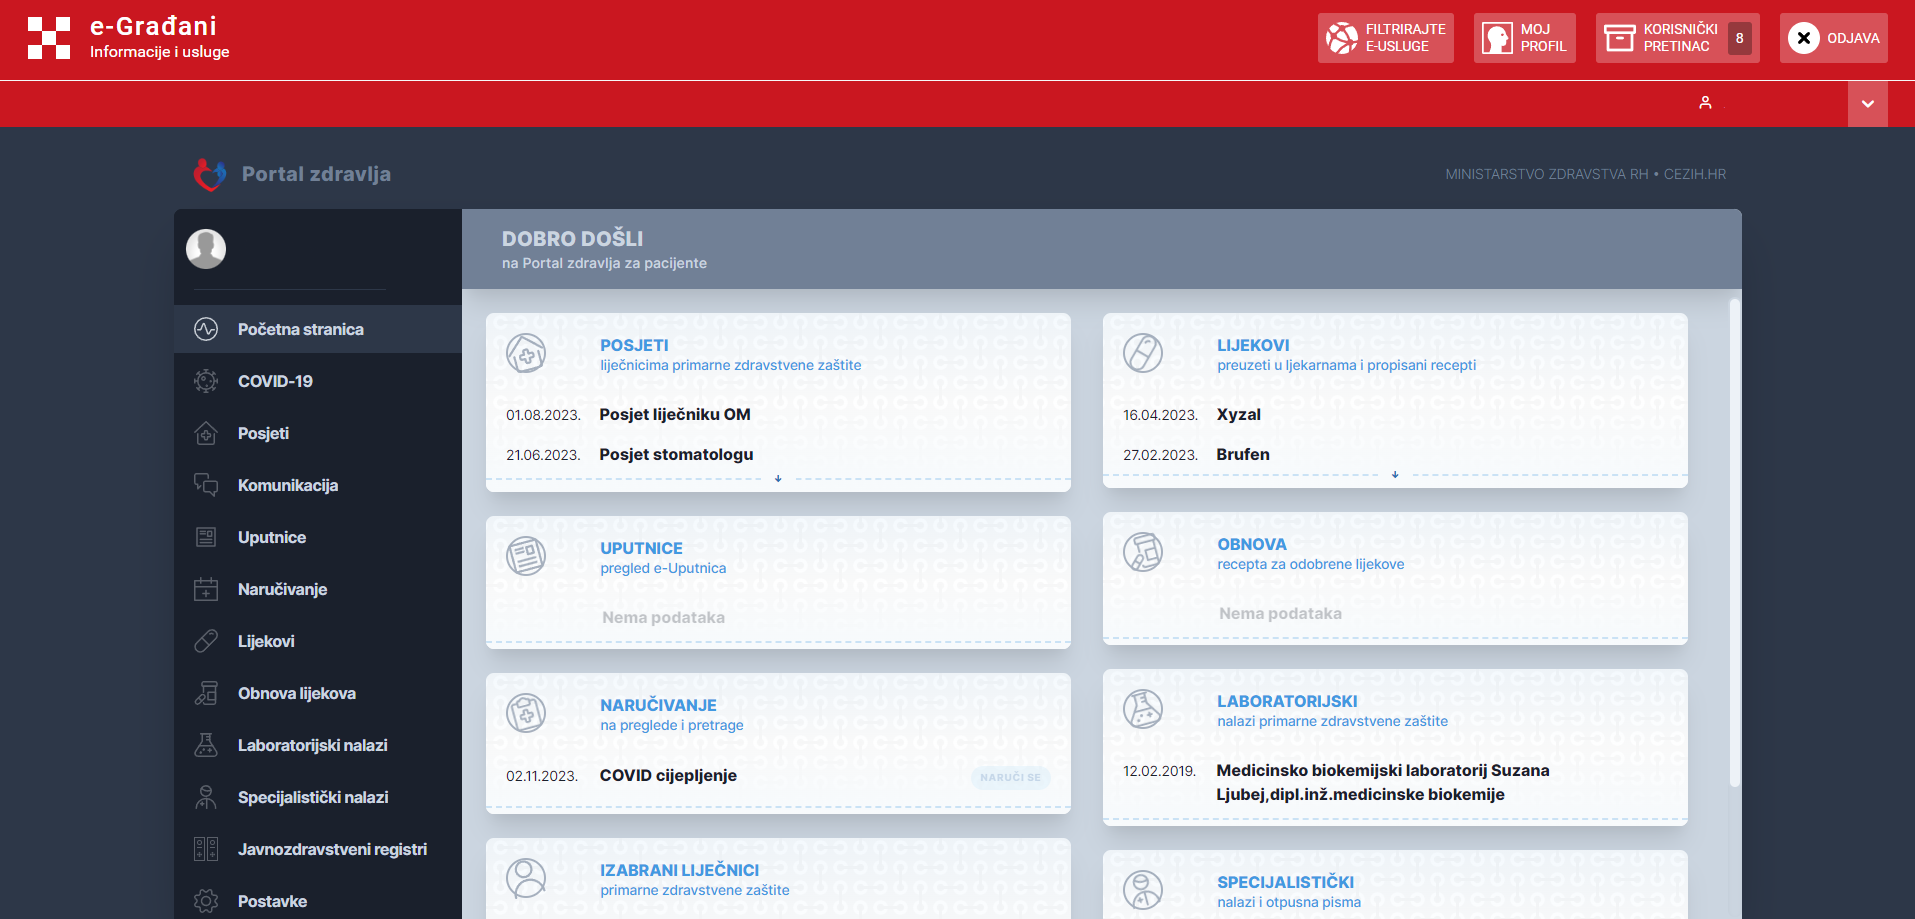
\includegraphics[scale=0.4]{slike/portalzdravlje.PNG} %veličina slike u odnosu na originalnu datoteku i pozicija slike
			\centering
			\caption{Izgled početnog izbornika platforme \textit{Portal zdravlja}}
			\label{fig:portal-zdravlja}
		\end{figure}
		
		\section{Opseg i prilagodljivost projektnog zadatka}
		Opisan rad aplikacije ostvaren je korištenjem nekoliko alata. Najprije, za razvoj \textit{backend-a} koristili smo alat \textit{Spring Boot}, gdje smo programirali u programskom jeziku Java. Za bazu podataka koristili smo \textit{H2} koji je također prilagođen radu u Javi, a za razvoj \textit{frontend-a} koristili smo \textit{React}, biblioteku programskog jezika JavaScript. \\
		Aplikacija (prilagodljivost-dodati).
		
		
		\section{Primjeri u \LaTeX u}
		
		\textit{Ovo potpoglavlje izbrisati.}\\

		U nastavku se nalaze različiti primjeri kako koristiti osnovne funkcionalnosti \LaTeX a koje su potrebne za izradu dokumentacije. Za dodatnu pomoć obratiti se asistentu na projektu ili potražiti upute na sljedećim web sjedištima:
		\begin{itemize}
			\item Upute za izradu diplomskog rada u \LaTeX u - \url{https://www.fer.unizg.hr/_download/repository/LaTeX-upute.pdf}
			\item \LaTeX\ projekt - \url{https://www.latex-project.org/help/}
			\item StackExchange za Tex - \url{https://tex.stackexchange.com/}\\
		
		\end{itemize} 	


		
		\noindent \underbar{podcrtani tekst}, \textbf{podebljani tekst}, 	\textit{nagnuti tekst}\\
		\noindent \normalsize primjer \large primjer \Large primjer \LARGE {primjer} \huge {primjer} \Huge primjer \normalsize
				
		\begin{packed_item}
			
			\item  primjer
			\item  primjer
			\item  primjer
			\item[] \begin{packed_enum}
				\item primjer
				\item[] \begin{packed_enum}
					\item[1.a] primjer
					\item[b] primjer
				\end{packed_enum}
				\item primjer
			\end{packed_enum}
			
		\end{packed_item}
		
		\noindent primjer url-a: \url{https://www.fer.unizg.hr/predmet/proinz/projekt}
		
		\noindent posebni znakovi: \# \$ \% \& \{ \} \_ 
		$|$ $<$ $>$ 
		\^{} 
		\~{} 
		$\backslash$ 
		
		
		\begin{longtblr}[
			label=none,
			entry=none
			]{
				width = \textwidth,
				colspec={|X[8,l]|X[8, l]|X[16, l]|}, 
				rowhead = 1,
			} %definicija širine tablice, širine stupaca, poravnanje i broja redaka naslova tablice
			\hline \SetCell[c=3]{c}{\textbf{naslov unutar tablice}}	 \\ \hline[3pt]
			\SetCell{LightGreen}IDKorisnik & INT	&  	Lorem ipsum dolor sit amet, consectetur adipiscing elit, sed do eiusmod  	\\ \hline
			korisnickoIme	& VARCHAR &   	\\ \hline 
			email & VARCHAR &   \\ \hline 
			ime & VARCHAR	&  		\\ \hline 
			\SetCell{LightBlue} primjer	& VARCHAR &   	\\ \hline 
		\end{longtblr}
		

		\begin{longtblr}[
				caption = {Naslov s referencom izvan tablice},
				entry = {Short Caption},
			]{
				width = \textwidth, 
				colspec = {|X[8,l]|X[8,l]|X[16,l]|}, 
				rowhead = 1,
			}
			\hline
			\SetCell{LightGreen}IDKorisnik & INT	&  	Lorem ipsum dolor sit amet, consectetur adipiscing elit, sed do eiusmod  	\\ \hline
			korisnickoIme	& VARCHAR &   	\\ \hline 
			email & VARCHAR &   \\ \hline 
			ime & VARCHAR	&  		\\ \hline 
			\SetCell{LightBlue} primjer	& VARCHAR &   	\\ \hline 
		\end{longtblr}
	


		
		
		%unos slike
		\begin{figure}[H]
			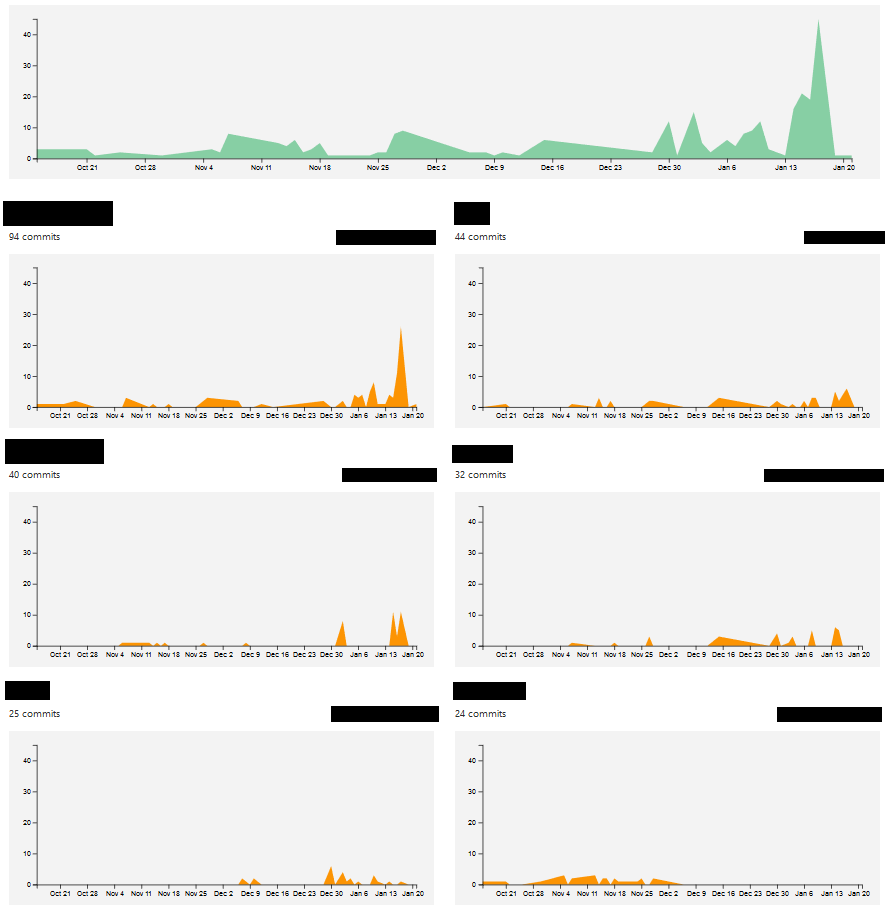
\includegraphics[scale=0.4]{slike/aktivnost.PNG} %veličina slike u odnosu na originalnu datoteku i pozicija slike
			\centering
			\caption{Izgled početnog izbornika platforme \textit{Portal zdravlja}}
			\label{fig:portal-zdravlja}
		\end{figure}
		
		\begin{figure}[H]
			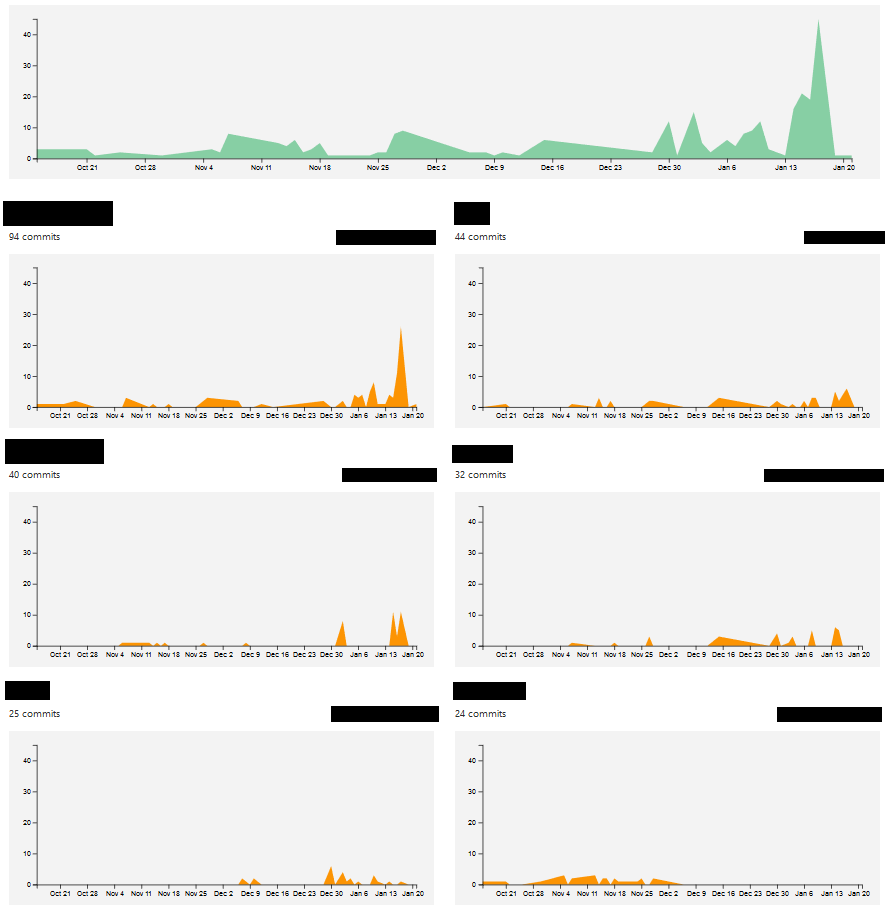
\includegraphics[width=\textwidth]{slike/aktivnost.PNG} %veličina u odnosu na širinu linije
			\caption{Primjer slike s potpisom 2}
			\label{fig:promjene2} %label mora biti drugaciji za svaku sliku
		\end{figure}
		
		Referenciranje slike \ref{fig:promjene2} u tekstu.
		
		\eject
		
	
	\chapter{Specifikacija programske potpore}
		
	\section{Funkcionalni zahtjevi}
			\noindent \textbf{Dionici:}
			
			\begin{packed_enum}
				
				\item Vlasnik (naručitelj)
				\item Neregistrirani korisnik
				\item Roditelji				
				\item Liječnici i pedijatri
				\item Administrator
				\item Razvojni tim
				
			\end{packed_enum}
			
			\noindent \textbf{Aktori i njihovi funkcionalni zahtjevi:}
			
			
			\begin{packed_enum}
				\item  \underbar{Neregistrirani/neprijavljeni korisnik (inicijator) može:}
				
				\begin{packed_enum}
					
					\item pregledati katalog usluga aplikacije
					\item vidjeti koje sve vrste korisnika aplikacija podržava
					\item registrirati se u sustav, koristeći korisničko ime, email adresu, lozinku, ime, prezime i OIB, čime stvara osobni korisnički račun
					\item prijaviti se u sustav putem korisničkog imena i lozinke
					
				\end{packed_enum}
			
				\item  \underbar{Roditelj (inicijator) može:}
				
				\begin{packed_enum}
					
					\item pristupiti profilima svoje djece ili svojem profilu
					\item otvarati i čitati obavijesti vezane uz svaki profil, poslane od liječnika ili pedijatra
					\item vidjeti svoj ili djetetov medicinski karton te povijest pregleda
					\item pristupiti ispričnicama generiranim za pojedino dijete te potvrdama o bolovanju
					\item pristupiti naknadnim nalazima laboratorijskih pretraga
					\item primiti informacije i narudžbe na specijalističke preglede, te vidjeti lokacije na kojima je moguće izvesti navedeni pregled
					\item učitati (\textit{uploadati}) nalaze koje dobije prilikom pregleda u privatnoj ordinaciji
					
				\end{packed_enum}
				
				\item  \underbar{Pedijatar (inicijator) može:}
				
				\begin{packed_enum}
					
					\item pristupiti profilima djece kojima je dedicirani pedijatar
					\item pristupiti liječničkim kartonima svih svojih pacijenata
					\item prijaviti novo dijete prilikom prvog pregleda, koristeći osobne podatke djeteta (ime, prezime, OIB, datum rođenja), te OIB roditelja
					\item za svakog pacijenta unijeti novi pregled
					\item za svakog pacijenta generirati ispričnicu
					\item za roditelje djece preporučiti bolovanje
					\item naručiti dijete na specijalistički pregled, te preporučiti lokacije za izvedbu istog
					
				\end{packed_enum}
				
				\item  \underbar{Liječnik obiteljske medicine(inicijator) može:}
				
				\begin{packed_enum}
					
					\item pristupiti profilima roditelja kojima je liječnik
					\item pristupiti liječničkim kartonima svih svojih pacijenata
					\item za svakog pacijenta unijeti novi pregled
					\item potvrditi ili odbiti preporuke za bolovanje roditelja
					\item naručiti roditelja na specijalistički pregled, te preporučiti lokacije za izvedbu istog
					
				\end{packed_enum}
				
				\item  \underbar{Administrator(inicijator) može:}
				
				\begin{packed_enum}
					
					\item vidjeti popis svih registriranih korisnika i njihovih osobnih podataka
					\item brisati korisnike
					\item mijenjati veze između korisnika, npr. premjestiti dijete s profila jednog roditelja na profil drugog
					\item stvarati profile liječnika i pedijatara
					
				\end{packed_enum}
				
				\item  \underbar{Baza podataka(sudionik):}
				
				\begin{packed_enum}
					
					\item pohranjuje sve podatke o korisnicima, njihove međusobne povezanosti i uloge
					\item pohranjuje liječničke kartone i dijagnoze roditelja i djece
					
				\end{packed_enum}
				
			\end{packed_enum}
			
			\eject 
			
			
				
			\subsection{Obrasci uporabe}
					\noindent \underbar{\textbf{UC1 - Pregledaj usluge aplikacije}}
					\begin{packed_item}
	
						\item \textbf{Glavni sudionik: }Neprijavljeni korisnik
						\item  \textbf{Cilj:} Upoznati se s mogućnostima aplikacije
						\item  \textbf{Sudionici:}-
						\item  \textbf{Preduvjet:}-
						\item  \textbf{Opis osnovnog tijeka:}
						
						\item[] \begin{packed_enum}
	
							\item Korisnik otvara web stranicu aplikacije
							\item Korisnik pregledava sadržaj stranice
						\end{packed_enum}
						\item  \textbf{Opis mogućih odstupanja:}
						\item[] \begin{packed_item}
						
							\item[1.a] Neuspjeh učitavanja stranice, zbog greške u pristupu serverima
							\item[] \begin{packed_enum}
							
								\item Korisnika se obavještava o neuspjehu učitavanja stranice putem ispisane poruke
								\item Korisnik provjerava svoj pristup internetu, te pokušava ponovno
							
							\end{packed_enum}
						\end{packed_item}
					\end{packed_item}
					\noindent \underbar{\textbf{UC2-Registriraj se}}
					\begin{packed_item}
						
						\item \textbf{Glavni sudionik: }Neregistrirani korisnik
						\item  \textbf{Cilj:} Stvoriti korisnički račun roditelja za prijavu u sustav
						\item  \textbf{Sudionici:} Baza podataka
						\item  \textbf{Preduvjet:} Otvorena početna stranica aplikacije
						\item  \textbf{Opis osnovnog tijeka:}
						
						\item[] \begin{packed_enum}
							
							\item Na početnoj stranici aplikacije korisnik odabire opciju "Registriraj se"
							\item Sustav otvara ekran registracije
							\item Korisnik unosi osobne i korisničke podatke, te potvrđuje da se želi registrirati
							\item Sustav ažurira bazu podataka i vraća korisnika na početnu stranicu
							\item Korisnik prima vizualnu obavijest o registraciji
						\end{packed_enum}
						
						\item  \textbf{Opis mogućih odstupanja:}
						\item[] \begin{packed_item}
							\item[2.a] Odabir već korištenog korisničkog imena, email-a ili OIB-a/nepravilan format unosa
							\item[] \begin{packed_enum}
								\item Korisnika se obavještava o neuspjehu registracije, i vraća ga se na stranicu za registraciju
								\item Korisnik ispravlja nepravilno unesene podatke, te ponovno potvrđuje unos
							\end{packed_enum}
							\item[3.a] Korisnik odabire opciju "Odustani"
							\item[] \begin{packed_enum}
								\item Sustav korisnika vraća na početnu stranicu (korak 1)
							\end{packed_enum}
							
						\end{packed_item}
					\end{packed_item}
					
					\noindent \underbar{\textbf{UC3 - Prijavi se u sustav}}
					\begin{packed_item}
						
						\item \textbf{Glavni sudionik: }Roditelj/Pedijatar/Liječnik obiteljske medicine
						\item  \textbf{Cilj:} Prijava u sustav čime se pristupa korisničkom profilu
						\item  \textbf{Sudionici:} Baza podataka
						\item  \textbf{Preduvjet:} Registracija roditelja, postojanje profila pedijatra i liječnika u sustavu
						\item  \textbf{Opis osnovnog tijeka:}
						
						\item[] \begin{packed_enum}
							
							\item Korisnik odabire opciju "Prijava" na početnoj stranici aplikacije
							\item Sustav otvara ekran prijave
							\item Korisnik unosi svoje korisničko ime i lozinku, te odabire opciju "Prijavi se"
							\item Nakon provjere unesenih podataka u bazi podataka, sustav korisniku otvara početna stranica profila
						\end{packed_enum}
						
						\item  \textbf{Opis mogućih odstupanja:}
						
						\item[] \begin{packed_item}
							\item[3.a] Korisnik odabire opciju "Odustani"
							\item[] \begin{packed_enum}
								\item Sustav korisnika vraća na početnu stranicu (korak 1)
							\end{packed_enum}
							\item[4.a] Nepravilan unos imena ili lozinke
							\item[] \begin{packed_enum}
								
								\item Korisnik dobiva informaciju o neuspjeloj prijavi, i vraća ga se na stranicu za prijavu
								\item Korisnik ispravlja nepravilno unesene podatke
								
							\end{packed_enum}
						\end{packed_item}
					\end{packed_item}
					
					\noindent \underbar{\textbf{UC4 - Pregledaj obavijesti (1)}}
					\begin{packed_item}
						
						\item \textbf{Glavni sudionik: }Roditelj
						\item  \textbf{Cilj:} Informiranje roditelja o svim novostima vezanim uz profile njih i djece
						\item  \textbf{Sudionici:} Baza podataka
						\item  \textbf{Preduvjet:} Prijava roditelja u sustav
						\item  \textbf{Opis osnovnog tijeka:}
						
						\item[] \begin{packed_enum}
							
							\item Sustav uzima popis obavijesti iz baze podataka i prikazuje korisniku
							\item Roditelj čita popis obavijesti (vezanih uz sve profile računa roditelja, dakle osobni profil i sva djeca) koji mu se prikazuje na lijevoj strani sučelja nakon uspješne prijave
							
						\end{packed_enum}
						\item  \textbf{Opis mogućih odstupanja:}
						
						\item[] \begin{packed_item}
							
							\item[1.a] Greška pri pristupu obavijestima u bazi podataka
							\item[] \begin{packed_enum}
								
								\item Roditelja se obavještava o neuspjehu dohvaćanja obavijesti, putem ispisane poruke
								\item Roditelja se moli da pokuša kasnije, ili da kontaktira administratora
								
							\end{packed_enum}
						\end{packed_item}
					\end{packed_item}
					
					\noindent \underbar{\textbf{UC5 - Odaberi profil}}
					\begin{packed_item}
						
						\item \textbf{Glavni sudionik: }Roditelj
						\item  \textbf{Cilj:} Pristup podacima i funkcijama pojedinog profila roditelja ili djeteta
						\item  \textbf{Sudionici:} Baza podataka
						\item  \textbf{Preduvjet:} Prijava roditelja u sustav
						\item  \textbf{Opis osnovnog tijeka:}
						
						\item[] \begin{packed_enum}
							
							\item Sustav filtrira popis profila vezanih uz roditeljski račun iz baze podataka, te ih prikazuje
							\item Roditelj odabire jedan od profila koji mu se prikazuju na desnoj strani sučelja nakon uspješne prijave
							\item Sustav pronalazi podatke o kliknutom profilu, te otvara stranicu odabranog profila
							
						\end{packed_enum}
						\item  \textbf{Opis mogućih odstupanja:}
						\item[] \begin{packed_item}
							
							\item[1.a] Greška u sustavu pri pristupu odabranom profilu
							\item[] \begin{packed_enum}
								
								\item Roditelja se obavještava o neuspjehu dohvaćanja podataka o profilu, putem ispisane poruke
								\item Roditelja se moli da pokuša kasnije, ili da kontaktira administratora
								
							\end{packed_enum}
						\end{packed_item}
						
					\end{packed_item}
					
					\noindent \underbar{\textbf{UC6 - Pregledaj obavijesti (2)}}
					\begin{packed_item}
						
						\item \textbf{Glavni sudionik: }Roditelj
						\item  \textbf{Cilj:} Informiranje roditelja o novostima vezanim uz odabrani profil
						\item  \textbf{Sudionici:} Baza podataka
						\item  \textbf{Preduvjet:} Odabir profila djeteta ili roditelja
						\item  \textbf{Opis osnovnog tijeka:}
						
						\item[] \begin{packed_enum}
							\item Sustav uzima popis obavijesti iz baze podataka te ih prikazuje
							\item Roditelj čita popis obavijesti (isključivo vezanih za odabrani profil) koji mu se prikazuje na desnoj strani sučelja nakon uspješne odabira profila \\

						\end{packed_enum}
						\item  \textbf{Opis mogućih odstupanja:}
						\item[] \begin{packed_item}
							
							\item[1.a] Greška pri pristupu obavijestima u bazi podataka
							\item[] \begin{packed_enum}
								
								\item Roditelja se obavještava o neuspjehu dohvaćanja obavijesti, putem ispisane poruke
								\item Roditelja se moli da pokuša kasnije, ili da kontaktira administratora
								
							\end{packed_enum}
						\end{packed_item}
					\end{packed_item}
					
					\noindent \underbar{\textbf{UC7 - Pregledaj povijest liječničkih pregleda}}
					\begin{packed_item}
						
						\item \textbf{Glavni sudionik: }Roditelj
						\item  \textbf{Cilj:} Pregled povijesti liječničkih pregleda osobe čijem je profilu roditelj pristupio
						\item  \textbf{Sudionici:} Baza podataka
						\item  \textbf{Preduvjet:} Odabir profila djeteta ili roditelja
						\item  \textbf{Opis osnovnog tijeka:}
						
						\item[] \begin{packed_enum}
							
							\item Na izborniku s lijeve strane sučelja roditelj odabire opciju "Povijest liječničkih pregleda"
							\item Sustav pristupa bazi podataka, iz koje prenosi popis obavljenih liječničkih pregleda
							\item Otvara se prikaz povijesti liječničkih pregleda na desnoj strani sučelja pored izbornika
						\end{packed_enum}
						\item  \textbf{Opis mogućih odstupanja:}
						\item[] \begin{packed_item}
							
							\item[2.a] Greška pri pristupu pregledima u bazi podataka
							\item[] \begin{packed_enum}
								
								\item Roditelja se obavještava o neuspjehu dohvaćanja popisa pregleda, putem ispisane poruke
								\item Roditelja se moli da pokuša kasnije, ili da kontaktira administratora
								
							\end{packed_enum}
						\end{packed_item}
					\end{packed_item}
					
					\noindent \underbar{\textbf{UC8 - Pregledaj generirane ispričnice}}
					\begin{packed_item}
						
						\item \textbf{Glavni sudionik: }Roditelj
						\item  \textbf{Cilj:} Pregled generiranih ispričnica za dijete čijem je profilu roditelj pristupio
						\item  \textbf{Sudionici:} Baza podataka
						\item  \textbf{Preduvjet:} Odabir profila djeteta
						\item  \textbf{Opis osnovnog tijeka:}
						
						\item[] \begin{packed_enum}
							
							\item Na izborniku s lijeve strane sučelja roditelj odabire opciju "Generirane ispričnice"
							\item Sustav pristupa bazi podataka, iz koje prenosi popis generiranih ispričnica
							\item Otvara se prikaz generiranih ispričnica na desnoj strani sučelja pored izbornika
						\end{packed_enum}
						\item  \textbf{Opis mogućih odstupanja:}
						\item[] \begin{packed_item}
							
							\item[2.a] Greška pri pristupu ispričnicama u bazi podataka
							\item[] \begin{packed_enum}
								
								\item Roditelja se obavještava o neuspjehu dohvaćanja popisa ispričnica, putem ispisane poruke
								\item Roditelja se moli da pokuša kasnije, ili da kontaktira administratora
								
							\end{packed_enum}
						\end{packed_item}
					\end{packed_item}
					
					\noindent \underbar{\textbf{UC9 - Pregledaj laboratorijske nalaze}}
					\begin{packed_item}
						
						\item \textbf{Glavni sudionik: }Roditelj
						\item  \textbf{Cilj:} Pregled laboratorijskih nalaza za dijete čijem je profilu roditelj pristupio
						\item  \textbf{Sudionici:} Baza podataka
						\item  \textbf{Preduvjet:} Odabir profila djeteta ili roditelja
						\item  \textbf{Opis osnovnog tijeka:}
						
						\item[] \begin{packed_enum}
							
							\item Na izborniku s lijeve strane sučelja roditelj odabire opciju "Nalazi iz laboratorija"
							\item Sustav pristupa bazi podataka, iz koje prenosi popis nalaza iz laboratorija
							\item Otvara se popis laboratorijskih nalaza, na desnoj strani sučelja pored izbornika
							\item Roditelj odabire jedan, koji se zatim preuzima iz baze podataka na uređaj roditelja
						\end{packed_enum}
						\item  \textbf{Opis mogućih odstupanja:}
						\item[] \begin{packed_item}
							
							\item[2.a] Greška pri pristupu nalazima u bazi podataka
							\item[] \begin{packed_enum}
								
								\item Roditelja se obavještava o neuspjehu dohvaćanja popisa nalaza, putem ispisane poruke
								\item Roditelja se moli da pokuša kasnije, ili da kontaktira administratora
								
							\end{packed_enum}
							\item[4.a] Greška pri preuzimanju nalaza
							\item[] \begin{packed_enum}
								
								\item Roditelja se obavještava o neuspjehu dohvaćanja nalaza, putem ispisane poruke
								\item Roditelja se moli da pokuša kasnije, ili da kontaktira administratora
								
							\end{packed_enum}
						\end{packed_item}
					\end{packed_item}
					
					\noindent \underbar{\textbf{UC10 - Pregledaj specijalističke preglede}}
					\begin{packed_item}
						
						\item \textbf{Glavni sudionik: }Roditelj
						\item  \textbf{Cilj:} Prikaz narudžbi na specijalističke preglede i lokacija za iste
						\item  \textbf{Sudionici:} Baza podataka
						\item  \textbf{Preduvjet:} Odabir profila djeteta ili roditelja
						\item  \textbf{Opis osnovnog tijeka:}
						
						\item[] \begin{packed_enum}
							
							\item Na izborniku s lijeve strane sučelja roditelj odabire opciju "Specijalistički pregledi"
							\item Sustav pristupa bazi podataka, iz koje prenosi podatke o specijalističkim pregledima, i lokacije za iste
							\item Otvara se prikaz popisa specijalističkih pregleda koji se moraju izvršiti, na desnoj strani sučelja pored izbornika
							\item Roditelj odabire jedan
							\item Otvara se prikaz s nazivom pregleda, uputama od pedijatra ili liječnika te karta s lokacijama na kojima je moguće izvesti imenovani pregled 
						\end{packed_enum}
						\item  \textbf{Opis mogućih odstupanja:}
						\item[] \begin{packed_item}
							
							\item[2.a] Greška pri pristupu spec. pregledima u bazi podataka
							\item[] \begin{packed_enum}
								
								\item Roditelja se obavještava o neuspjehu dohvaćanja popisa pregleda, putem ispisane poruke
								\item Roditelja se moli da pokuša kasnije, ili da kontaktira administratora
								
							\end{packed_enum}
						\end{packed_item}
					\end{packed_item}
					
					\noindent \underbar{\textbf{UC11 - Učitaj nalaz}}
					\begin{packed_item}
						
						\item \textbf{Glavni sudionik: }Roditelj
						\item  \textbf{Cilj:} \textit{Upload} nalaza dobivenog pri privatnom pregledu na sustav
						\item  \textbf{Sudionici:} Baza podataka
						\item  \textbf{Preduvjet:} Odabir profila djeteta ili roditelja
						\item  \textbf{Opis osnovnog tijeka:}
						
						\item[] \begin{packed_enum}
							
							\item Na izborniku s lijeve strane sučelja roditelj odabire opciju "Učitavanje nalaza"
							\item Otvara se novo sučelje s desne strane izbornika, na kojem se nalazi polje za poruku liječniku/pedijatru, gumb za odabir dokumenta, te gumb "Učitaj"
							\item Roditelj piše poruku, odabire dokument i stišće gumb "Učitaj", čime se vrši \textit{upload} dokumenta i poruke
							\item Sustav dokument sprema u bazu podataka, vraća korisnika na početni prikaz (korak 2), i obavještava ga o uspjehu \textit{uploada}
						\end{packed_enum}
						
						\item  \textbf{Opis mogućih odstupanja:}
						
						\item[] \begin{packed_item}
							\item[3.a] Neuspjeh učitavanja dokumenta, zbog krivog formata dokumenta
							\item[] \begin{packed_enum}
								\item U slučaju pogrešnog formata dokumenta, ispisati će se upozorenje korisniku
								\item Korisnik pokušava učitati drugu vrstu dokumenta
							\end{packed_enum}
							\item[3.b] Neuspjeh učitavanja dokumenta, zbog greške u pristupu serverima
							\item[] \begin{packed_enum}
								\item U slučaju pogreške u mreži, ispisuje se poruka korisniku da provjeri svoju mrežnu povezanost
							\end{packed_enum}
							
						\end{packed_item}
					\end{packed_item}
					\clearpage
					
					\noindent \underbar{\textbf{UC12 - Pregledaj pacijente u sustavu}}
					\begin{packed_item}
						
						\item \textbf{Glavni sudionik: }Liječnik/pedijatar
						\item  \textbf{Cilj:} Mogućnost pregleda popisa svih pacijenata koji su prijavljeni kod liječnika/pedijatra
						\item  \textbf{Sudionici:} Baza podataka
						\item  \textbf{Preduvjet:} Prijava u sustav kao liječnik/pedijatar
						\item  \textbf{Opis osnovnog tijeka:}
						
						\item[] \begin{packed_enum}
							\item Sustav nakon prijave automatski pristupa popisu pacijenata u bazi podataka
							\item Nakon prijave odmah se otvara sučelje s popisom svih pacijenata
							\item Popisu je također moguće pristupiti (ako je otvoren neki drugi prikaz) putem izbornika na lijevoj strani sučelja
							\item U slučaju da je popis predug, njime je moguće \textit{scrollati}
						\end{packed_enum}
						\item  \textbf{Opis mogućih odstupanja:}
						\item[] \begin{packed_item}
							
							\item[1.a] Greška pri pristupu pacijentima u bazi podataka
							\item[] \begin{packed_enum}
								
								\item L.O.M./Pedijatra se obavještava o neuspjehu dohvaćanja popisa pacijenata, putem ispisane poruke
								\item L.O.M./Pedijatra se moli da pokuša kasnije, ili da kontaktira administratora
								
							\end{packed_enum}
						\end{packed_item}
					\end{packed_item}
					
					\noindent \underbar{\textbf{UC13 - Pregledaj podatke pacijenta}}
					\begin{packed_item}
						
						\item \textbf{Glavni sudionik: }Liječnik/pedijatar
						\item  \textbf{Cilj:} Otvaranje profila pacijenta na pregled
						\item  \textbf{Sudionici:} Baza podataka
						\item  \textbf{Preduvjet:} Otvoren pregled popisa svih pacijenata
						\item  \textbf{Opis osnovnog tijeka:}
						
						\item[] \begin{packed_enum}
							
							\item Liječnik/pedijatar može unutar popisa odabrati pacijenta
							\item Sustav pristupa bazi podataka, te iz nje prenosi podatke o odabranom pacijentu
							\item Otvara se prikaz profila tog pacijenta s osobnim podacima, te nekoliko opcija navedenih kasnije
						\end{packed_enum}
						\item  \textbf{Opis mogućih odstupanja:}
						\item[] \begin{packed_item}
							
							\item[2.a] Greška pri pristupu podacima pacijenta u bazi podataka
							\item[] \begin{packed_enum}
								
								\item L.O.M./Pedijatra se obavještava o neuspjehu dohvaćanja podataka pacijenta, putem ispisane poruke
								\item L.O.M./Pedijatra se moli da pokuša kasnije, ili da kontaktira administratora
								
							\end{packed_enum}
						\end{packed_item}
					\end{packed_item}
					
					\noindent \underbar{\textbf{UC14 - Otvori karton pacijenta}}
					\begin{packed_item}
						
						\item \textbf{Glavni sudionik: }Liječnik/pedijatar
						\item  \textbf{Cilj:} Otvaranje medicinskog kartona pacijenta na pregled
						\item  \textbf{Sudionici:} Baza podataka
						\item  \textbf{Preduvjet:} Odabran pacijent
						\item  \textbf{Opis osnovnog tijeka:}
						
						\item[] \begin{packed_enum}
							
							\item Liječnik/pedijatar na profilu odabranog pacijenta pritišće opciju za pregled kartona
							\item Sustav pristupa bazi podataka, te iz nje prenosi medicinski karton odabranog pacijenta
							\item Otvara se prikaz medicinskog kartona pacijenta
						\end{packed_enum}
						\item  \textbf{Opis mogućih odstupanja:}
						\item[] \begin{packed_item}
							
							\item[2.a] Greška pri pristupu podacima pacijenta u bazi podataka
							\item[] \begin{packed_enum}
								
								\item L.O.M./Pedijatra se obavještava o neuspjehu dohvaćanja kartona pacijenta, putem ispisane poruke
								\item L.O.M./Pedijatra se moli da pokuša kasnije, ili da kontaktira administratora
								
							\end{packed_enum}
						\end{packed_item}
					\end{packed_item}
					
					\noindent \underbar{\textbf{UC15 - Unesi novi pregled}}
					\begin{packed_item}
						
						\item \textbf{Glavni sudionik: }Liječnik/pedijatar
						\item  \textbf{Cilj:} Unos novog pregleda za odabranog pacijenta
						\item  \textbf{Sudionici:} Baza podataka
						\item  \textbf{Preduvjet:} Odabran pacijent
						\item  \textbf{Opis osnovnog tijeka:}
						
						\item[] \begin{packed_enum}
							
							\item Liječnik/pedijatar na profilu odabranog pacijenta pritišće opciju za unos novog pregleda
							\item Otvara se prikaz za unos podataka o pregledu, s poljima vezanim uz podatke pacijenta već ispunjenima
							\item Liječnik/pedijatar unosi podatke o pregledu, te pritišće opciju za unos
							\item Sustav navedene podatke o pregledu koristi da bi stvorio objekt pregleda, te njega sprema u bazu podataka i vraća liječnika/pedijatra na profil pacijenta (korak 1)
						\end{packed_enum}
						\item  \textbf{Opis mogućih odstupanja:}
						\item[] \begin{packed_item}
							\item[3.a] Liječnik/Pedijatar odabire opciju "Odustani"
							\item[] \begin{packed_enum}
								\item Sustav korisnika vraća na početnu stranicu (korak 1)
							\end{packed_enum}
							\item[4.a] Greška pri pristupu bazi podataka
							\item[] \begin{packed_enum}
								
								\item L.O.M./Pedijatra se obavještava o grešci, putem ispisane poruke
								\item L.O.M./Pedijatra se moli da pokuša kasnije, ili da kontaktira administratora
								
							\end{packed_enum}
						\end{packed_item}
						
					\end{packed_item}
					
					
					\noindent \underbar{\textbf{UC16 - Generiraj ispričnicu}}
					\begin{packed_item}
						
						\item \textbf{Glavni sudionik: }Pedijatar
						\item  \textbf{Cilj:} Generiranje i slanje ispričnice za pacijenta
						\item  \textbf{Sudionici:} Baza podataka
						\item  \textbf{Preduvjet:} Odabran pacijent
						\item  \textbf{Opis osnovnog tijeka:}
						
						\item[] \begin{packed_enum}
							
							\item Pedijatar na profilu pacijenta bira opciju za generiranje ispričnice
							\item Sustav pristupa bazi podataka, te iz nje prenosi podatke o odabranom pacijentu
							\item Otvara se sučelje s unesenim podacima pacijenta, te poljima za unos imena bolesti i vremena trajanja ispričnice
							\item Pedijatar unosi podatke i pritišće opciju za slanje
							\item Sustav stvara novi objekt ispričnice, te ga sprema u bazu podataka i vraća pedijatra na profil pacijenta (korak 1)
						\end{packed_enum}
						\item \textbf{Opis mogućih odstupanja:}
						\item[] \begin{packed_item}
						\item[2/5.a] Greška pri pristupu bazi podataka
						\item[] \begin{packed_enum}
							
							\item L.O.M./Pedijatra se obavještava o grešci, putem ispisane poruke
							\item L.O.M./Pedijatra se moli da pokuša kasnije, ili da kontaktira administratora
							
						\end{packed_enum}
							\item[4.a] Liječnik/pedijatar odabire opciju "Odustani"
							\item[] \begin{packed_enum}
								\item Sustav liječnika/pedijatra vraća na prikaz profila pacijenta(korak 1)
							\end{packed_enum}
						\end{packed_item}
					\end{packed_item}
					
					\noindent \underbar{\textbf{UC17 - Generiraj preporuku o bolovanju}}
					\begin{packed_item}
						
						\item \textbf{Glavni sudionik: }Pedijatar
						\item  \textbf{Cilj:} Generiranje i slanje preporuke o bolovanju za roditelja pacijenta
						\item  \textbf{Sudionici:} Baza podataka
						\item  \textbf{Preduvjet:} Odabran pacijent
						\item  \textbf{Opis osnovnog tijeka:}
						
						\item[] \begin{packed_enum}
							
							\item Pedijatar na profilu pacijenta bira opciju za generiranje preporuke o bolovanju
							\item Sustav pristupa bazi podataka, u kojoj pronalazi OIB roditelja, kojim dohvaća podatke roditelja pacijenta
							\item Otvara se sučelje s unesenim podacima roditelja pacijenta, te poljima za unos razloga za bolovanjem i vremena trajanja bolovanja
							\item Pedijatar unosi podatke i pritišće opciju za slanje
							\item Sustav stvara novi objekt preporuke o bolovanju kojeg sprema u bazu podataka i vraća pedijatra na profil pacijenta (korak 1)
						\end{packed_enum}
						\item \textbf{Opis mogućih odstupanja:}
						\item[] \begin{packed_item}
							\item[2/5.a] Greška pri pristupu bazi podataka
							\item[] \begin{packed_enum}
								
								\item L.O.M./Pedijatra se obavještava o grešci, putem ispisane poruke
								\item L.O.M./Pedijatra se moli da pokuša kasnije, ili da kontaktira administratora
								
							\end{packed_enum}
								\item[4.a] Liječnik/pedijatar odabire opciju "Odustani"
								\item[] \begin{packed_enum}
									\item Sustav liječnika/pedijatra vraća na prikaz profila pacijenta(korak 1)
								\end{packed_enum}
						\end{packed_item}
					\end{packed_item}
					
					\noindent \underbar{\textbf{UC18 - Pošalji obavijest roditelju}}
					\begin{packed_item}
						
						\item \textbf{Glavni sudionik: }Pedijatar
						\item  \textbf{Cilj:} Slanje obavijesti roditelju
						\item  \textbf{Sudionici:} Baza podataka
						\item  \textbf{Preduvjet:} Odabran pacijent
						\item  \textbf{Opis osnovnog tijeka:}
						
						\item[] \begin{packed_enum}
							
							\item Pedijatar na profilu pacijenta bira opciju za slanje obavijesti roditelju pacijenta
							\item Otvara se sučelje s poljima za unos naslova obavijesti, te poljem za unos dužeg teksta/poruke obavijesti
							\item Pedijatar unosi podatke i pritišće opciju za slanje
							\item Sustav pristupa bazi podataka u kojoj pronalazi OIB roditelja, s kojim tvori novi objekt obavijesti koji se šalje i vraća pedijatra na profil pacijenta (korak 1)
						\end{packed_enum}
						\item \textbf{Opis mogućih odstupanja:}
						\item[]	\begin{packed_item}
								\item[3.a] Liječnik/pedijatar odabire opciju "Odustani"
								\item[] \begin{packed_enum}
									\item Sustav liječnika/pedijatra vraća na prikaz profila pacijenta(korak 1)
								\end{packed_enum}
							\item[4.a] Greška pri pristupu bazi podataka
							\item[] \begin{packed_enum}
								
								\item L.O.M./Pedijatra se obavještava o grešci, putem ispisane poruke
								\item L.O.M./Pedijatra se moli da pokuša kasnije, ili da kontaktira administratora
								
							\end{packed_enum}
						\end{packed_item}
					\end{packed_item}
					
					\noindent \underbar{\textbf{UC19 - Zakaži specijalistički pregled}}
					\begin{packed_item}
						
						\item \textbf{Glavni sudionik: }Liječnik/pedijatar
						\item  \textbf{Cilj:} Slanje potvrde i lokacija za specijalistički pregled
						\item  \textbf{Sudionici:} Baza podataka
						\item  \textbf{Preduvjet:} Odabran pacijent
						\item  \textbf{Opis osnovnog tijeka:}
						
						\item[] \begin{packed_enum}
							
							\item Liječnik/pedijatar na profilu pacijenta bira opciju "Specijalistički pregled"
							\item Sustav pristupa bazi podataka iz koje prenosi podatke pacijenta
							\item Otvara se sučelje s unesenim podacima pacijenta, te poljima za unos vrste specijalističkog pregleda i za unos mogućih lokacija na kojima se može izvesti pregled
							\item Liječnik/pedijatar unosi tražene podatke te pritišće opciju za slanje
							\item Sustav stvara novi objekt specijalističkog pregleda i sprema ga u bazu, te vraća liječnika/pedijatra na profil pacijenta (korak 1)
						\end{packed_enum}
						\item \textbf{Opis mogućih odstupanja:}
						\item[] \begin{packed_item}
							\item[2/5.a] Greška pri pristupu bazi podataka
							\item[] \begin{packed_enum}
								
								\item L.O.M./Pedijatra se obavještava o grešci, putem ispisane poruke
								\item L.O.M./Pedijatra se moli da pokuša kasnije, ili da kontaktira administratora
								
							\end{packed_enum}
								\item[4.a] Liječnik/pedijatar odabire opciju "Odustani"
								\item[] \begin{packed_enum}
									\item Sustav liječnika/pedijatra vraća na prikaz profila pacijenta(korak 1)
								\end{packed_enum}
						\end{packed_item}
						
					\end{packed_item}
					
					\noindent \underbar{\textbf{UC20 - Pregledaj nalaze iz privatnih ustanova}}
					\begin{packed_item}
						
						\item \textbf{Glavni sudionik: }Liječnik/pedijatar
						\item  \textbf{Cilj:} Pregled nalaza iz privatnih ustanova
						\item  \textbf{Sudionici:} Baza podataka
						\item  \textbf{Preduvjet:} Odabran pacijent
						\item  \textbf{Opis osnovnog tijeka:}
						
						\item[] \begin{packed_enum}
							
							\item Liječnik/pedijatar na profilu pacijenta bira opciju "Nalazi iz privatnih ustanova"
							\item Sustav pristupa bazi podataka iz koje prenosi popis nalaza
							\item Otvara se prikaz s popisom nalaza, na kojima piše datum te ime i prezime pacijenta
							\item Pritiskom na jedan nalaz otvara se detaljan prikaz
						\end{packed_enum}
						\item \textbf{Opis mogućih odstupanja:}
						\item[] \begin{packed_item}
							\item[2.a] Greška pri pristupu bazi podataka
							\item[] \begin{packed_enum}
								
								\item L.O.M./Pedijatra se obavještava o grešci, putem ispisane poruke
								\item L.O.M./Pedijatra se moli da pokuša kasnije, ili da kontaktira administratora
								
							\end{packed_enum}
						\end{packed_item}
					\end{packed_item}
					
					\noindent \underbar{\textbf{UC21 - Pošalji povratnu informaciju}}
					\begin{packed_item}
						
						\item \textbf{Glavni sudionik: }Liječnik/pedijatar
						\item  \textbf{Cilj:} Slanje povratne informacije vezane uz nalaz iz privatne ustanove
						\item  \textbf{Sudionici:} Baza podataka
						\item  \textbf{Preduvjet:} Otvoren nalaz iz privatne ustanove
						\item  \textbf{Opis osnovnog tijeka:}
						
						\item[] \begin{packed_enum}
							
							\item Liječnik/pedijatar pritišće na opciju "Povratna informacija" koja se nalazi na dnu nalaza
							\item Otvara se sučelje s poljima za unos naslova obavijesti, te poljem za unos dužeg teksta poruke
							\item Liječnik/pedijatar unosi podatke i pritišće opciju za slanje
							\item Sustav pristupa bazi podataka u kojoj pronalazi OIB roditelja, s kojim tvori novi objekt obavijesti koji se šalje, te vraća liječnika/pedijatra na profil pacijenta
						\end{packed_enum}
						\item \textbf{Opis mogućih odstupanja:}
						\item[] \begin{packed_item}
							\item[3.a] Liječnik/pedijatar odabire opciju "Odustani"
							\item[] \begin{packed_enum}
								\item Sustav liječnika/pedijatra vraća na prikaz nalaza (korak 1)
							\end{packed_enum}
							\item[4.a] Greška pri pristupu bazi podataka
							\item[] \begin{packed_enum}
								
								\item L.O.M./Pedijatra se obavještava o grešci, putem ispisane poruke
								\item L.O.M./Pedijatra se moli da pokuša kasnije, ili da kontaktira administratora
								
							\end{packed_enum}
						\end{packed_item}
					\end{packed_item}
					
					\noindent \underbar{\textbf{UC22 - Unesi novog pacijenta}}
					\begin{packed_item}
						
						\item \textbf{Glavni sudionik: }Liječnik/pedijatar
						\item  \textbf{Cilj:} Unos novog pacijenta pri prvom pregledu
						\item  \textbf{Sudionici:} Baza podataka
						\item  \textbf{Preduvjet:} Prijava u sustav kao liječnik/pedijatar
						\item  \textbf{Opis osnovnog tijeka:}
						
						\item[] \begin{packed_enum}
							
							\item Liječnik/pedijatar na izborniku s lijeve strane sučelja bira opciju "Novi pacijent"
							\item Otvara se sučelje s poljima za osobne podatke pacijenta (u slučaju roditelja samo OIB, jer roditelj sam registrira ostale podatke), s poljem za OIB roditelja (u slučaju kada je novi pacijent dijete), te s poljem za kontakt(email) škole/vrtića
							\item Liječnik/pedijatar unosi podatke u polja
							\item Liječnik/pedijatar pritišće gumb "Unesi"
							\item Sustav stvara novi objekt pacijenta i sprema ga u bazu podataka, te vraća liječnika/pedijatra na popis pacijenata
							
						\end{packed_enum}
						
						\item  \textbf{Opis mogućih odstupanja:}
						
						\item[] \begin{packed_item}
							\item[3.a] Neispravan OIB
							\item[] \begin{packed_enum}
								\item U slučaju pogrešno unesenog OIB-a (OIB ne postoji), liječnik/pedijatar dobiva obavijest o pogrešci
								\item Liječnik/pedijatar ispravlja grešku
							\end{packed_enum}	
							\item[5.a] Greška pri pristupu bazi podataka
							\item[] \begin{packed_enum}
								
								\item L.O.M./Pedijatra se obavještava o grešci, putem ispisane poruke
								\item L.O.M./Pedijatra se moli da pokuša kasnije, ili da kontaktira administratora
								
							\end{packed_enum}
						\end{packed_item}
					\end{packed_item}
					
					\noindent \underbar{\textbf{UC23 - Potvrdi preporuku za bolovanje}}
					\begin{packed_item}
						
						\item \textbf{Glavni sudionik: }Liječnik obiteljske medicine
						\item  \textbf{Cilj:} Potvrda preporuka za bolovanje roditelja koje je poslao pedijatar
						\item  \textbf{Sudionici:} Baza podataka
						\item  \textbf{Preduvjet:} Prijava u sustav kao liječnik/pedijatar
						\item  \textbf{Opis osnovnog tijeka:}
						
						\item[] \begin{packed_enum}
							
							\item Liječnik/pedijatar na izborniku s lijeve strane sučelja bira opciju "Preporuke za bolovanje"
							\item Sustav pristupa bazi podataka iz koje povlači popis preporuka za bolovanje
							\item Otvara se sučelje s popisom preporuka za bolovanje, gdje se pritiskom na jednu otvara detaljan prikaz podataka pacijenta, trajanja bolovanja i opis razloga za preporukom
							\item Liječnik pritišće gumb za prihvaćanje
							
						\end{packed_enum}
						
						\item  \textbf{Opis mogućih odstupanja:}
						\item[] \begin{packed_item}
							\item[2.a] Greška pri pristupu bazi podataka
							\item[] \begin{packed_enum}
								
								\item Liječnika se obavještava o grešci, putem ispisane poruke
								\item Liječnika se moli da pokuša kasnije, ili da kontaktira administratora
								
							\end{packed_enum}
							\item[4.a] Greška pri generiranju/slanju doznake o bolovanju poslodavcu
							\item[] \begin{packed_enum}
								
								\item Liječnika se obavještava o grešci, putem ispisane poruke
								\item Liječnika se moli da pokuša kasnije, ili da kontaktira administratora
								
							\end{packed_enum}
							\item[4.b] Liječnik odbija preporuku o bolovanju
							\item[] \begin{packed_enum}
								
								\item Sustav preporuku o bolovanju briše iz baze podataka, o čemu obavještava liječnika
								
							\end{packed_enum}
						\end{packed_item}
					\end{packed_item}
					
					\noindent \underbar{\textbf{UC24 - Stvori profil liječnika/pedijatra}}
					\begin{packed_item}
						
						\item \textbf{Glavni sudionik: }Administrator
						\item  \textbf{Cilj:} Stvaranje profila liječnika obiteljske medicine i pedijatra
						\item  \textbf{Sudionici:} Baza podataka
						\item  \textbf{Preduvjet:} Prijava u sustav kao administrator
						\item  \textbf{Opis osnovnog tijeka:}
						
						\item[] \begin{packed_enum}
							\item Administrator bira opciju za stvaranje novog liječnika ili pedijatra
							\item Otvara se sučelje s poljima za unos osobnih i korisničkih podataka
							\item Administrator ispunjava polja i pritišće opciju "Stvori profil"
							\item Sustav stvara profil te ga sprema u bazu podataka
						\end{packed_enum}
						\item \textbf{Opis mogućih odstupanja:}
						\item[] \begin{packed_item}
							\item[3.a] Administrator odabire opciju "Odustani"
							\item[] \begin{packed_enum}
								\item Sustav administratora preusmjerava na popis pacijenata
							\end{packed_enum}
							\item[4.a] Greška pri pristupu bazi podataka
							\item[] \begin{packed_enum}
								
								\item Administratora se obavještava o grešci i ispisuje se \textit{Stack trace} greške
								
							\end{packed_enum}
						\end{packed_item}
					\end{packed_item}
					
					\noindent \underbar{\textbf{UC25 - Pregledaj korisnike}}
					\begin{packed_item}
						
						\item \textbf{Glavni sudionik: }Administrator
						\item  \textbf{Cilj:} Pregled svih korisnika aplikacije, po kategorijama
						\item  \textbf{Sudionici:} Baza podataka
						\item  \textbf{Preduvjet:} Prijava u sustav kao administrator
						\item  \textbf{Opis osnovnog tijeka:}
						
						\item[] \begin{packed_enum}
							
							\item Administrator bira opciju za prikaz korisnika
							\item Sustav pristupa bazi podataka te vraća popis svih korisnika
							\item Otvara se lista ispravno registriranih korisnika, po kategorijama
						\end{packed_enum}
						\item \textbf{Opis mogućih odstupanja:}
						\item[] \begin{packed_item}
							
							\item[2.a] Greška pri pristupu bazi podataka
							\item[] \begin{packed_enum}
								
								\item Administratora se obavještava o grešci i ispisuje se \textit{Stack trace} greške
								
							\end{packed_enum}
						\end{packed_item}
					\end{packed_item}
					\clearpage
					
					\noindent \underbar{\textbf{UC26 - Odaberi korisnika}}
					\begin{packed_item}
						
						\item \textbf{Glavni sudionik: }Administrator
						\item  \textbf{Cilj:} Pregled podataka korisnika
						\item  \textbf{Sudionici:} Baza podataka
						\item  \textbf{Preduvjet:} Otvoren pregled korisnika
						\item  \textbf{Opis osnovnog tijeka:}
						
						\item[] \begin{packed_enum}
							\item Administrator bira profil korisnika kojem želi pristupiti
							\item Sustav pristupa bazi podataka i vraća podatke o korisniku
							\item Otvara se prikaz osobnih, korisničkih i medicinskih (npr. zaduženi pedijatar) podataka nekog korisnika
						\end{packed_enum}
						\item \textbf{Opis mogućih odstupanja:}
						\item[] \begin{packed_item}
							
							\item[2.a] Greška pri pristupu bazi podataka
							\item[] \begin{packed_enum}
								
								\item Administratora se obavještava o grešci i ispisuje se \textit{Stack trace} greške
								
							\end{packed_enum}
						\end{packed_item}
					\end{packed_item}
					
					\noindent \underbar{\textbf{UC27 - Obriši korisnika}}
					\begin{packed_item}
						
						\item \textbf{Glavni sudionik: }Administrator
						\item  \textbf{Cilj:} Brisanje računa korisnika
						\item  \textbf{Sudionici:} Baza podataka
						\item  \textbf{Preduvjet:} Odabran profil korisnika
						\item  \textbf{Opis osnovnog tijeka:}
						
						\item[] \begin{packed_enum}
							\item Administrator na profilu pritišće opciju "Izbriši profil"
							\item Sustav pristupa bazi podataka u kojoj briše profil
							\item Administratora se vraća na prikaz svih korisnika
						\end{packed_enum}
						\item \textbf{Opis mogućih odstupanja:}
						\item[] \begin{packed_item}
							
							\item[2.a] Greška pri pristupu bazi podataka
							\item[] \begin{packed_enum}
								
								\item Administratora se obavještava o grešci i ispisuje se \textit{Stack trace} greške
								
							\end{packed_enum}
						\end{packed_item}
					\end{packed_item}
					
					\noindent \underbar{\textbf{UC28 - Promjeni podatke korisnika}}
					\begin{packed_item}
						
						\item \textbf{Glavni sudionik: }Administrator
						\item  \textbf{Cilj:} Promjena osobnih, korisničkih i medicinskih (npr. zaduženi pedijatar) podataka nekog korisnika
						\item  \textbf{Sudionici:} Baza podataka
						\item  \textbf{Preduvjet:} Otvoren pregled korisnika
						\item  \textbf{Opis osnovnog tijeka:}
						
						\item[] \begin{packed_enum}
							\item Administrator na profilu pritišće opciju "Uredi profil"
							\item Sustav pristupa bazi podataka gdje dobavlja podatke o korisniku
							\item Otvara se sučelje s ispunjenim poljima za tekst, gdje se nalaze pripadni podaci o korisniku
							\item Administrator uređuje podatke, i na kraju pritišće opciju "Spremi promjene"
							\item Sustav unosi promjene u bazu podataka
						\end{packed_enum}
						\item \textbf{Opis mogućih odstupanja:}
						\item[] \begin{packed_item}
							
							\item[2/5.a] Greška pri pristupu bazi podataka
							\item[] \begin{packed_enum}
								
								\item Administratora se obavještava o grešci i ispisuje se \textit{Stack trace} greške
								
							\end{packed_enum}
						\end{packed_item}
					\end{packed_item}
					\clearpage 
					
				\subsection{Dijagrami obrazaca uporabe}
					
					%unos slike
					\begin{figure}[H]
						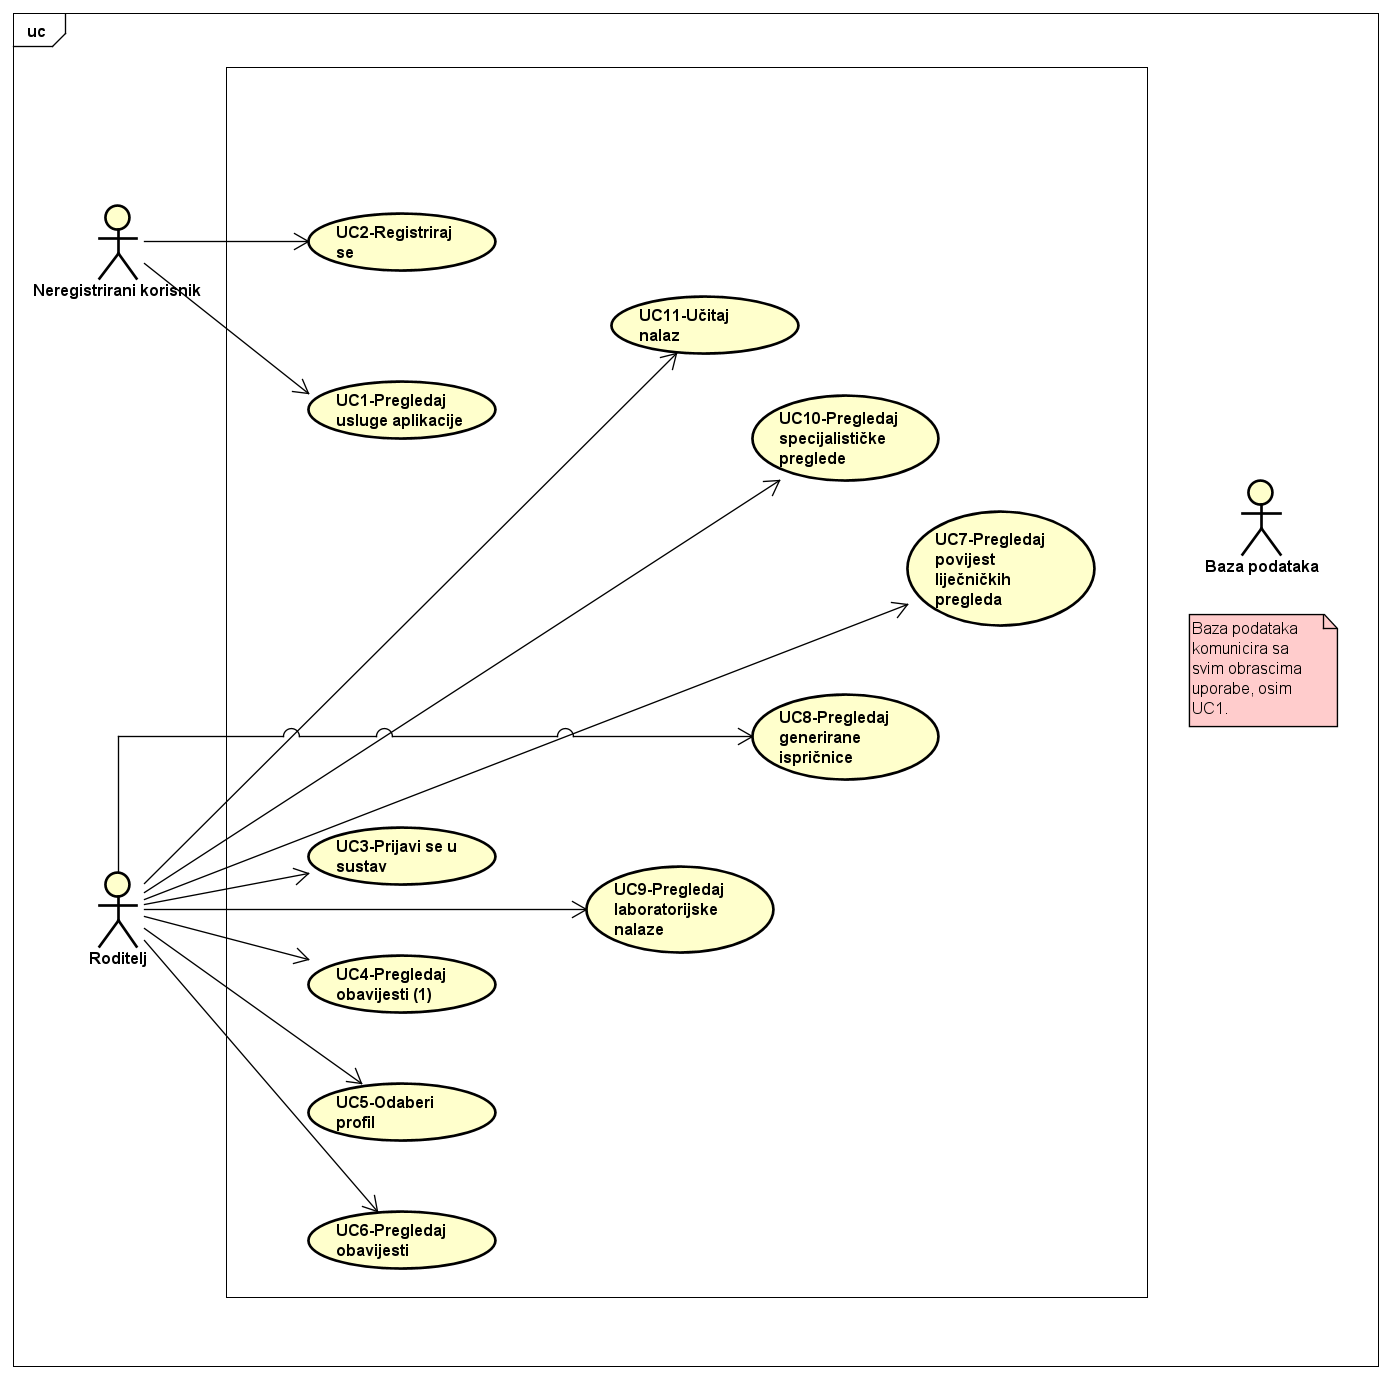
\includegraphics[scale=0.4]{dijagrami/usecase1.PNG} %veličina slike u odnosu na originalnu datoteku i pozicija slike
						\centering
						\caption{Dijagram obrazaca uporabe, funkcionalnost nereg. korisnika i Roditelja}
						\label{fig:useacase1}
					\end{figure}
					
					%unos slike
					\begin{figure}[H]
						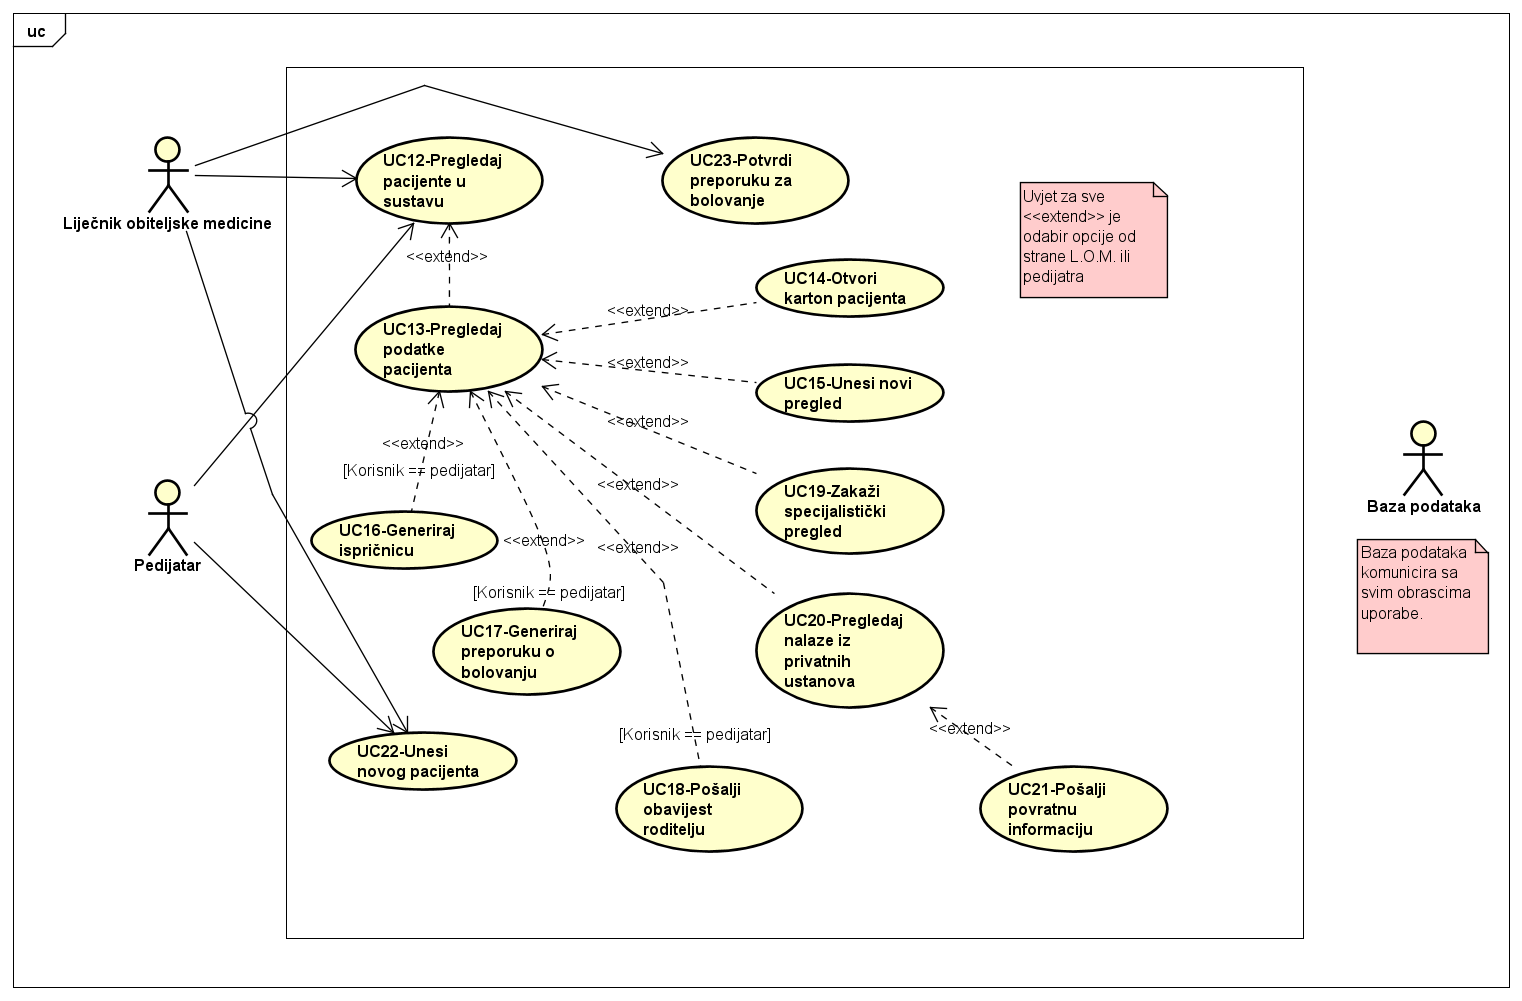
\includegraphics[scale=0.4]{dijagrami/usecase2.PNG} %veličina slike u odnosu na originalnu datoteku i pozicija slike
						\centering
						\caption{Dijagram obrazaca uporabe, funkcionalnost Pedijatra i L.O.M.}
						\label{fig:usecase2}
					\end{figure}
					
					%unos slike
					\begin{figure}[H]
						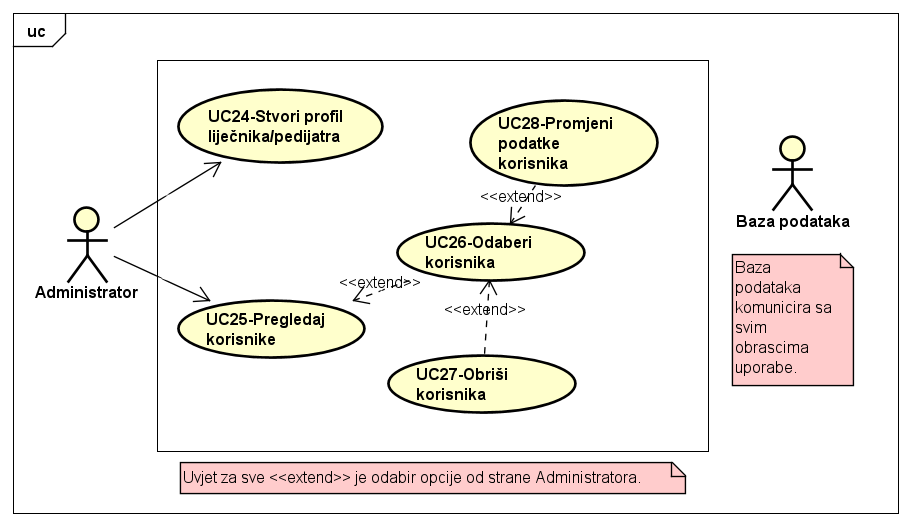
\includegraphics[scale=0.5]{dijagrami/usecase3.PNG} %veličina slike u odnosu na originalnu datoteku i pozicija slike
						\centering
						\caption{Dijagram obrazaca uporabe, funkcionalnost Administratora}
						\label{fig:usecase3}
					\end{figure}
				\eject		
				
			\subsection{Sekvencijski dijagrami}
				\textbf{Sekvencijski dijagram - Obrasci uporabe UC3, UC4, UC5, UC6, UC7 (Od prijave do prikaza povijesti liječničkih pregleda)}\newline
					\text Roditelj prvo šalje zahtjev za prijavom, nakon čega ga sustav prebacuje na ekran za prijavu. Roditelj unosi podatke, koje sustav uzima i provjerava u bazi. Ako su ispravni, sustav dobavlja popis profila vezanih uz korisnički račun i popis svih obavijesti vezanih uz račun roditelja, nakon čega sustav otvara prikaz profila i obavijesti. Kada roditelj odabere jedan od računa, dobavljaju se podaci o tom računu, te popis obavijesti vezanih samo uz taj račun, i zatim se roditelju otvara profil, s prikazanim obavijestima. Roditelj odabire opciju za prikaz povijesti liječničkih pregleda. Sustav nakon toga dobavlja medicinski karton tog profila, nakon čega pomoću identifikatora kartona dobavlja popis obavljenih pregleda. Korisniku se otvara prikaz povijest liječničkih pregleda. \\
					
					%unos slike
					\begin{figure}[H]
						\includegraphics[scale=0.4]{dijagrami/rodseq1.PNG} %veličina slike u odnosu na originalnu datoteku i pozicija slike
						\centering
						\caption{Sekvencijski dijagram prikaza pregleda}
						\label{fig:seq1}
					\end{figure}
					\clearpage
				\textbf{Sekvencijski dijagram - Obrasci uporabe UC13, UC15, UC16 (Odabir pacijenta, novi pregled i ispričnica)}\newline
				\text Na popisu pacijenata pedijatar odabire jednog. Sustav pristupa bazi podataka iz koje vraća podatke o pacijentu, koji se zatim koriste pri stvaranju prikaza osobnih podataka pacijenta. Ako na profilu pacijenta pedijatar odabere opciju za unos novog pregleda, sustav dobavlja podatke o pacijentu ponovno iz baze, te ih zapisuje u polja za podatke pacijenta u prikazu koji stvara za pedijatra. U taj prikaz pedijatar, u za to određena polja, unosi podatke o pregledu. Ti podaci, kao i podaci pacijenta, koriste se u stvaranju novog objekta pregleda koji se sprema u bazu podataka. Pedijatra se nakon potvrde uspješnog spremanja u bazu vraća na profil pacijenta. [Bitno! UC13 i UC15 na identičan način funkcioniraju i za L.O.M.] Ako pedijatar odabere opciju za generiranje ispričnice, sustav iz baze prenosi podatak o kontaktu škole, koji se zapisuje u polje u prikazu za stvaranje nove ispričnice. U tom prikazu pedijatar ispunjava ostala polja, primarno opis razloga izdavanja ispričnice. Ispričnica se generira, prilikom čega se prvo šalje školi, a zatim sprema u bazu. Nakon primljene potvrde o uspješnom spremanju u bazu, sustav vraća pedijatra na profil pacijenta.
				
				%unos slike
				\begin{figure}[H]
					\includegraphics[scale=0.35]{dijagrami/pedseq1.PNG} %veličina slike u odnosu na originalnu datoteku i pozicija slike
					\centering
					\caption{Sekvencijski dijagram osnovnih funkcionalnosti pedijatra}
					\label{fig:seq2}
				\end{figure}
				\clearpage
				
				\textbf{Sekvencijski dijagram - Obrasci uporabe UC17 i UC23 (Generiranje i potvrda preporuke o bolovanju)}\newline
					\text Na profilu pacijenta pedijatar odabire opciju generiraj preporuku za bolovanje. Sustav iz baze podataka dohvaća podatke o roditelju pacijenta. Iz njih se čuvaju email adresa poslodavca i identifikator liječnika. Pedijatru se otvara prikaz u kojem ispunjava podatke o preporuci o bolovanju (npr. razlog i trajanje, te ime i prezime roditelja). Nakon potvrde generiranja preporuke, ona se sprema u bazu podataka.
					Kada liječnik želi pristupiti preporukama o bolovanju, on odabire opciju na svom izborniku. Kada odabere tu opciju, iz baze se dohvaćaju sve preporuke o bolovanju koje su povezane na doktora putem njegovog identifikatora. Za svaku doktor može odabrati opciju "Potvrdi" ili "Odbij". Prilikom potvrde se generira i šalje doznaka o bolovanju poslodavcu, nakon čega se preporuka briše iz baze. U slučaju odbijanja, preporuka se isto briše iz baze, bez slanja.
					%unos slike
					\begin{figure}[H]
						\includegraphics[scale=0.4]{dijagrami/pedseq2.PNG} %veličina slike u odnosu na originalnu datoteku i pozicija slike
						\centering
						\caption{Sekvencijski dijagram stvaranja i potvrde preporuke o bolovanju}
						\label{fig:seq3}
					\end{figure}
					\clearpage
					
				\textbf{Sekvencijski dijagram - Obrasci uporabe UC11, UC20 i UC21 (\textit{Upload} nalaza, pregled svih nalaza i opcionalno slanje povratne informacije)}\newline
					\text Roditelj može na meniju otvorenog profila odabrati opciju za učitavanje nalaza od privatnika. Sustav roditelju otvara prikaz za \textit{upload} s poljima za dodatne informacije. Nakon što roditelj odabire opciju "Učitaj", stvara se novi objekt privatnog nalaza, koji se povezuje na medicinski karton pacijenta, čiji je identifikator jedno od polja u objektu Roditelj/Dijete. Pedijatar/liječnik može na otvorenom profilu pacijenta odabrati opciju za prikaz nalaza od privatnika. U tom slučaju sustav iz baze podataka dobavlja popis, i prikazuje ga pedijatru/liječniku, nakon čega pedijatar/liječnik može otvoriti svaki pojedinačno. Nakon otvaranja detaljnog prikaza nalaza, pedijatar može odabrati opciju za slanje povratne informacije. Nakon toga mu sustav otvara prikaz za slanje obavijesti. Nakon ispunjavanja podataka obavijesti i pritiska opcije za slanje, sustav dobavlja OIB koji je potreban za stvaranje objekta obavijesti iz baze, nakon čega sprema obavijest. [Važno: postupak čitanja obavijesti već je opisan u sekvencijskom dijagramu (Slika 3.4)]
					%unos slike
					\begin{figure}[H]
						\includegraphics[scale=0.4]{dijagrami/pedseq3.PNG} %veličina slike u odnosu na originalnu datoteku i pozicija slike
						\centering
						\caption{Sekvencijski dijagram rada s privatnim nalazima}
						\label{fig:seq4}
					\end{figure}
					\clearpage
				
					
				\eject
	
		\section{Ostali zahtjevi}
			 
			 \text Aplikacija treba biti prilagođena radu na različitim uređajima, specifično na računalima, tabletima i mobitelima. \\
			 \text Aplikacija treba podržavati više korisnika u isto vrijeme. Maksimalan broj podržanih korisnika nije definiran. \\
			 \text Aplikacija treba biti izvedena kao web aplikacija. Siguran pristup mora biti osiguran korisničkim imenom i lozinkom, no nisu definirani zahtjevi dodatne zaštite.
			 
			 
			 
	
	\chapter{Arhitektura i dizajn sustava}
		
		\text	Arhitektura našeg projekta podijeljena je na tri generalna dijela:
		\begin{packed_item}
			\item Web poslužitelj
			\item Web aplikacija
			\item Baza podataka
		\end{packed_item}
		
		%unos slike
		\begin{figure}[H]
			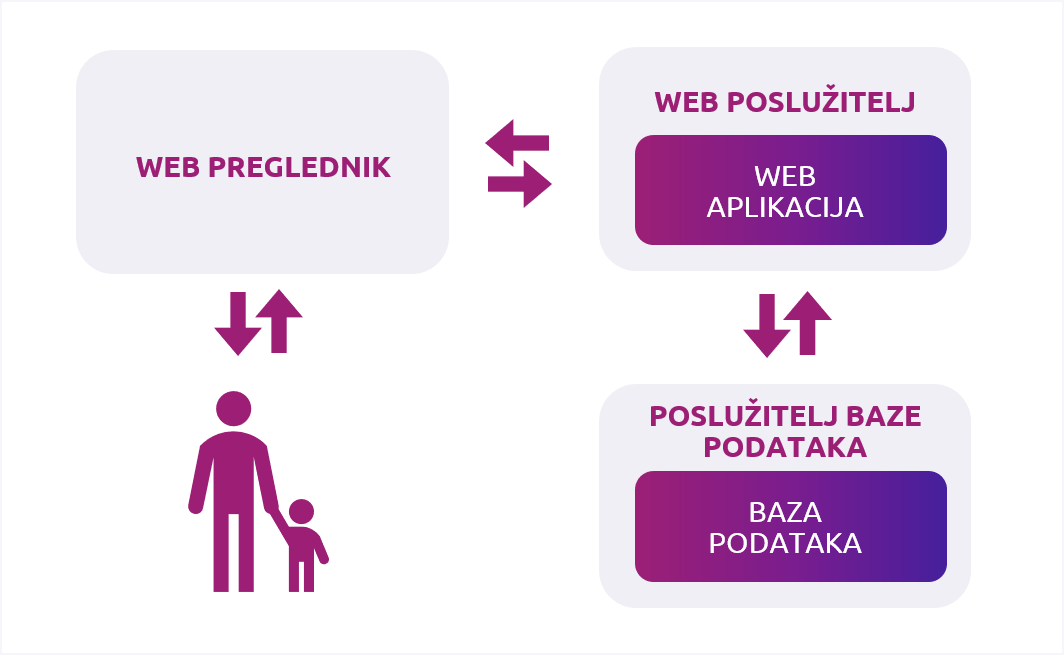
\includegraphics[scale=0.4]{slike/graf1b.PNG} %veličina slike u odnosu na originalnu datoteku i pozicija slike
			\centering
			\caption{Dijagram arhitekture projekta}
			\label{fig:arhitektura-sustava}
		\end{figure}
		
		\text	Web preglednik je program koji omogućava korisnicima pregledavanje web-stranica i multimedijskih sadržaja, te interakciju s njima. Svaki web preglednik također je i svojevrsni prevoditelj, koji programski kod otvorenih stranica interpretira u razumljivi format za korisnike. Kada korisnik koristi web aplikacije, njegovi zahtjevi šalju se putem web preglednika prema web poslužitelju. \\
		\\
		\text	Web poslužitelj glavni je dio zadužen za rad aplikacije. S njime korisnik komunicira s web aplikacijom. Ta komunikacija vrši se putem HTTP protokola (engl. \textit{Hyper Text Transfer Protokol}). Web poslužitelj također je zadužen za pokretanje web aplikacije, nakon čega joj šalje korisničke zahtjeve. \\
		\\
		\text	Web aplikacija obrađuje korisničke zahtjeve, prilikom čega pristupa bazi podataka. Obrađene podatke vraća korisniku putem poslužitelja, koji zatim navedene podatke prikazuje u web pregledniku. \\
		\\
		\text	Prilikom razvoja ovog projekta, koristili smo programski jezik Java i alat \textit{Spring Boot} za razvoj web aplikacije. Za razvoj izgleda kakav se prikazuje u web pregledniku koristili smo programski jezik Java-Script i Java-Script biblioteku \textit{React}. Razvoj projekta vršio se u razvojnom okruženju \textit{IntelliJ IDEA}.  \\
		\\
		\text	Za razvoj našeg projekta odlučili smo se ugledati na MVC [Model-Pogled-Nadglednik] (engl. \textit{Model-View-Controller}) koncept arhitekture sustava. Glavna karakteristika imenovanog koncepta jest smanjena međuovisnost korisničkog sučelja i ostatka sustava. Takav koncept omogućava lakše testiranje i daljnji razvoj sustava.
		\begin{packed_item}
			\item \textbf{Model} - Središnji dio cijelog sustava. Sadrži razrede čiji se objekti/podaci obrađuju. Izravno upravlja s podacima i pravilima aplikacije.
			\item \textbf{Pogled} - Sadrži razrede čiji objekti služe za prikaz podataka, u bilo kojem obliku.
			\item \textbf{Nadglednik} - Sadrži razrede koji upravljaju i rukuju korisničkom interakcijom s pogledom i modelom. 
		\end{packed_item}
		\text	Također smo se u našem kodu odlučili koristiti \textit{Controller-Service-Repository} uzorkom koji je dosta čest u aplikacijama koje koriste \textit{Spring Boot} alat. On se, očito iz naziva, sastoji od tri dijela:
		\begin{packed_item}
			\item \textbf{Controller} - "Najviši" dio. Služi za bilo kakvu interakciju između okoline aplikacije i njene unutarnje logike.
			\item \textbf{Service} - "Središnji" dio. Unutar njega se implementiraju sve funkcije i sva logika aplikacije. 
			\item \textbf{Repository} - "Najniži" dio. Služi za spremanje entiteta unutar sustava. Može imati vlastite funkcije, ali njih poziva \textit{Service}. 
		\end{packed_item}
		\clearpage
		
		
		

				
		\section{Baza podataka}
			
			\text Za potrebe našeg projekta koristili smo relacijsku bazu podataka napisanu u programskom jeziku Java, pokrenutu \textit{engine-om} H2. Prednost te vrste baze podataka jest jednostavnost modeliranja pravog svijeta na temelju relacija. Zadaća baze podataka u projektu jest pohrana, izmjena i dohvat podataka koji se zatim obrađuju. Baza podataka sastoji se od entiteta:
			\begin{packed_item}
				\item Roditelj
				\item Dijete
				\item Pedijatar
				\item Liječnik obiteljske medicine
				\item Medicinski karton
				\item Pregled
				\item Nalaz
				\item Obavijest
				\item Specijalistički pregled
				\item Preporuka o bolovanju
				\item Ispričnica
			\end{packed_item}
		
			\subsection{Opis tablica}
			

				\textbf{Roditelj} - Entitet sadržava sve podatke koje roditelj unosi prilikom registracije. Oni su: OIB, ime i prezime, datum rođenja, korisničko ime, lozinka, broj telefona, e-mail, poštanski broj, mjesto prebivališta, e-mail poslodavca te šifra liječnika. Entitet roditelj u odnosu je \textit{Many-to-One} s entitetom Liječnik obiteljske medicine preko šifre tog liječnika, u odnosu \textit{One-to-Many} sa entitetom Dijete, putem vlastitog OIB-a, te u odnosu \textit{One-to-One} s entitetom Medicinski karton, putem jedinstvenog identifikatora kartona.
				
				
				\begin{longtblr}[
					label=none,
					entry=none
					]{
						width = \textwidth,
						colspec={|X[10,l]|X[6, l]|X[20, l]|}, 
						rowhead = 1,
					} %definicija širine tablice, širine stupaca, poravnanje i broja redaka naslova tablice
					\hline \SetCell[c=3]{c}{\textbf{Parent/Roditelj}}	 \\ \hline[3pt]
					\SetCell{LightGreen}OIB & CHAR(11)	&  	Jedinstveni identifikator roditelja	\\ \hline
					nameParent	& VARCHAR &   Ime roditelja	\\ \hline 
					lastNameParent	& VARCHAR &   Prezime roditelja	\\ \hline 
					dateOfBirthParent	& DATE &  Datum rođenja roditelja 	\\ \hline 
					userNameParent	& VARCHAR &   Korisničko ime računa	\\ \hline 
					passwordParent	& VARCHAR &   Zaporka računa	\\ \hline 
					phoneNumberParent	& VARCHAR &   Broj telefona roditelja	\\ \hline 
					emailParent	& VARCHAR &   E-mail roditelja	\\ \hline 
					postalCode & INT &  Poštanski broj mjesta stanovanja \\ \hline 
					placeOfResidence & VARCHAR	&  	Mjesto stanovanja roditelja	\\ \hline 
					employerEmail	& VARCHAR &   E-mail poslodavca roditelja	\\ \hline 
					\SetCell{LightBlue}doctorId	& INT &   Identifikator L.O.M.-a roditelja	\\ \hline
					\SetCell{LightBlue}recordId	& INT &   Identifikator medicinskog kartona roditelja	\\ \hline
				\end{longtblr}
				
				\textbf{Dijete} - Entitet sadržava sve podatke koje unosi pedijatar prilikom prvog pregleda djeteta. Oni su: OIB, OIB roditelja, šifra pedijatra, ime i prezime, datum rođenja, naziv škole/vrtića te e-mail škole/vrtića. Entitet dijete u odnosu je \textit{Many-to-One} sa entitetom Roditelj, putem roditeljevog OIB-a, u odnosu \textit{Many-to-One} s entitetom Pedijatar putem pedijatrovog ID-a, te u odnosu \textit{One-to-One} s entitetom Medicinski karton, putem jedinstvenog identifikatora kartona.
				
				\begin{longtblr}[
					label=none,
					entry=none
					]{
						width = \textwidth,
						colspec={|X[11,l]|X[6, l]|X[20, l]|}, 
						rowhead = 1,
					} %definicija širine tablice, širine stupaca, poravnanje i broja redaka naslova tablice
					\hline \SetCell[c=3]{c}{\textbf{Child/Dijete}}	 \\ \hline[3pt]
					\SetCell{LightGreen}OIB & CHAR(11)	&  	Jedinstveni identifikator djeteta 	\\ \hline
					nameChild	& VARCHAR &   Ime djeteta	\\ \hline 
					lastNameChild	& VARCHAR &   Prezime djeteta	\\ \hline 
					dateOfBirthChild	& DATE &   Datum rođenja djeteta	\\ \hline 
					educationalInstitution	& VARCHAR &   Ime škole/vrtića djeteta	\\ \hline 
					emailEduInstitution & VARCHAR &  E-mail škole/vrtića \\ \hline 
					\SetCell{LightBlue} pediatricanId	& INT &   Jedinstveni identifikator pedijatra	\\ \hline 
					\SetCell{LightBlue}recordId	& INT &   Identifikator medicinskog kartona djeteta	\\ \hline
					\SetCell{LightBlue}parentOib & CHAR(11)	&  Jedinstveni identifikator roditelja	\\ \hline 
				\end{longtblr}
				
				\textbf{Pedijatar} - Entitet sadržava sve podatke koje unosi administrator prilikom registracije pedijatra u sustav. Oni su: šifra pedijatra, ime i prezime, datum rođenja, korisničko ime, lozinka, broj telefona, e-mail. Entitet pedijatar u odnosu je \textit{One-to-Many} s entitetom Dijete putem vlastite šifre.
				
				\begin{longtblr}[
					label=none,
					entry=none
					]{
						width = \textwidth,
						colspec={|X[12,l]|X[6, l]|X[20, l]|}, 
						rowhead = 1,
					} %definicija širine tablice, širine stupaca, poravnanje i broja redaka naslova tablice
					\hline \SetCell[c=3]{c}{\textbf{Pediatrician/Pedijatar}}	 \\ \hline[3pt]
					\SetCell{LightGreen}pediatricianId & INT	&  	Jedinstveni identifikator pedijatra	\\ \hline
					namePediatirican	& VARCHAR &   Ime pedijatra	\\ \hline 
					lastNamePediatirican	& VARCHAR &   Prezime pedijatra	\\ \hline 
					dateOfBirthPediatirican	& DATE &   Datum rođenja pedijatra	\\ \hline 
					userNamePediatirican	& VARCHAR &   Korisničko ime računa	\\ \hline 
					passwordPediatrician & VARCHAR &  Zaporka računa \\ \hline 
					phoneNumPediatrician	& VARCHAR &   Broj telefona pedijatra	\\ \hline 
					emailPediatrician	& VARCHAR &   E-mail pedijatra	\\ \hline
					
				\end{longtblr}
				
				\textbf{Liječnik obiteljske medicine} - Entitet sadržava sve podatke koje unosi administrator prilikom registracije LOM-a u sustav. Oni su: šifra doktora, ime i prezime, datum rođenja, korisničko ime, lozinka, broj telefona i e-mail. Entitet Liječnik obiteljske medicine u odnosu je \textit{One-to-Many} s entitetom Roditelj putem vlastite šifre.
				
				\begin{longtblr}[
					label=none,
					entry=none
					]{
						width = \textwidth,
						colspec={|X[10,l]|X[6, l]|X[20, l]|}, 
						rowhead = 1,
					} %definicija širine tablice, širine stupaca, poravnanje i broja redaka naslova tablice
					\hline \SetCell[c=3]{c}{\textbf{Doctor/Liječnik obiteljske medicine}}	 \\ \hline[3pt]
					\SetCell{LightGreen}doctorId & INT	&  	Jedinstveni identifikator liječnika	\\ \hline
					nameDoctor	& VARCHAR &   Ime liječnika	\\ \hline 
					lastNameDoctor	& VARCHAR &   Prezime liječnika	\\ \hline 
					dateOfBirthDoctor	& DATE &   Datum rođenja liječnika	\\ \hline 
					userNameDoctor	& VARCHAR &   Korisničko ime računa	\\ \hline 
					passwordDoctor & VARCHAR &  Zaporka računa \\ \hline 
					phoneNumDoctor	& VARCHAR &   Broj telefona liječnika	\\ \hline 
					emailDoctor	& VARCHAR &   E-mail liječnika	\\ \hline
					
				\end{longtblr}
				
				\textbf{Medicinski karton} - Entitet sadržava podatke za opis medicinskog kartona pojedinog pacijenta (roditelj/dijete). Oni su: šifra kartona, OIB, trenutna dijagnoza i popis alergija. Entitet Medicinski karton u odnosu je \textit{One-to-One} s entitetom Roditelj i s entitetom Dijete, putem vlastitog jedinstvenog identifikatora, te u odnosima \textit{One-to-Many} s entitetima Nalaz i Pregled.  
				
				\begin{longtblr}[
					label=none,
					entry=none
					]{
						width = \textwidth,
						colspec={|X[8,l]|X[6, l]|X[20, l]|}, 
						rowhead = 1,
					} %definicija širine tablice, širine stupaca, poravnanje i broja redaka naslova tablice
					\hline \SetCell[c=3]{c}{\textbf{MedicalRecord/Medicinski karton}}	 \\ \hline[3pt]
					\SetCell{LightGreen}redordId & INT	&  	Jedinstveni identifikator kartona	\\ \hline
					currentDiagnosis & VARCHAR &  Aktivna ili zadnja dijagnoza djeteta \\ \hline 
					allergyList & VARCHAR	&  	Popis alergija djeteta	\\ \hline
				\end{longtblr}
				
				\textbf{Pregled} - Entitet sadržava podatke pregleda kojeg održava pedijatar ili LOM. Oni su: šifra pregleda, šifra kartona kojem pripada, dijagnoza i datum pregleda. Entitet Pregled u odnosu je \textit{Many-to-One} s entitetom Medicinski karton.
				
				\begin{longtblr}[
					label=none,
					entry=none
					]{
						width = \textwidth,
						colspec={|X[9,l]|X[6, l]|X[20, l]|}, 
						rowhead = 1,
					} %definicija širine tablice, širine stupaca, poravnanje i broja redaka naslova tablice
					\hline \SetCell[c=3]{c}{\textbf{Examination/Pregled}}	 \\ \hline[3pt]
					\SetCell{LightGreen}examinationId & INT	&  	Jedinstveni identifikator pregleda	\\ \hline
					\SetCell{LightBlue}recordId	& INT &  Jedinstveni identifikator kartona 	\\ \hline 
					diagnosis & VARCHAR &  Opis dijagnoze  \\ \hline 
					dateOfExamination & DATE	&  	Datum pregleda	\\ \hline
				\end{longtblr}
				
				\textbf{Nalaz} - Entitet sadržava podatke koji opisuju nalaz dobiven prilikom privatnog pregleda, kojeg \textit{uploada} roditelj. Oni su: šifra nalaza, šifra kartona, datum nalaza, podaci nalaza. Entitet Nalaz u odnosu je \textit{Many-to-One} s entitetom Medicinski karton.
				
				\begin{longtblr}[
					label=none,
					entry=none
					]{
						width = \textwidth,
						colspec={|X[9,l]|X[6, l]|X[20, l]|}, 
						rowhead = 1,
					} %definicija širine tablice, širine stupaca, poravnanje i broja redaka naslova tablice
					\hline \SetCell[c=3]{c}{\textbf{MedicalReport/Nalaz}}	 \\ \hline[3pt]
					\SetCell{LightGreen}reportId & INT	&  	Jedinstveni identifikator nalaza	\\ \hline
					\SetCell{LightBlue}recordId	& INT &  Jedinstveni identifikator kartona 	\\ \hline 
					reportInformation & VARCHAR &  Podaci iz nalaza  \\ \hline 
					dateOfReport & DATE	&  	Datum pregleda	\\ \hline
				\end{longtblr}
				
				\textbf{Obavijest} - Entitet sadržava podatke koji opisuju obavijest poslanu roditelju, koju piše liječnik/pedijatar. Oni su: šifra obavijesti, OIB roditelja, OIB djeteta, naslov i tekst obavijesti. Entitet Obavijest u odnosu je \textit{Many-to-One} s entitetima Roditelj i Dijete.
				
				\begin{longtblr}[
					label=none,
					entry=none
					]{
						width = \textwidth,
						colspec={|X[11,l]|X[6, l]|X[20, l]|}, 
						rowhead = 1,
					} %definicija širine tablice, širine stupaca, poravnanje i broja redaka naslova tablice
					\hline \SetCell[c=3]{c}{\textbf{Notification/Obavijest}}	 \\ \hline[3pt]
					\SetCell{LightGreen}notificationId & INT	&  	Jedinstveni identifikator obavijesti	\\ \hline
					\SetCell{LightBlue}parentOib	& CHAR(11) &  Jedinstveni identifikator roditelja 	\\ \hline 
					\SetCell{LightBlue}childOib	& CHAR(11) &  Jedinstveni identifikator djeteta	\\ \hline 
					notificationInformation & VARCHAR &  Podaci obavijesti  \\ \hline 
					notificationTitle & VARCHAR &  Naslov obavijesti  \\ \hline 
				\end{longtblr}
				
				\textbf{Specijalistički pregled} - Entitet sadržava podatke koji opisuju specijalistički pregled na kojeg liječnik/pedijatar prijavljuje pacijenta. Oni su: šifra pregleda, šifra pacijenta, naziv pregleda, moguće lokacije pregleda. Entitet Spec. pregled u odnosu je \textit{Many-to-One} s entitetom Medicinski karton, preko čega mu pristupaju entiteti Roditelj i Dijete.
				
				\begin{longtblr}[
					label=none,
					entry=none
					]{
						width = \textwidth,
						colspec={|X[9,l]|X[6, l]|X[20, l]|}, 
						rowhead = 1,
					} %definicija širine tablice, širine stupaca, poravnanje i broja redaka naslova tablice
					\hline \SetCell[c=3]{c}{\textbf{SpecialistExamination/Specijalistički pregled}}	 \\ \hline[3pt]
					\SetCell{LightGreen}examId & INT	&  	Jedinstveni identifikator pregleda	\\ \hline
					\SetCell{LightBlue}recordId	& INT &  Jedinstveni identifikator kartona	\\ \hline 
					examTitle & VARCHAR &  Naziv pregleda  \\ \hline 
					examLocations & VARCHAR	&  	Moguće lokacije pregleda	\\ \hline
				\end{longtblr}
				
				\textbf{Preporuka o bolovanju} - Entitet sadržava podatke o bolovanju kojeg pedijatar preporučuje za roditelja djeteta. Oni su: šifra preporuke, šifra liječnika obiteljske medicine, opis razloga za bolovanje i trajanja, te email poslodavca. Entitet Preporuka o bolovanju u odnosu je \textit{Many-to-One} s entitetom Liječnik obiteljske medicine.
				
				\begin{longtblr}[
					label=none,
					entry=none
					]{
						width = \textwidth,
						colspec={|X[9,l]|X[6, l]|X[20, l]|}, 
						rowhead = 1,
					} %definicija širine tablice, širine stupaca, poravnanje i broja redaka naslova tablice
					\hline \SetCell[c=3]{c}{\textbf{SickLeaveRecommendation/Preporuka o bolovanju}}	 \\ \hline[3pt]
					\SetCell{LightGreen}recommendationId & INT	&  	Jedinstveni identifikator preporuke	\\ \hline
					\SetCell{LightBlue}doctorId	& INT &  Jedinstveni identifikator liječnika	\\ \hline 
					recData & VARCHAR &  Sadržaj preporuke  \\ \hline
					employerEmail & VARCHAR &  email poslodavca kojem se šalje doznaka  \\ \hline
				\end{longtblr}
				
				\textbf{Ispričnica} - Entitet sadržava podatke o ispričnici koju pedijatar piše za dijete. Oni su: šifra ispričnice, OIB djeteta, opis razloga za ispričnicom i trajanja. Entitet Ispričnica u odnosu je \textit{Many-to-One} s entitetom Dijete.
				
				\begin{longtblr}[
					label=none,
					entry=none
					]{
						width = \textwidth,
						colspec={|X[9,l]|X[6, l]|X[20, l]|}, 
						rowhead = 1,
					} %definicija širine tablice, širine stupaca, poravnanje i broja redaka naslova tablice
					\hline \SetCell[c=3]{c}{\textbf{SickNote/Ispričnica}}	 \\ \hline[3pt]
					\SetCell{LightGreen}sicknoteId & INT	&  	Jedinstveni identifikator ispričnice	\\ \hline
					\SetCell{LightBlue}childOib	& CHAR(11) &  Jedinstveni identifikator djeteta	\\ \hline 
					noteData & VARCHAR &  Sadržaj ispričnice  \\ \hline
				\end{longtblr}
			\subsection{Dijagrami baze podataka}
				%unos slike
				\begin{figure}[H]
					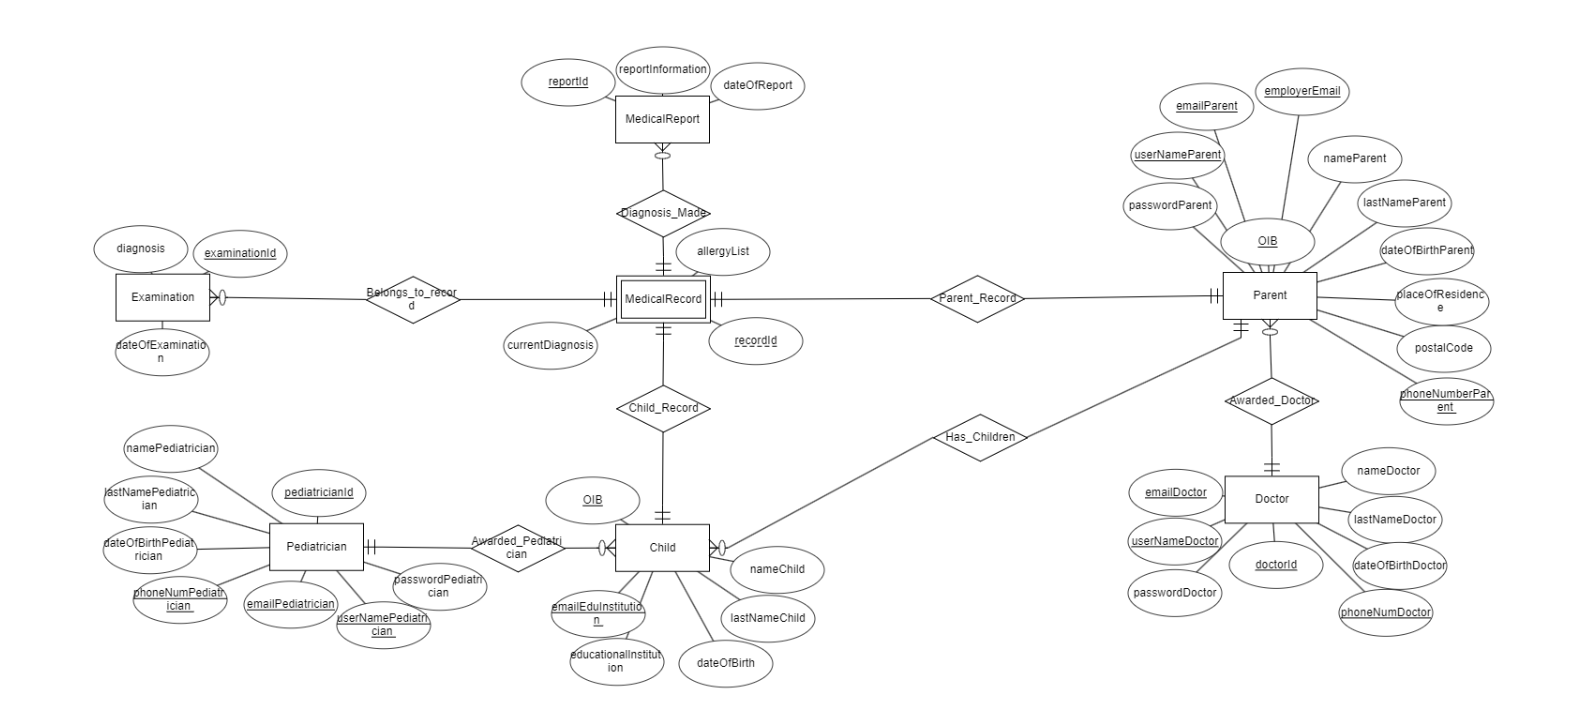
\includegraphics[scale=0.1]{dijagrami/ozdraviER.PNG} %veličina slike u odnosu na originalnu datoteku i pozicija slike
					\centering
					\caption{Dijagram arhitekture baze podataka}
					\label{fig:arhitektura-baze1}
				\end{figure}
				
				%unos slike
				\begin{figure}[H]
					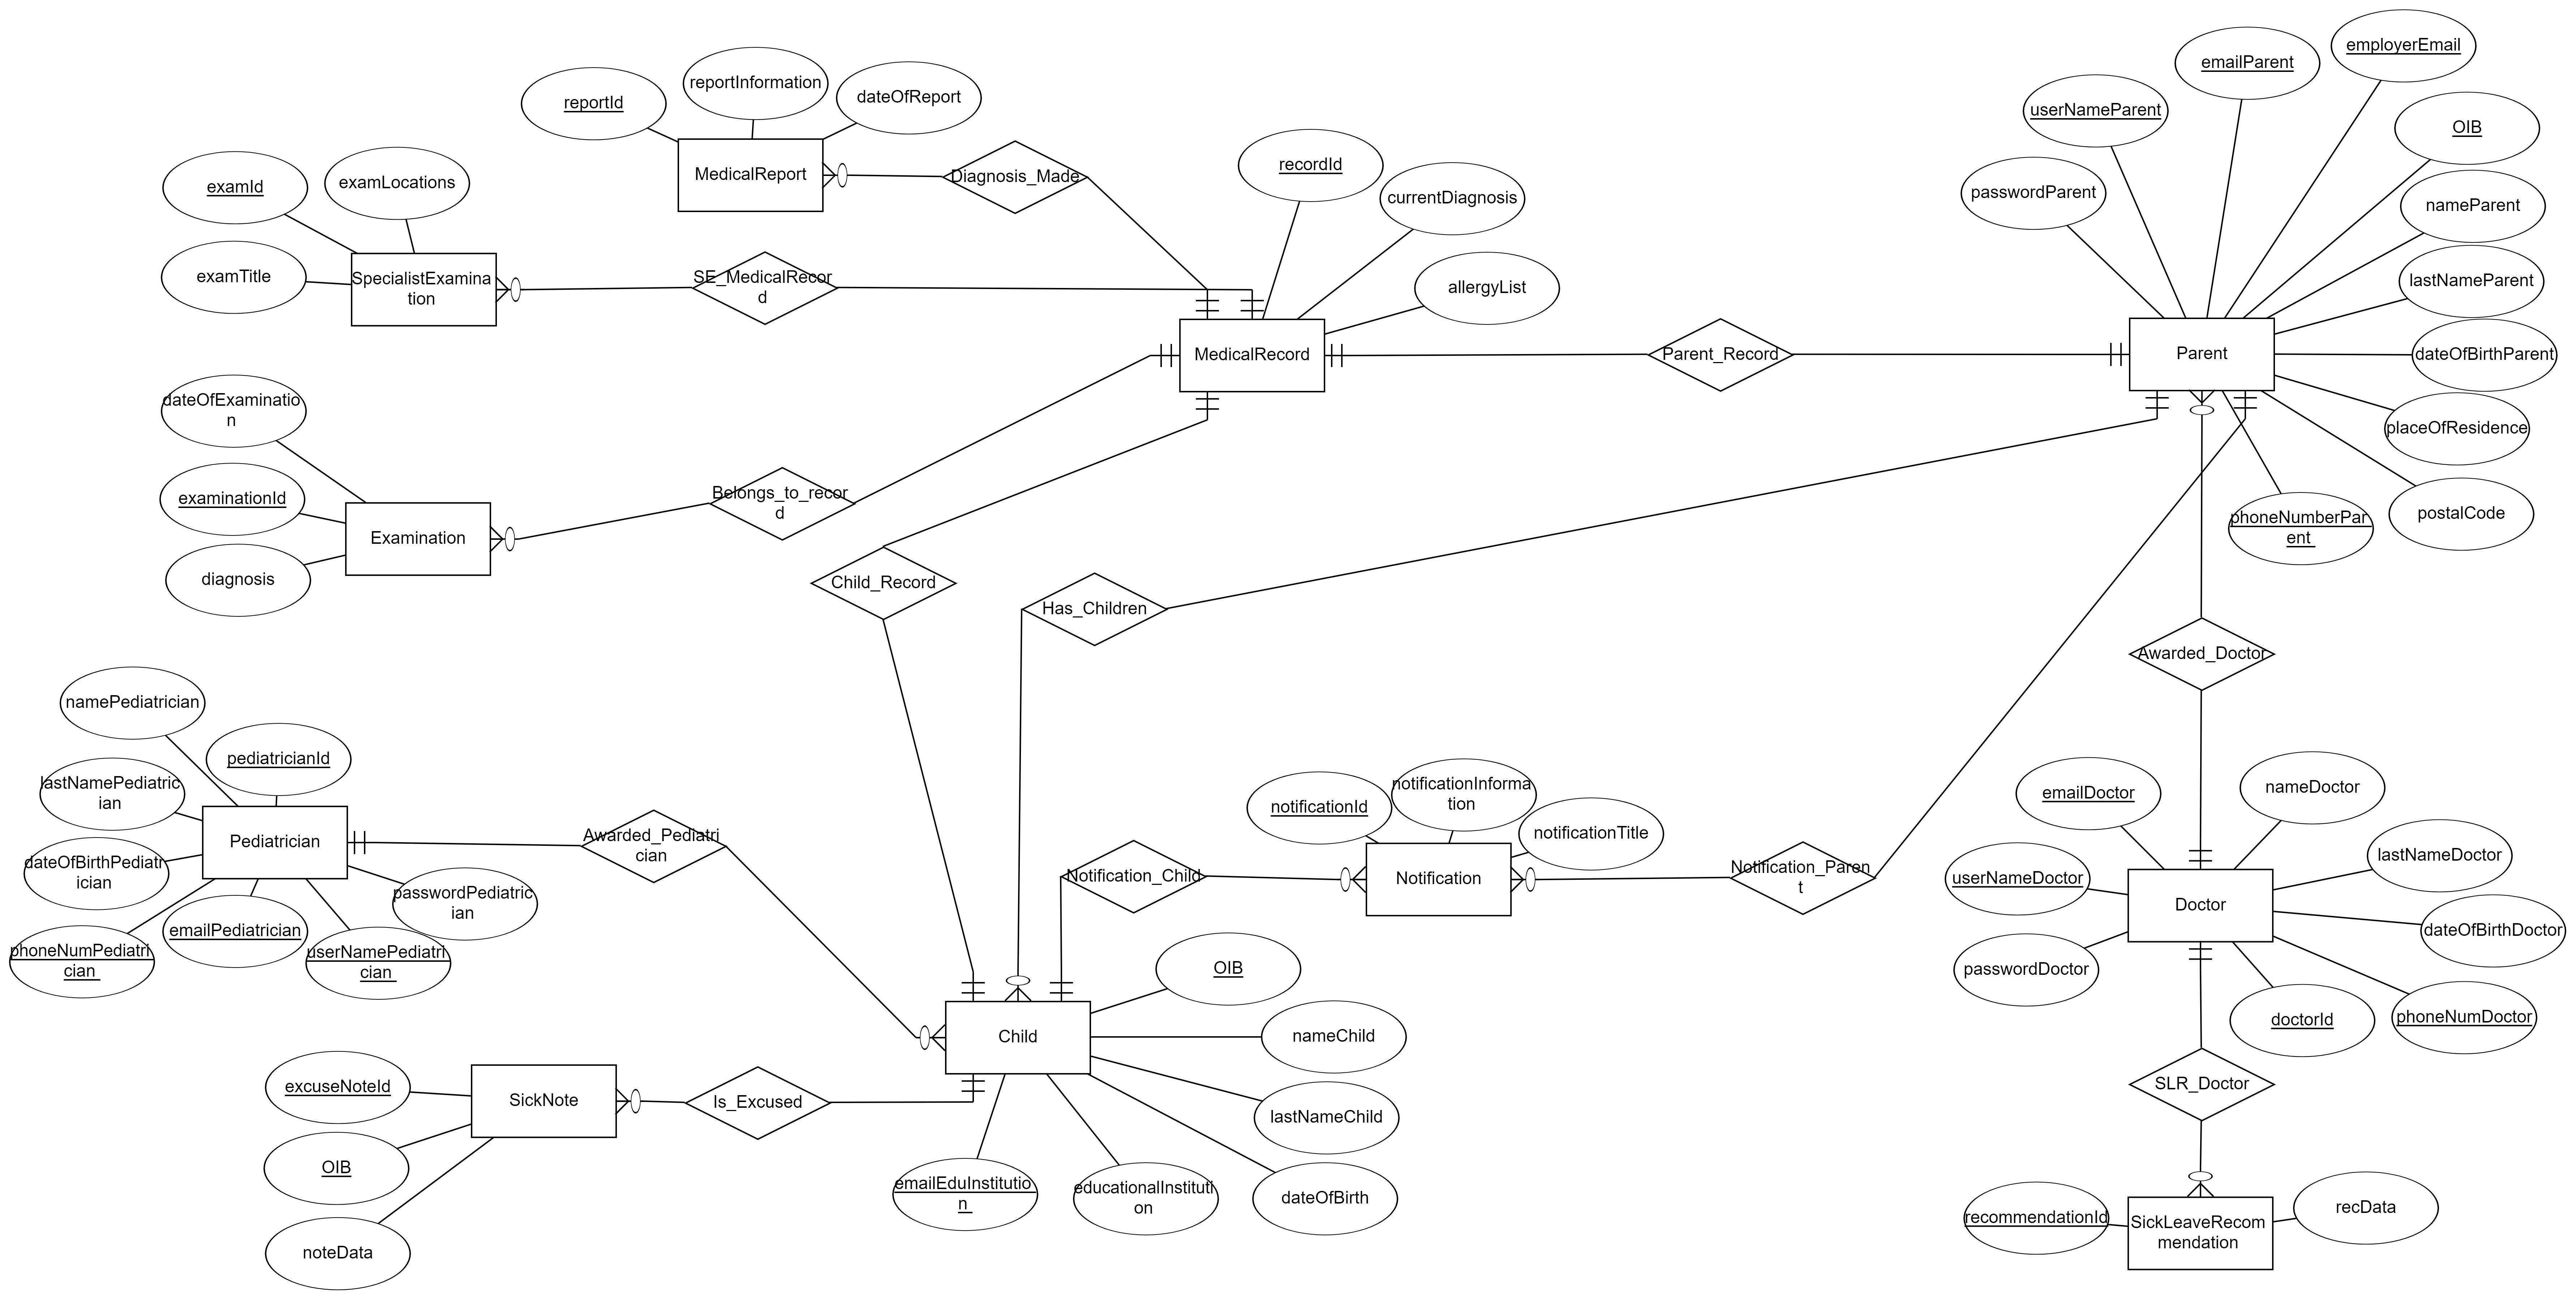
\includegraphics[scale=0.07]{dijagrami/ozdraviREL.PNG} %veličina slike u odnosu na originalnu datoteku i pozicija slike
					\centering
					\caption{Dijagram arhitekture baze podataka}
					\label{fig:arhitektura-baze2}
				\end{figure}
				\clearpage
			\eject
			
		\section{Dijagram razreda}
		
			\text Na sljedećim slikama prikazani su dijagrami razreda ovog projekta. Zbog lakšeg snalaženja, razredi su raspodijeljeni na nekoliko dijagrama.\\
			Postoje četiri razreda koji označavaju osobu: liječnik obiteljske medicine (Doctor), pedijatar (Pediatrician), roditelj (Parent) i njegovo dijete (Child). Razred Parent predstavlja roditelja koji se registrira u sustav te povezuje svoju djecu radi komunikacije s pedijatrom i liječnikom. Razred Doctor predstavlja liječnika obiteljske medicine kojeg registrira administrator i ima komunikaciju s roditeljem u vezi bolovanja, te ostalim zadaćama liječnika i pacijenta. Razred Pediatrician predstavlja pedijatra koji je zadužen za liječenje djeteta i izdavanje ispričnica i medicinskih dokumentacija. Razred Child predstavlja dijete registriranog roditelja koje se liječi kod pedijatra. Za dijete i roditelja kao pacijente vežu se tri razreda koji označavaju vrstu medicinske dokumentacije: medicinski kartoni (MedicalRecord), pregledi (Examination), specijalistički pregledi (SpecialistExamination) i nalazi (MedicalReport). Pregledi i nalazi su s djetetom povezani preko medicinskog kartona. Liječnik je povezan s roditeljem, a pedijatar je povezan s roditeljem preko djeteta. Razredi RegistrationRequest i LoginRequest služe za registraciju i prijavu korisnika u sustav.
				 
			
			%unos slike
			\begin{figure}[H]
				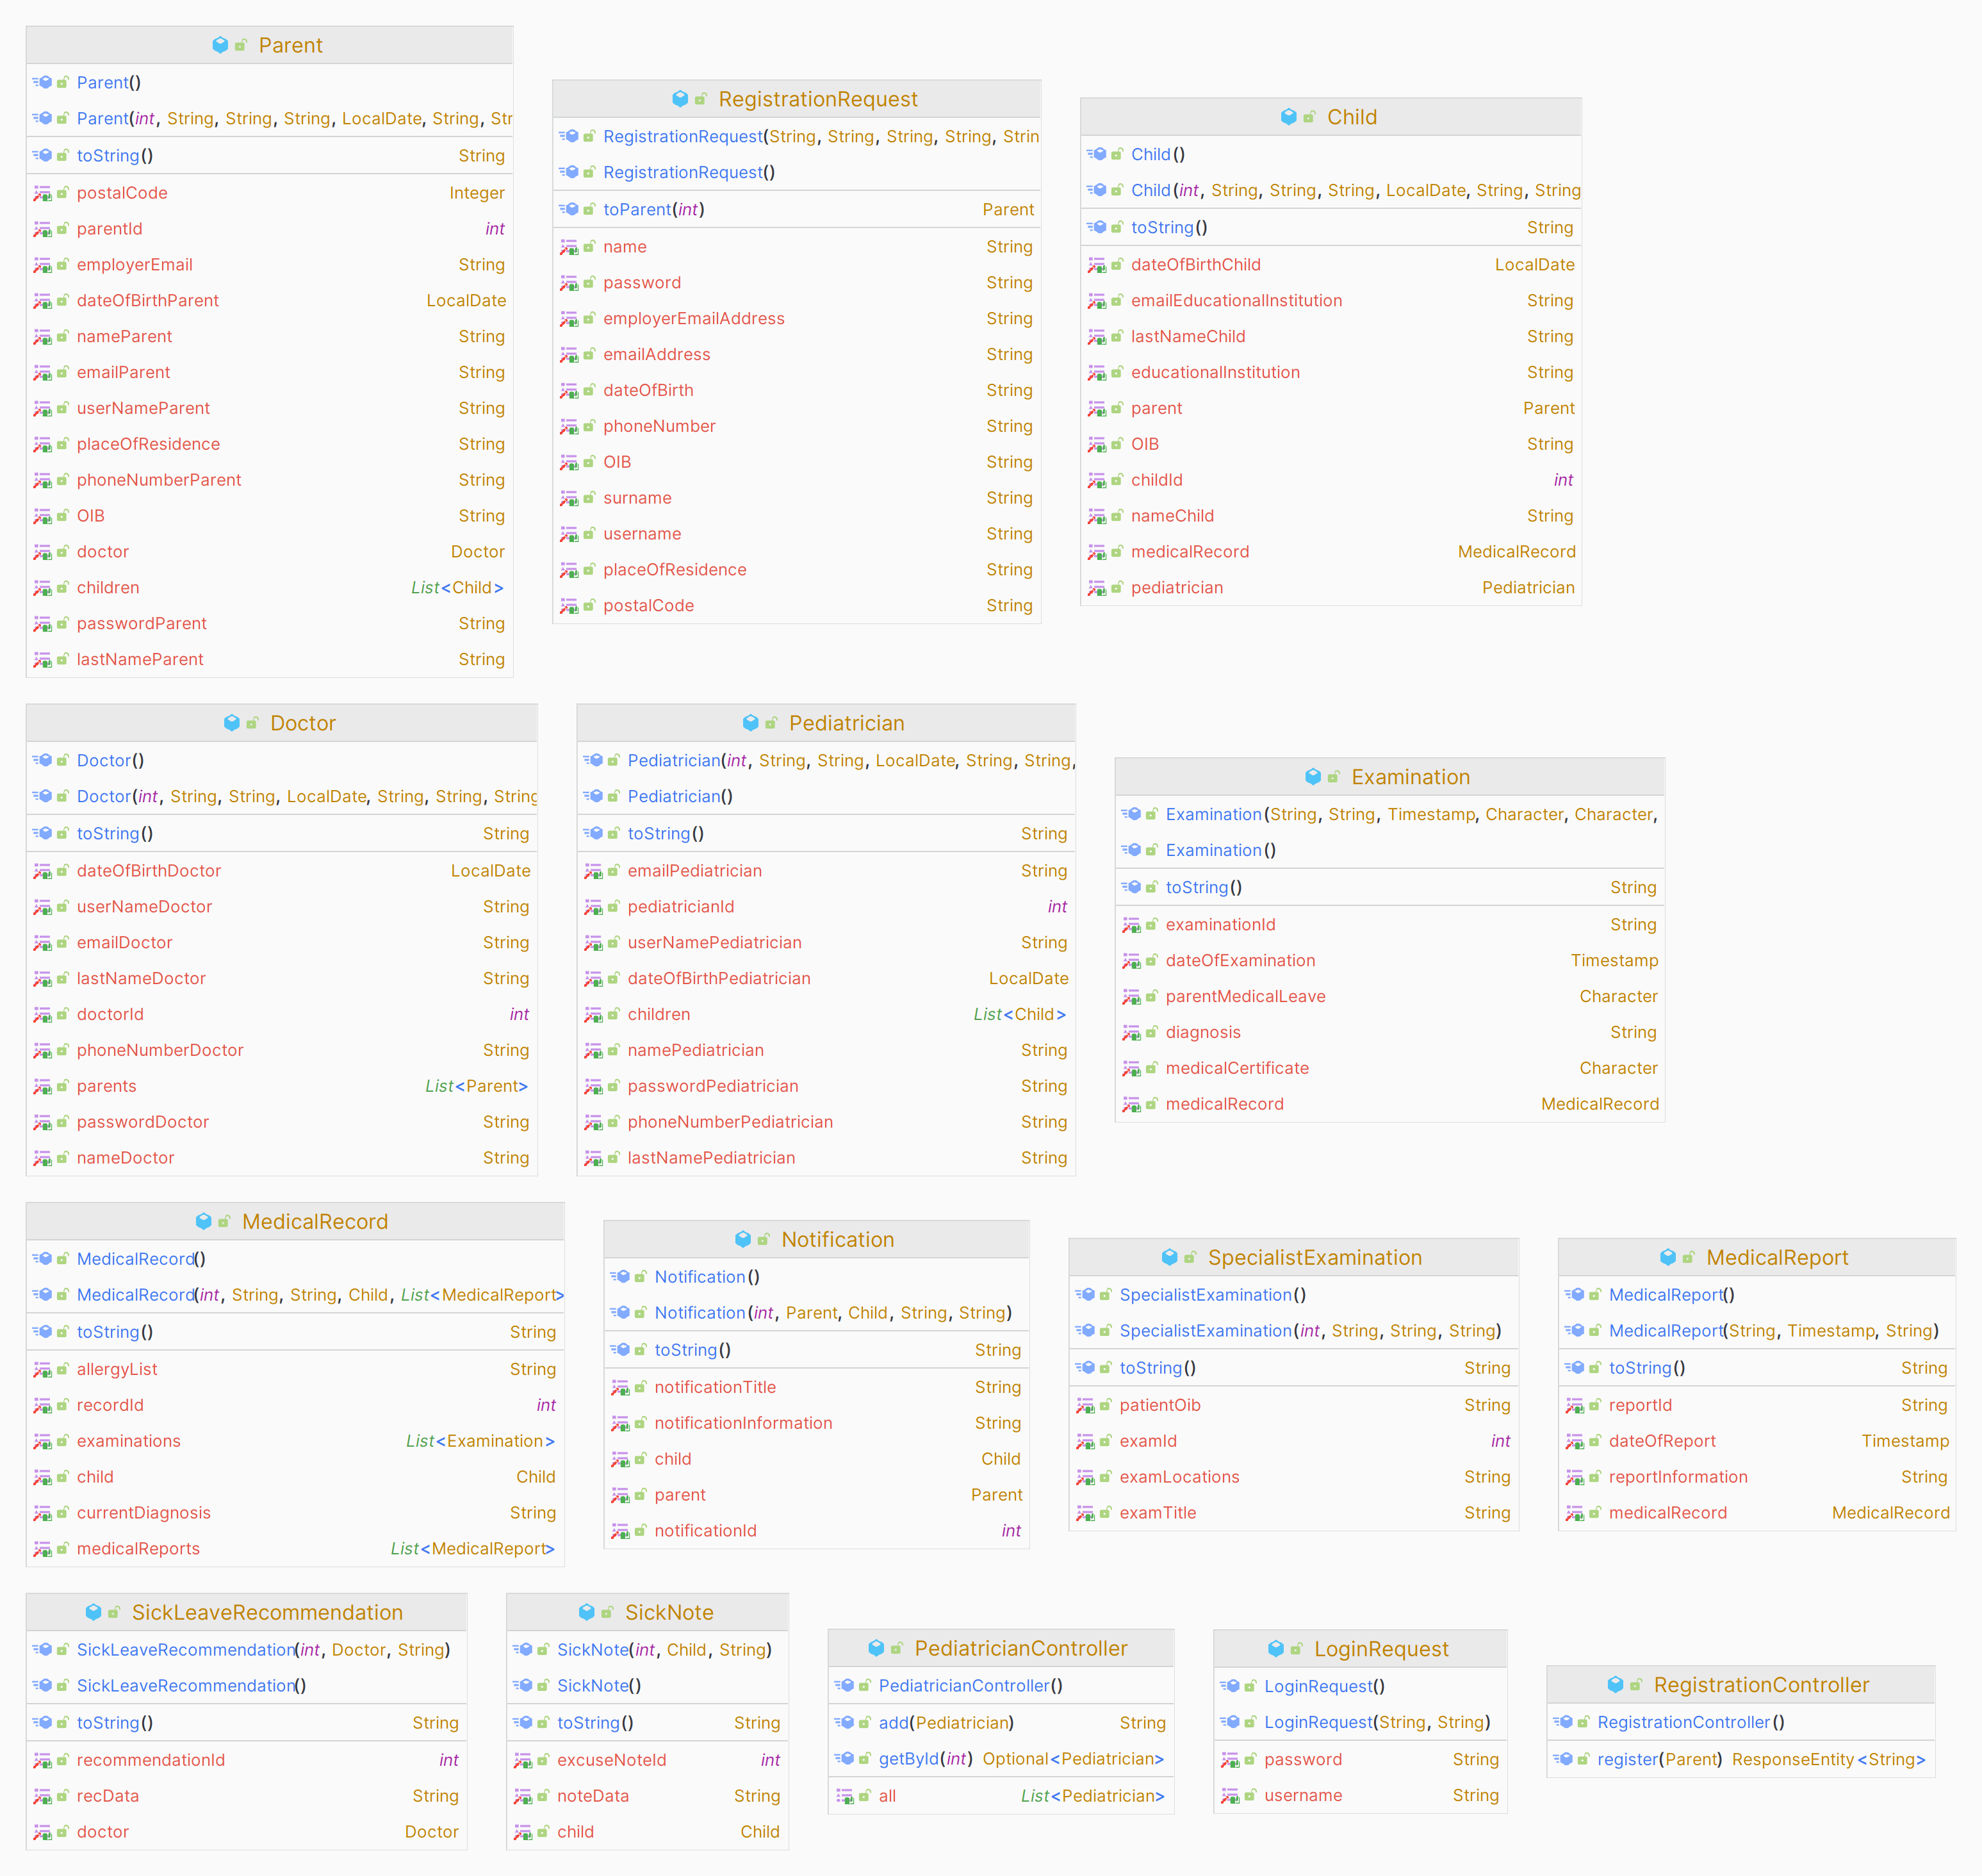
\includegraphics[scale=0.15]{dijagrami/dijraz1.PNG} %veličina slike u odnosu na originalnu datoteku i pozicija slike
				\centering
				\caption{Dijagram razreda 1}
				\label{fig:dijraz1}
			\end{figure}
			\clearpage
			\text Postoje tri razreda koji služe kao kontroleri za manipulaciju objekta i njihovo obrađivanje u bazi podataka za liječnika, pedijatra i roditelja. To su DoctorController, PediatricianController i ParentController. Postoje dva razreda RegistrationController i LoginController koji služe za rukovanje registracijama i prijavama korisnika. Za prijenos podataka između controllera i baze podataka postoje sučelja DoctorService, PediatricianService i ParentService te razredi DoctorServiceImpl, PediatricianServiceImpl i ParentServiceImpl koji implementiraju metode iz tih sučelja i osiguravaju prijenos podataka s bazom podataka preko tri sučelja koji predstavljaju repozitorije: DoctorRepository, PediatricianRepository i ParentRepository.
			%unos slike
			\begin{figure}[H]
				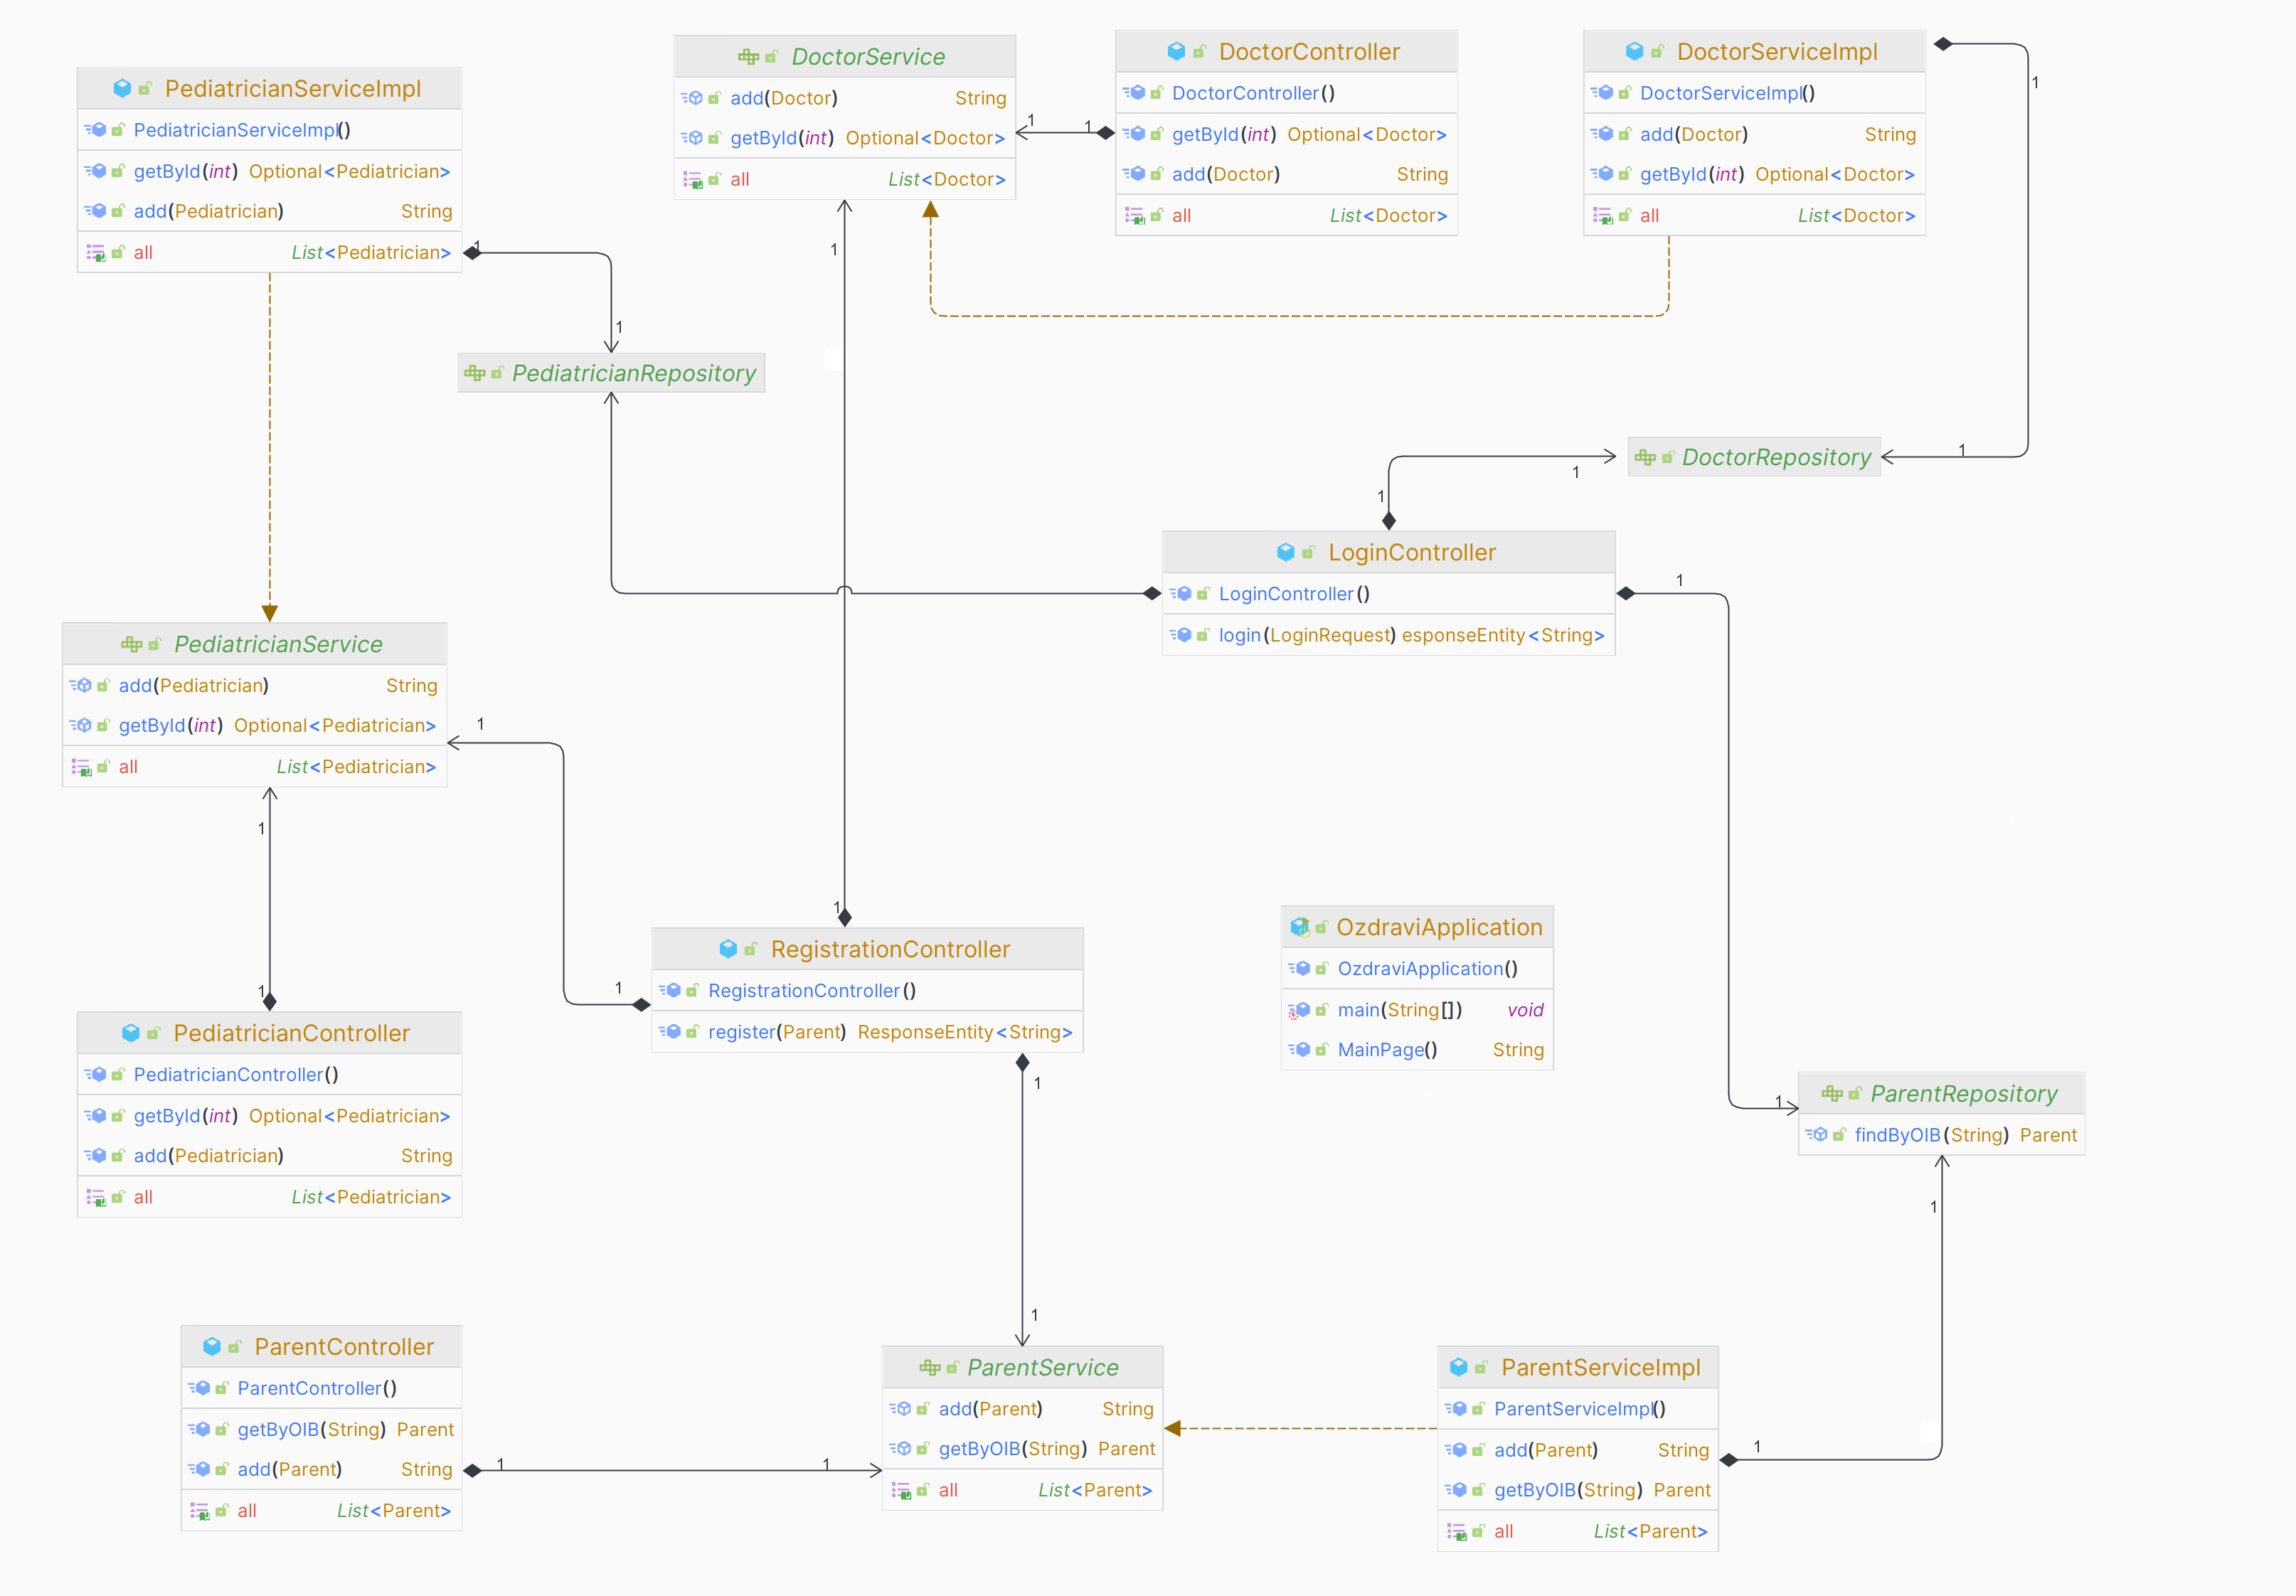
\includegraphics[scale=0.225]{dijagrami/dijraz2.PNG} %veličina slike u odnosu na originalnu datoteku i pozicija slike
				\centering
				\caption{Dijagram razreda 2}
				\label{fig:dijraz2}
			\end{figure} 
			
			%unos slike
			\begin{figure}[H]
				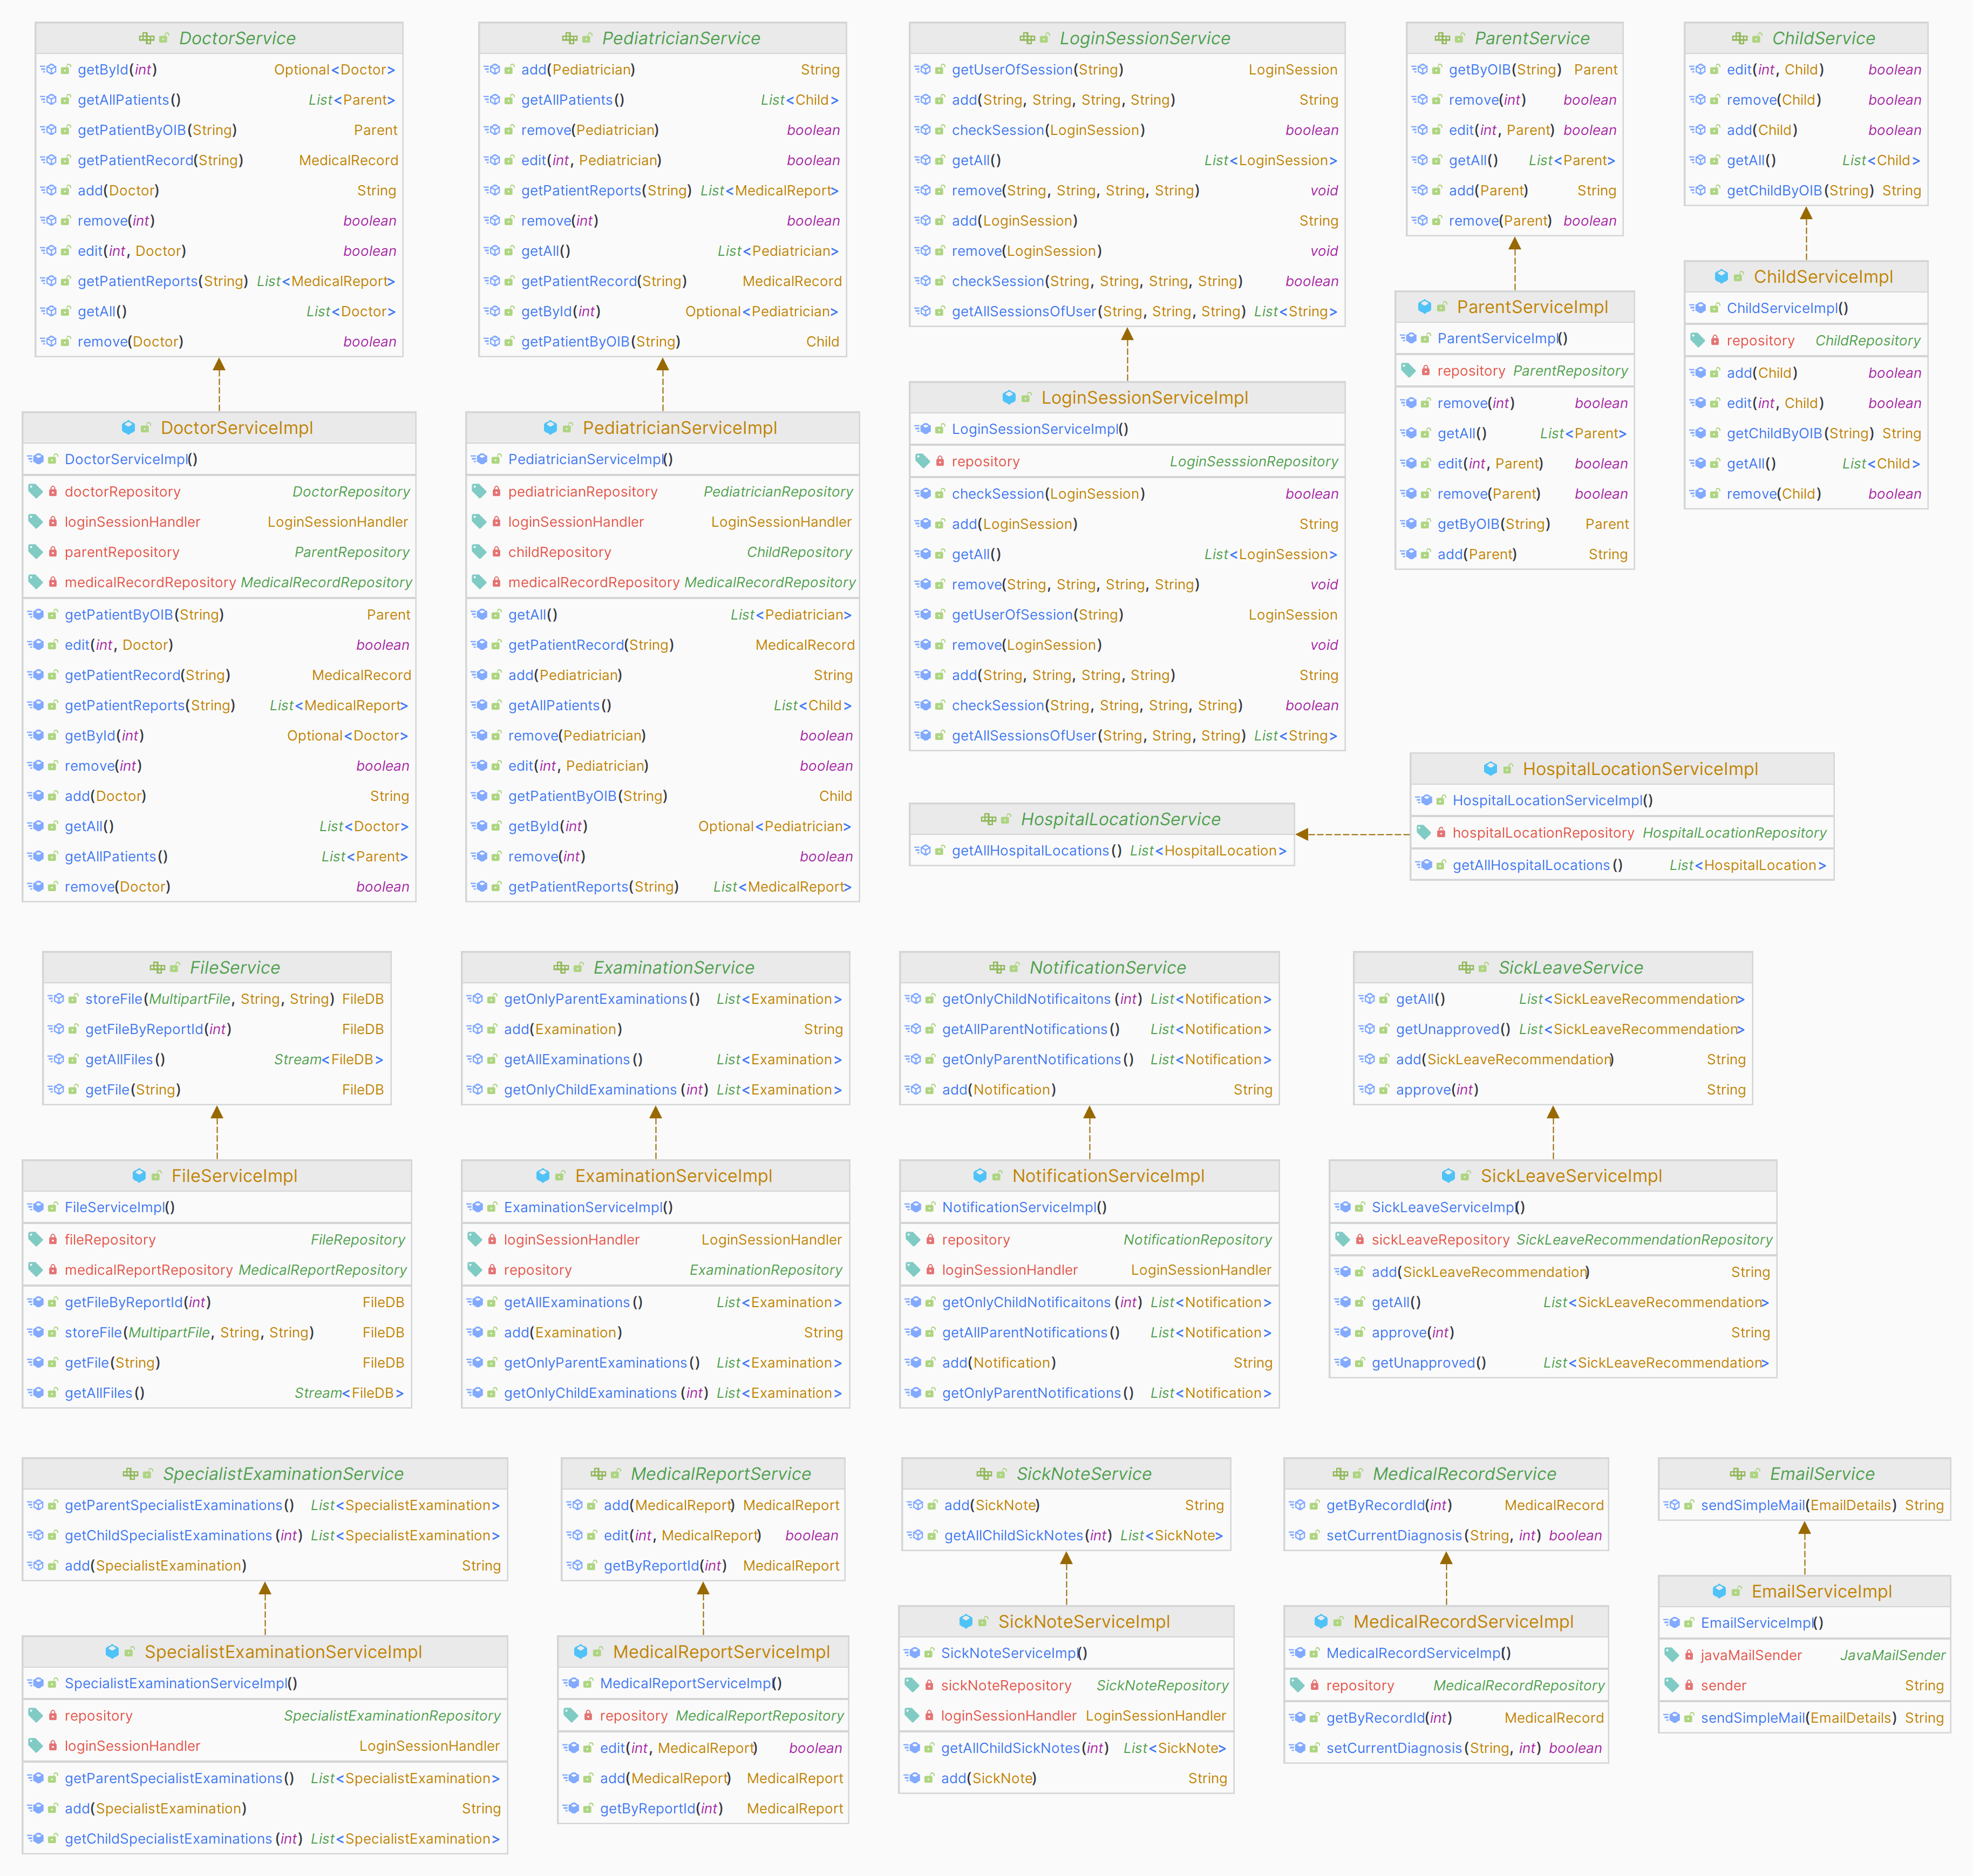
\includegraphics[scale=0.225]{dijagrami/dijraz3.PNG} %veličina slike u odnosu na originalnu datoteku i pozicija slike
				\centering
				\caption{Dijagram razreda 3}
				\label{fig:dijraz3}
			\end{figure}
			
			\textbf{\textit{dio 2. revizije}}\\			
			
			\textit{Prilikom druge predaje projekta dijagram razreda i opisi moraju odgovarati stvarnom stanju implementacije}
			
			
			
			\eject
		
		\section{Dijagram stanja}
			
			
			\textbf{\textit{dio 2. revizije}}\\
			
			\textit{Potrebno je priložiti dijagram stanja i opisati ga. Dovoljan je jedan dijagram stanja koji prikazuje \textbf{značajan dio funkcionalnosti} sustava. Na primjer, stanja korisničkog sučelja i tijek korištenja neke ključne funkcionalnosti jesu značajan dio sustava, a registracija i prijava nisu. }
			
			
			\eject 
		
		\section{Dijagram aktivnosti}
			
			\textbf{\textit{dio 2. revizije}}\\
			
			 \textit{Potrebno je priložiti dijagram aktivnosti s pripadajućim opisom. Dijagram aktivnosti treba prikazivati značajan dio sustava.}
			
			\eject
		\section{Dijagram komponenti}
		
			\textbf{\textit{dio 2. revizije}}\\
		
			 \textit{Potrebno je priložiti dijagram komponenti s pripadajućim opisom. Dijagram komponenti treba prikazivati strukturu cijele aplikacije.}
	\chapter{Implementacija i korisničko sučelje}
		
		
		\section{Korištene tehnologije i alati}
		
			Komunikacija u timu izvedena je putem dva servisa. Korištenjem aplikacije WhatsApp\footnote{https://www.whatsapp.com/}, te na serveru u aplikaciji Discord\footnote{https://discord.com/}. Oboje imaju mogućnosti grupnih poziva, dijeljena ekrana te slanja poruka u grupni \textit{chat}. 
			Za izradu UML dijagrama u dokumentaciji korištena je aplikacija Astah\footnote{https://astah.net/} UML kompanije ChangeVision\footnote{https://www.change-vision.com/}. Za kontrolu verzija izvornog koda korišten je Git\footnote{https://git-scm.com/}, a kao udaljeni repozitorij svog koda i dokumentacije korišten je direktorij na web platformi GitHub\footnote{https://github.com/}.
			Kao razvojno okruženje koristili smo IntelliJ IDEA\footnote{https://www.jetbrains.com/idea/}, integrirano razvojno okruženje (IDE) proizvedeno od strane JetBrains\footnote{https://www.jetbrains.com/}. IntelliJ IDEA koristi se za razvoj aplikacija pisanih u Javi\footnote{https://www.java.com/en/}, Kotlin-u\footnote{https://kotlinlang.org/}, Groovy-u\footnote{https://groovy-lang.org/} i drugim JVM baziranim programskim jezicima.
			Aplikacija je napisana u Java programskom jeziku koristeči alat \textit{Spring Boot}\footnote{https://spring.io/projects/spring-boot/} za razvoj \textit{backenda}, a za razvoj \textit{frontenda} korišten je React\footnote{https://react.dev/}. React je biblioteka programskog jezika JavaScript\footnote{https://www.javascript.com/}, koja se koristi za razvoj programskih sučelja, a stvorio ju je i održava Meta\footnote{https://about.meta.com/}. \textit{Spring Boot} alat je Spring\footnote{https://spring.io/} Framework-a, koji je aplikacijski \textit{framework} za razvoj Java aplikacija, najčešće onih baziranih na rad na web-u.
			Za bazu podataka koristili smo H2\footnote{https://www.h2database.com/html/main.html}, koji je prilagođen radu u Javi i baziran na poslužitelju, za kojeg smo odabrali Render\footnote{https://render.com/}.
			
			\eject 
		
	
		\section{Ispitivanje programskog rješenja}
			
			\textbf{\textit{dio 2. revizije}}\\
			
			 \textit{U ovom poglavlju je potrebno opisati provedbu ispitivanja implementiranih funkcionalnosti na razini komponenti i na razini cijelog sustava s prikazom odabranih ispitnih slučajeva. Studenti trebaju ispitati temeljnu funkcionalnost i rubne uvjete.}
	
			
			\subsection{Ispitivanje komponenti}
			\text Prilikom ispitivanja komponenti izvedeno je 20 testova nad razredima u izvornom kodu. Ovo potpoglavlje biti će ograničeno na svega 6, no ostale je moguće vidjeti na GitHub repozitoriju. Poveznica na isti nalazi se u literaturi. Također, bitno je spomenuti da se sekcija testova naziva \textit{DoctorControllerTest} može gledati kao skupina koja se odnosi i na korisnike tipa Pedijatar i korisnike tipa Liječnik obiteljske medicine, zbog sličnosti izvedbe razreda.
			
			%unos slike
			\begin{figure}[H]
				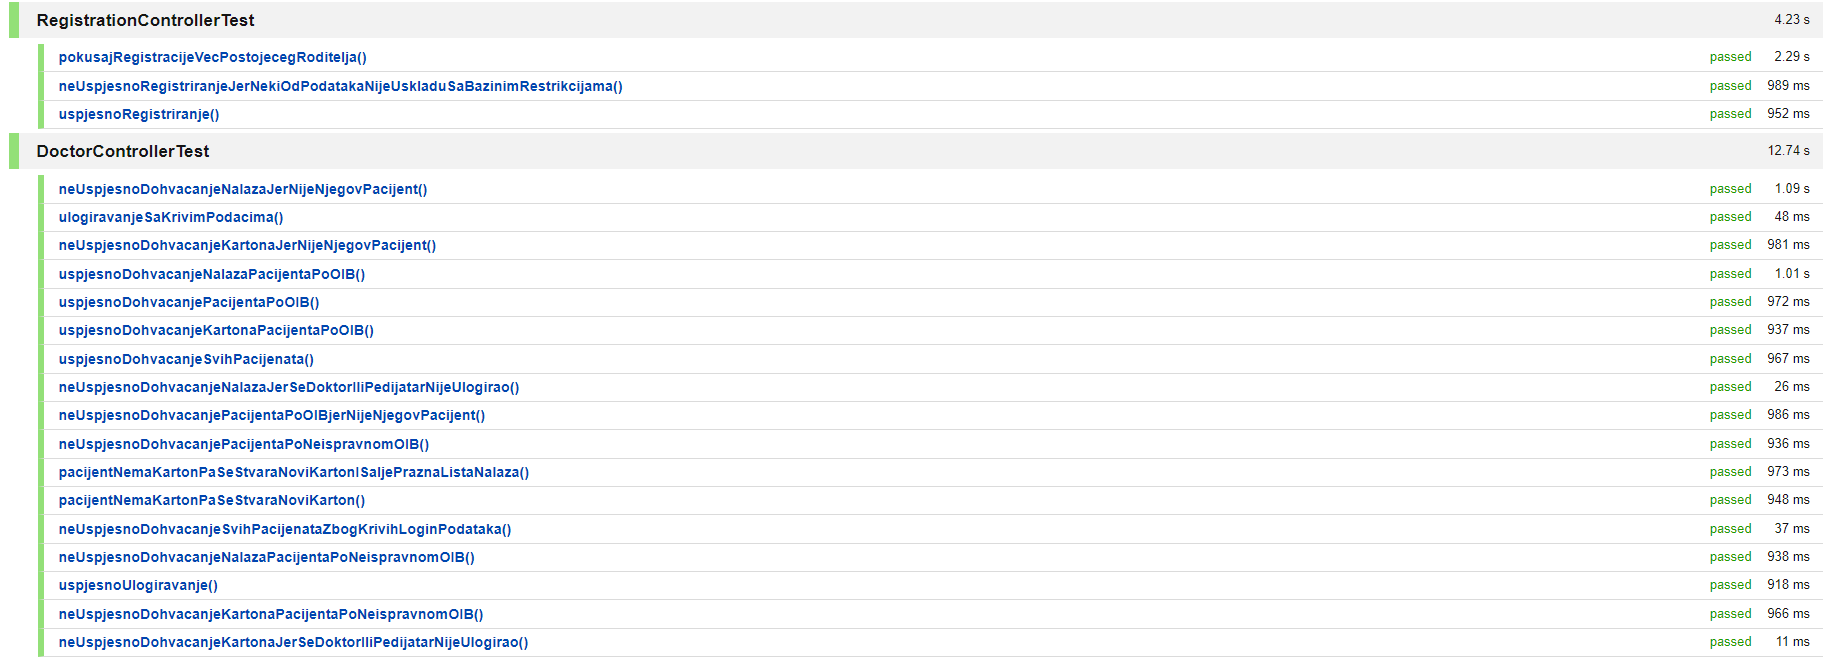
\includegraphics[scale=0.48]{slike/testoviRazreda.PNG} %veličina slike u odnosu na originalnu datoteku i pozicija slike
				\centering
				\caption{Prikaz izvršenih testova}
				\label{fig:slikatestova}
			\end{figure}
			
			\begin{packed_enum}
				
				\item \textbf{Test registracije postojećeg roditelja:}
				\text U navedenom testu šalje se zahtjev za stvaranjem novog entiteta roditelja koji ima već korišteni OIB unutar aplikacije. Očekuje se odgovor tipa "400 Bad Request", kakav odgovor je i dobiven.
				%unos slike
				\begin{figure}[H]
					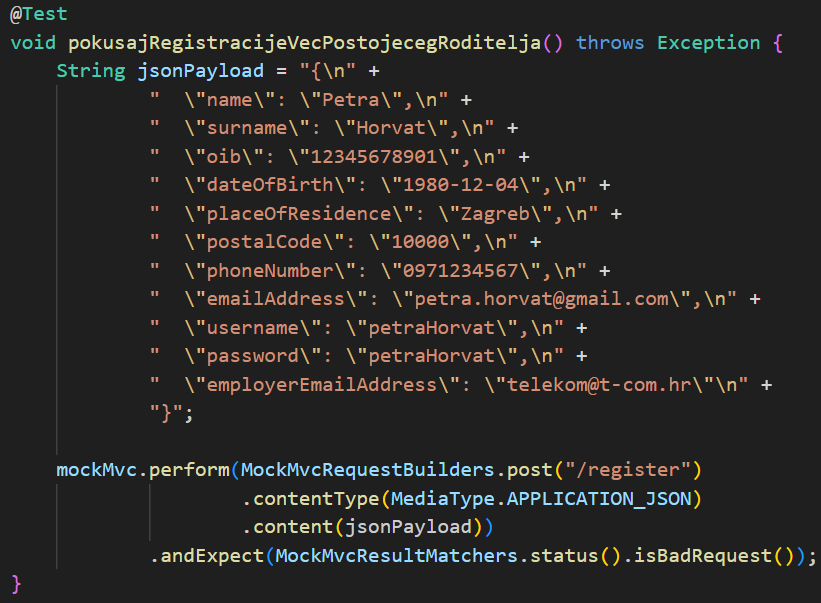
\includegraphics[scale=0.6]{slike/isjecak1.PNG} %veličina slike u odnosu na originalnu datoteku i pozicija slike
					\centering
					\caption{Test registracije postojećeg OIB-a}
					\label{fig:isjecak1}
				\end{figure}
				\item \textbf{Test registracije roditelja:}
				\text U navedenom testu šalje se zahtjev za stvaranjem novog entiteta roditelja, i kojemu su svi podaci ispravni. Očekuje se odgovor tipa "200 OK", kakav je i dobiven.
				%unos slike
				\begin{figure}[H]
					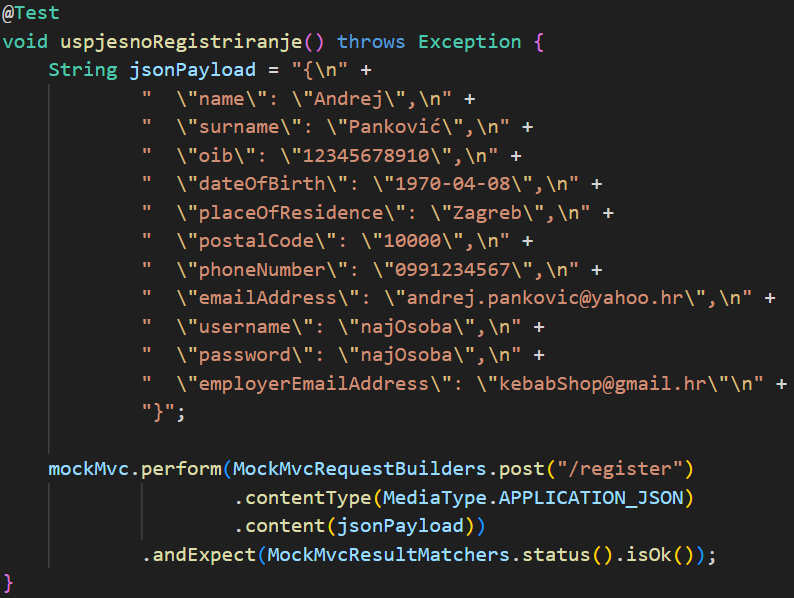
\includegraphics[scale=0.6]{slike/isjecak2.PNG} %veličina slike u odnosu na originalnu datoteku i pozicija slike
					\centering
					\caption{Test registracije roditelja}
					\label{fig:isjecak2}
				\end{figure}
				\item \textbf{Test prijave i dobavljanja svih pacijenata:}
				\text U navedenom testu šalju se ispravni podaci za prijavu, nakon čega se šalje zahtjev za popisom svih pacijenata prijavljenog doktora. Očekuje se odgovor tipa "200 OK", kakav je i dobiven.
				%unos slike
				\begin{figure}[H]
					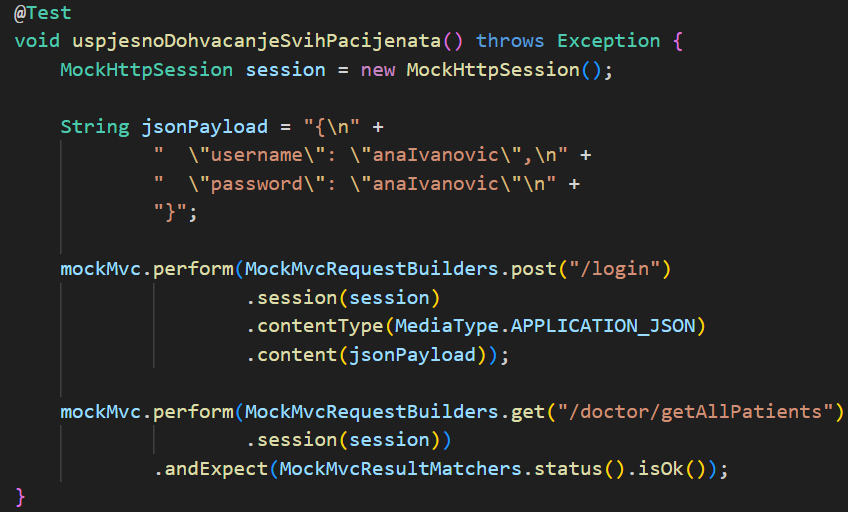
\includegraphics[scale=0.6]{slike/isjecak3.PNG} %veličina slike u odnosu na originalnu datoteku i pozicija slike
					\centering
					\caption{Test dobavljanja pacijenata}
					\label{fig:isjecak3}
				\end{figure}
				\item \textbf{Test dobavljanja kartona:}
				\text U navedenom testu šalju se ispravni podaci za prijavu, nakon čega se šalje zahtjev za kartonom određenog pacijenta. Taj pacijent nema postojeći karton, te je potrebno stvoriti novi. Očekuje se odgovor tipa "200 OK", kakav je i dobiven.
				%unos slike
				\begin{figure}[H]
					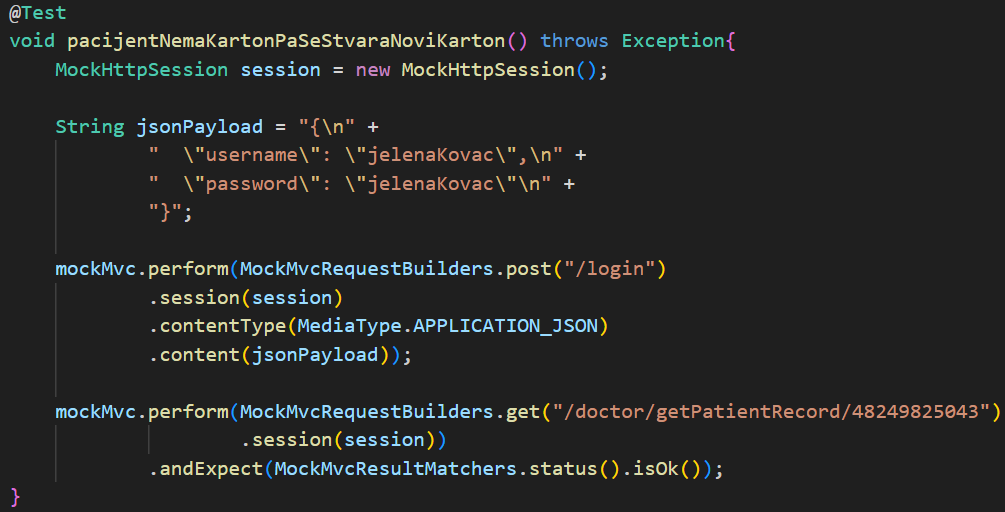
\includegraphics[scale=0.6]{slike/isjecak4.PNG} %veličina slike u odnosu na originalnu datoteku i pozicija slike
					\centering
					\caption{Test dobavljanja kartona}
					\label{fig:isjecak4}
				\end{figure}
				\item \textbf{Test dobavljanja pacijenta po neispravnom OIB-u:}
				\text U navedenom testu šalju se ispravni podaci za prijavu, nakon čega se šalje zahtjev za profilom pacijenta čiji OIB nije unesen u sustav. Očekuje se odgovor tipa "400 Bad Request", kakav je i dobiven.
				%unos slike
				\begin{figure}[H]
					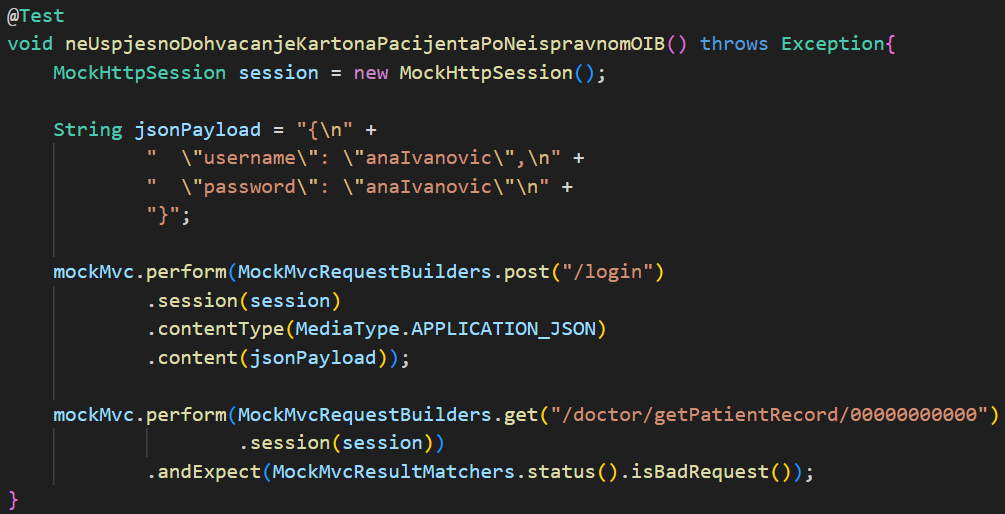
\includegraphics[scale=0.6]{slike/isjecak5.PNG} %veličina slike u odnosu na originalnu datoteku i pozicija slike
					\centering
					\caption{Test dobavljanja pacijenata s neispravnim OIB-om}
					\label{fig:isjecak5}
				\end{figure}
				\item \textbf{Test dobavljanja nalaza pacijenta:}
				\text U navedenom testu šalju se ispravni podaci za prijavu, nakon čega se šalje zahtjev za nalazima pacijenta prijavljenog doktora. Očekuje se odgovor tipa "200 OK", kakav je i dobiven.
				%unos slike
				\begin{figure}[H]
					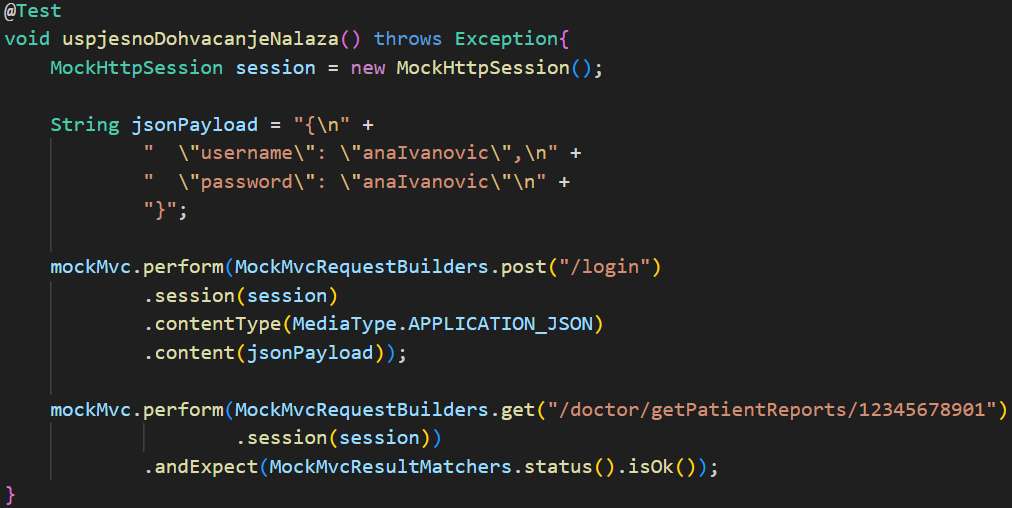
\includegraphics[scale=0.6]{slike/isjecak6.PNG} %veličina slike u odnosu na originalnu datoteku i pozicija slike
					\centering
					\caption{Test dobavljanja nalaza}
					\label{fig:isjecak6}
				\end{figure}
				
			\end{packed_enum}
			\clearpage
			
			
			\subsection{Ispitivanje sustava}
			
			 \textit{Potrebno je provesti i opisati ispitivanje sustava koristeći radni okvir Selenium\footnote{\url{https://www.seleniumhq.org/}}. Razraditi \textbf{minimalno 4 ispitna slučaja} u kojima će se ispitati redovni slučajevi, rubni uvjeti te poziv funkcionalnosti koja nije implementirana/izaziva pogrešku kako bi se vidjelo na koji način sustav reagira kada nešto nije u potpunosti ostvareno. Ispitni slučaj se treba sastojati od ulaza (npr. korisničko ime i lozinka), očekivanog izlaza ili rezultata, koraka ispitivanja i dobivenog izlaza ili rezultata.\\ }
			 
			 \textit{Izradu ispitnih slučajeva pomoću radnog okvira Selenium moguće je provesti pomoću jednog od sljedeća dva alata:}
			 \begin{itemize}
			 	\item \textit{dodatak za preglednik \textbf{Selenium IDE} - snimanje korisnikovih akcija radi automatskog ponavljanja ispita	}
			 	\item \textit{\textbf{Selenium WebDriver} - podrška za pisanje ispita u jezicima Java, C\#, PHP koristeći posebno programsko sučelje.}
			 \end{itemize}
		 	\textit{Detalji o korištenju alata Selenium bit će prikazani na posebnom predavanju tijekom semestra.}
			
			\eject 
		
		
		\section{Dijagram razmještaja}
			
			\text Dijagrami razmještaja spadaju pod strukturne i statičke UML dijagrame koji opisuju topologiju sustava, te su usredotočeni na odnos sklopovskih i programskih dijelova. Na slici 5.X prikazan je dijagram razmještaja naše aplikacije. Na klijentskom se računalu nalazi web preglednik kojim se putem HTTPS veze pristupa aplikaciji. Web aplikacija pokrenuta je unutar web poslužitelja, koji se nalazi na poslužiteljskom računalu. Unutar okoline izvođenja web poslužitelja također se nalazi i baza podataka. Razlog manjku zasebnog poslužitelja za bazu podataka je korištenje baze H2, koja je integrirana u \textit{backend}.
			
			%unos slike
			\begin{figure}[H]
				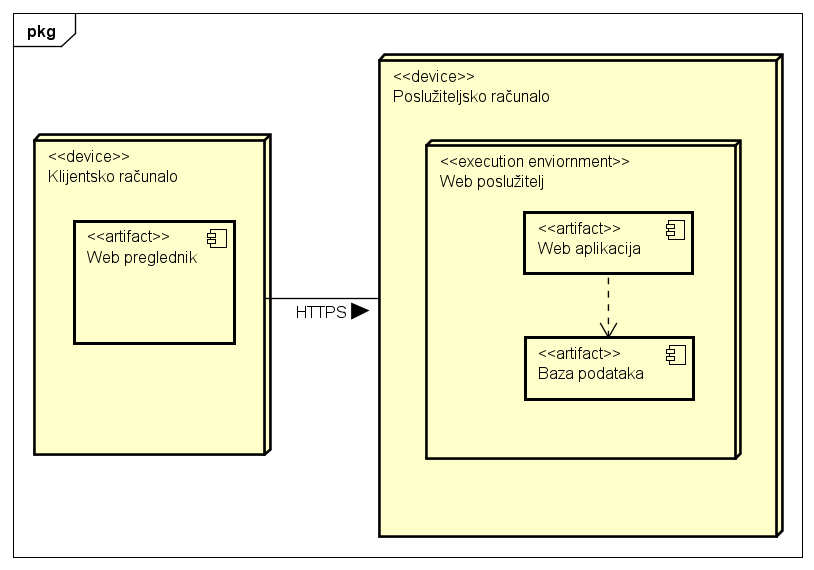
\includegraphics[scale=0.7]{dijagrami/dijrazm1.PNG} %veličina slike u odnosu na originalnu datoteku i pozicija slike
				\centering
				\caption{Dijagram razmještaja}
				\label{fig:dijstanj1}
			\end{figure}
			
			\eject 
		
		\section{Upute za puštanje u pogon}
		
			\subsection{\textit{Deploy} na Render - Backend}
			Potrebno je postaviti izvorni kod aplikacije na vlastiti repozitorij na servisu GitHub. Izvorni kod moguće je preuzeti s GitHub repozitorija projekta, čija se poveznica nalazi u literaturi. Jednom kada je cijeli izvorni kod na repozitoriju, potrebno je otvoriti stranicu servisa Render\footnote{https://dashboard.render.com/}, te se prijaviti ili kreirati račun. Kada je prijava provedena, potrebno je odabrati opciju "New", te odabrati opciju \textit{Web service}.
				%unos slike
			\begin{figure}[H]
				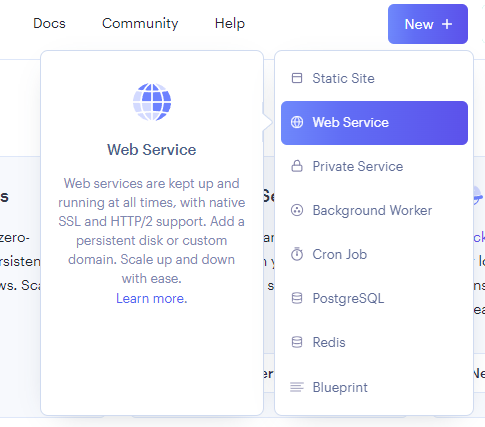
\includegraphics[scale=0.9]{slike/render0.PNG} %veličina slike u odnosu na originalnu datoteku i pozicija slike
				\centering
				\caption{Opcija \textit{Web service}}
				\label{fig:render0}
			\end{figure}
			Nakon toga, potrebno je odabrati prvu opciju na sljedećem izborniku, \textit{Build and deploy from a Git repository}.
			%unos slike
			\begin{figure}[H]
				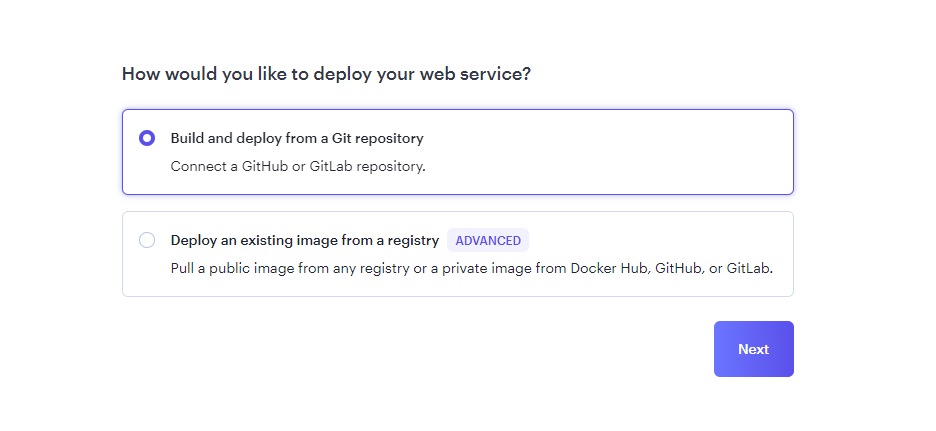
\includegraphics[scale=0.7]{slike/render1.PNG} %veličina slike u odnosu na originalnu datoteku i pozicija slike
				\centering
				\caption{Izbornik za \textit{deploy}}
				\label{fig:render1}
			\end{figure}
			Na idućem ekranu potrebno je prijaviti se pomoću svog GitHub ili GitLab računa. Nakon što se korisnik uspješno prijavi, nudi mu se lista mogućih repozitorija za dodavanje na Render.
			%unos slike
			\begin{figure}[H]
				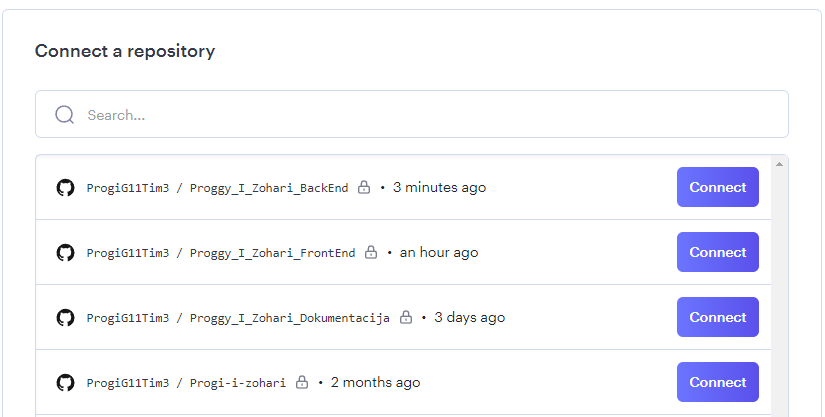
\includegraphics[scale=0.7]{slike/render2.PNG} %veličina slike u odnosu na originalnu datoteku i pozicija slike
				\centering
				\caption{Izbornik repozitorija}
				\label{fig:render2}
			\end{figure}
			Na sljedećem ekranu potrebno je unijeti ime servisa, regiju za korištenje, izvorni/korijenski direktorij te \textit{Runtime} opciju. Pod pretpostavkom da je odabran direktorij za \textit{backend}, unesene opcije trebaju biti sljedeće:
			%unos slike
			\begin{figure}[H]
				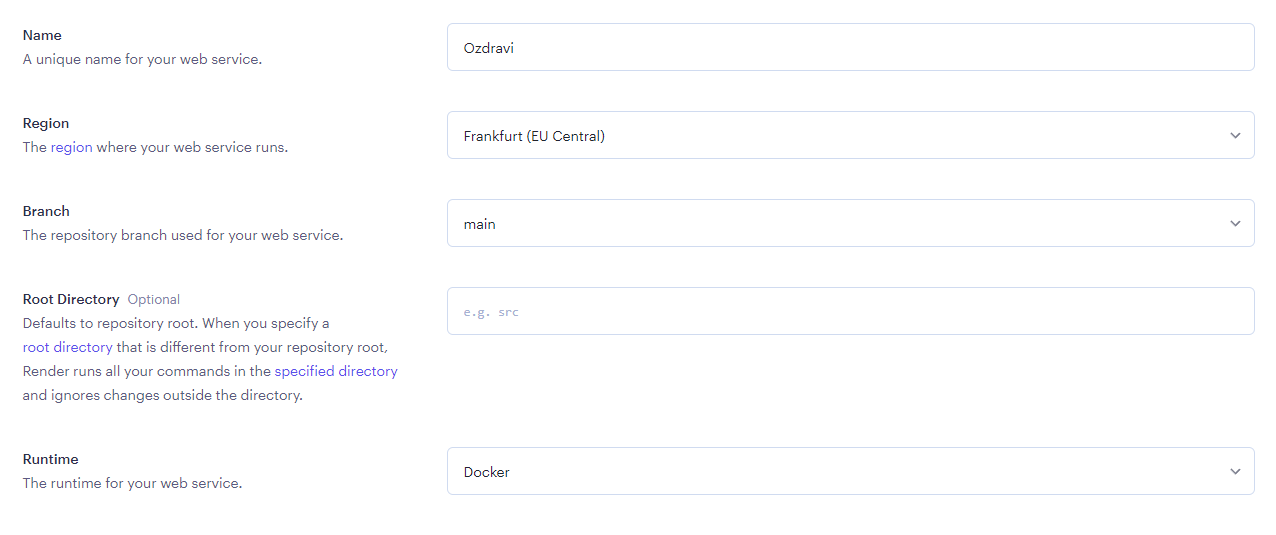
\includegraphics[scale=0.7]{slike/render3.PNG} %veličina slike u odnosu na originalnu datoteku i pozicija slike
				\centering
				\caption{Izbornik opcija za stvaranje \textit{backenda}}
				\label{fig:render3}
			\end{figure}
			Dodatno, potrebno je otvoriti opciju \textit{Advanced} te unijeti putanju do \textit{Dockerfile}, što se u slučaju aplikacije ozdravi nalazi na lokaciji \textbf{./docker/Dockerfile}:
			%unos slike
			\begin{figure}[H]
				
\includegraphics[scale=0.7]{slike/render4.PNG} %veličina slike u odnosu na originalnu datoteku i pozicija slike
				\centering
				\caption{Unos lokacije Dockerfilea}
				\label{fig:render4}
			\end{figure}
			Potrebno je još samo stisnuti gumb \textit{Create Web Service}. \clearpage
			\eject
			
			\subsection{\textit{Deploy} na Render - Frontend}
			Za \textit{deploy} \textit{frontend} dijela aplikacije, potrebno je ponovno odabrati opcije \textbf{New - Web service}. Prilikom unosa opcija, ovaj puta se postupa malo drugačije. Potrebno je unijeti naziv, te dodati \textbf{frontend} kao \textit{root directory}, a zatim odabrati opciju \textit{Node} unutar opcije \textit{Runtime}. Uz to, potrebno je unijeti komandu \textbf{yarn build} unutar opcije \textit{Build Command} i \textbf{yarn start-prod} unutar \textit{Start Command}. 
			%unos slike
			\begin{figure}[H]
				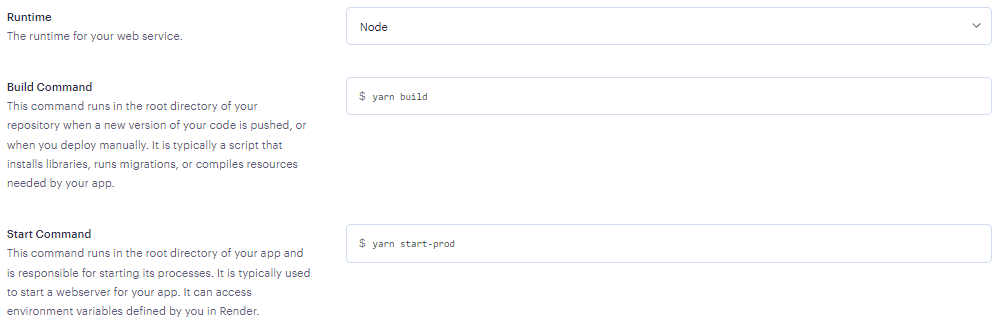
\includegraphics[scale=0.8]{slike/render5.PNG} %veličina slike u odnosu na originalnu datoteku i pozicija slike
				\centering
				\caption{Unos opcija za \textit{frontend}}
				\label{fig:render5}
			\end{figure}
			Potrebno je još samo otvoriti opciju \textit{Advanced}, te u dodatne \textit{environment} varijable dodati varijablu imena\textbf{ API\textunderscore BASE\textunderscore URL}, te postaviti \textit{value} na adresu deployanog backenda aplikacije dostupnu na Render dashboardu.
			%unos slike
			\begin{figure}[H]
				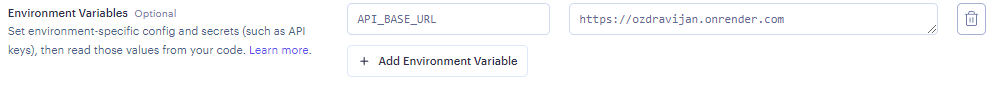
\includegraphics[scale=0.8]{slike/render6.PNG} %veličina slike u odnosu na originalnu datoteku i pozicija slike
				\centering
				\caption{Unos opcije za povezivanje}
				\label{fig:render6}
			\end{figure}
			Ponovno, potrebno je još samo pritisnuti \textit{Create Web Service}.
			
			
			\eject 
	\chapter{Zaključak i budući rad}
		
		\text Zadatak našeg tima na ovome projektu bio je razvoj web aplikacije naziva "Ozdravi". Glavna ideja iza aplikacije jest olakšanje komunikacije između roditelja djece, pedijatara, liječnika obiteljske medicine, škola i poslodavaca. Razvoj aplikacije trajao je 13 tjedana, za vrijeme kojih se dinamika tima i njegova efikasnost drastično mijenjala. Ipak, na kraju je postignut cilj projekta, razvijena je aplikacija. Podijelio bih rad na projektu u tri faze.\\
		Prva faza sastojala se od početne organizacije te nekoliko uzastopnih sastanaka na kojima je razvijana ideja i arhitektura aplikacije, te na kojima su se članovi tima međusobno upoznali. U ovoj fazi izglasan je i voditelj tima, čiju ulogu je preuzeo Jan Komerički. Također, u ovoj fazi su određena 4 pod-tima, svaki sa svojim zadacima. Marko Žaja i Lovro Matić oformili su tim za rad s bazom podataka, koji se u kasnijoj fazi projekta stopio u tim za razvoj \textit{backend} potpore. Taj tim oformili su Dino Dubinović i Luka Bračun. Treći tim sastojao se od Kristine Čavlović i Ante Prolića, koji su odlučili raditi na razvoju potpore za \textit{frontend} dio aplikacije. Zadnji, jednočlani tim sastojao se od Jana Komeričkog, čiji je zadatak postao pisanje kompletne dokumentacije projekta i koordinacija rada ostala tri tima. \\
		Druga faza rada tima bio je razvoj inicijalne verzije aplikacije, a krajnji rok ove faze bio je 17.11.2023. U ovoj fazi su se svi članovi tima upoznali sa tehnologijama koje su bile potrebne za razvoj aplikacije. Fazu je okarakterizirao spor i metodičan rad tima, dijelom zbog još nezrele suradnje među članovima, a dijelom zbog manjka znanja o tehnologijama. Velika većina dokumentacije je također završena u ovoj fazi, te većina UML dijagrama koji su potrebni za prikaz rada aplikacije. Ipak, faza je završila vrlo uspješno, s vrlo pozitivnim povratnim informacijama dionika.\\
		Treća faza rada sastojala se od raspodijele preostalog posla i nastavak rada na razvoju aplikacije. Zadnji tjedan rada bio je pomalo kaotičan zbog ponekad nejasne komunikacije između pod-timova, no projekt i dokumentacija uspješno su završeni.\\
		Ovaj projekt bio je prvi ozbiljni i opsežni projekt razvoja programske potpore za većinu nas. Upoznali smo nove tehnologije, pogotovo \textit{Spring Boot} i \textit{React}, te smo naučili o važnosti dokumentacije. Kvalitetna dokumentacija jedan je od najkorisnijih pomoćnika pri razvoju, jer se po njoj mogu orijentirati svi članovi tima. Sve u svemu, naučili smo kako raditi i komunicirati u timu, te kako se koristiti modernim tehnologijama za programske potpore. Mislim da svi odlazimo od ovog projekta iznimno zadovoljni postignutim, usprkos velikoj količini mogućih unaprijeđenja koja se mogu dodati aplikaciji u budućnosti. ODređeni članovi tima čak su izrazili želju za daljnjim radom unutar ovog tima, ali na nekom vlastitom projektu, tako da je moguće da će \textit{Proggy i Žohari} nastaviti razvijati \textit{software}, bar još neko vrijeme. :)
		
		\eject 
	\chapter*{Popis literature}
		\addcontentsline{toc}{chapter}{Popis literature}
		
		
		\begin{enumerate}
			
			
			\item  Programsko inženjerstvo, FER ZEMRIS, \url{https://www.fer.unizg.hr/predmet/proinz}
			
			\item  I. Sommerville, "Engineering software products : an introduction to modern software engineering", Global ed, Pearson 2021.
			
			\item  A. Jović, M. Horvat, I. Grudenić, "UML-dijagrami: Zbirka primjera i riješenih zadataka", Graphis d.o.o. 2014.
			
			\item  The Unified Modeling Language, \url{https://www.uml-diagrams.org/}
			
			\item  Repozitorij izvornog koda, \url{https://github.com/ProgiG11Tim3/Progi-i-zohari}
			
			\item  W3Schools, \url{https://www.w3schools.com/}
		\end{enumerate}
		
		 
	
	
	\begingroup
	\renewcommand*\listfigurename{Indeks slika i dijagrama}
	%\renewcommand*\listtablename{Indeks tablica}
	%\let\clearpage\relax
	\listoffigures
	%\vspace{10mm}
	%\listoftables
	\endgroup
	\addcontentsline{toc}{chapter}{Indeks slika i dijagrama}


	
	\eject 
		
	\chapter*{Dodatak: Prikaz aktivnosti grupe}
		\addcontentsline{toc}{chapter}{Dodatak: Prikaz aktivnosti grupe}
		
		\section*{Dnevnik sastajanja}
		
		\begin{packed_enum}
			\item  sastanak
			
			\item[] \begin{packed_item}
				\item Datum: 17. listopada 2023.
				\item Prisustvovali: svi članovi tima
				\item Teme sastanka:
				\begin{packed_item}
					\item  prvi sastanak s asistenticom i demonstratorom, te predstavnikom CROZ-a
					\item  kratko predavanje o projektu, generalan plan izvedbe
				\end{packed_item}
			\end{packed_item}
			
			\item  sastanak
			\item[] \begin{packed_item}
				\item Datum: 19. listopada 2023.
				\item Prisustvovali: svi članovi tima
				\item Teme sastanka:
				\begin{packed_item}
					\item  prvi samostalan sastanak
					\item  grupna analiza zadatka, raščišćavanje osnovnih dilema funkcionalnosti
					\item  raspodijela odgovornosti
					\item  odabir alata i tehnologija
				\end{packed_item}
			\end{packed_item}
			
			\item  sastanak
			\item[] \begin{packed_item}
				\item Datum: 24. listopada 2023.
				\item Prisustvovali: svi članovi tima
				\item Teme sastanka:
				\begin{packed_item}
					\item  drugi sastanak s asistenticom i demonstratorom
					\item  prolazak kroz pitanja vezana uz funkcionalnost i izgled aplikacije
					\item  razriješene dileme vezane uz uporabu GitHub-a
				\end{packed_item}
			\end{packed_item}
			\text      \\
			
			\item  sastanak
			\item[] \begin{packed_item}
				\item Datum: 26. listopada 2023.
				\item Prisustvovali: svi članovi tima
				\item Teme sastanka:
				\begin{packed_item}
					\item  drugi samostalni sastanak
					\item  donesene konačne odluke o arhitekturi i izgledu aplikacije
				\end{packed_item}
			\end{packed_item}
			
			\item  sastanak
			\item[] \begin{packed_item}
				\item Datum: 6. studenog 2023.
				\item Prisustvovali: Luka Bračun, Dino Dubinović
				\item Teme sastanka:
				\begin{packed_item}
					\item  sastanak pod-tima za razvoj \textit{backend-a}
					\item  grupno programiranje
				\end{packed_item}
			\end{packed_item}
			
			\item  sastanak
			\item[] \begin{packed_item}
				\item Datum: 7. studenog 2023.
				\item Prisustvovali: Jan Komerički
				\item Teme sastanka:
				\begin{packed_item}
					\item  treći sastanak s asistenticom
					\item  pojašnjen ispravan način pisanja dokumentacije, specifično \textit{use cases}
				\end{packed_item}
			\end{packed_item}
			
			\item  sastanak
			\item[] \begin{packed_item}
				\item Datum: 9. studenog 2023.
				\item Prisustvovali: Luka Bračun, Dino Dubinović, Luka Žaja, Lovro Matić
				\item Teme sastanka:
				\begin{packed_item}
					\item  virtualan sastanak pod-timova za razvoj baze podataka i \textit{backend-a}
					\item  objašnjenje arhitekture baze podataka, te napravljen plan integracije iste s \textit{backend-om}
					\item  vježba korištenja sustava \textit{Postman}
				\end{packed_item}
			\end{packed_item}
			
			\item  sastanak
			\item[] \begin{packed_item}
				\item Datum: 13. studenog 2023.
				\item Prisustvovali: Luka Bračun, Dino Dubinović, Kristina Čavlović, Ante Prolić
				\item Teme sastanka:
				\begin{packed_item}
					\item  virtualan sastanak pod-timova za razvoj \textit{frontend-a} i \textit{backend-a}
					\item  rad s login i registracija funkcionalnostima
				\end{packed_item}
			\end{packed_item}
			
			\item  sastanak
			\item[] \begin{packed_item}
				\item Datum: 15. studenog 2023.
				\item Prisustvovali: Dino Dubinović, Kristina Čavlović, Ante Prolić, Jan Komerički
				\item Teme sastanka:
				\begin{packed_item}
					\item  virtualan sastanak pod-timova za razvoj \textit{frontend-a} i \textit{backend-a}, te voditelja tima
					\item  rad s login i registracija funkcionalnostima
				\end{packed_item}
			\end{packed_item}
			
			\item  sastanak
			\item[] \begin{packed_item}
				\item Datum: 16. studenog 2023.
				\item Prisustvovali: svi članovi tima
				\item Teme sastanka:
				\begin{packed_item}
					\item  virtualan sastanak cijelog tima
					\item  prikaz rada aplikacije, \textit{deployment}
				\end{packed_item}
			\end{packed_item}
			%
			
		\end{packed_enum}
		
		\eject
		\section*{Tablica aktivnosti}
		

			\begin{longtblr}[
					label=none,
				]{
					vlines,hlines,
					width = \textwidth,
					colspec={X[7, l]X[1, c]X[1, c]X[1, c]X[1, c]X[1, c]X[1, c]X[1, c]}, 
					vline{1} = {1}{text=\clap{}},
					hline{1} = {1}{text=\clap{}},
					rowhead = 1,
				} 
			
				\SetCell[c=1]{c}{} & \SetCell[c=1]{c}{\rotatebox{90}{\textbf{Jan Komerički}}} & \SetCell[c=1]{c}{\rotatebox{90}{\textbf{Luka Bračun }}} &	\SetCell[c=1]{c}{\rotatebox{90}{\textbf{Kristina Čavlović }}} & \SetCell[c=1]{c}{\rotatebox{90}{\textbf{Dino Dublinović }}} &	\SetCell[c=1]{c}{\rotatebox{90}{\textbf{Lovro Matić }}} & \SetCell[c=1]{c}{\rotatebox{90}{\textbf{Ante Prolić }}} &	\SetCell[c=1]{c}{\rotatebox{90}{\textbf{Luka Žaja }}} \\  
				Upravljanje projektom 		& 8 &  &  &  &  &  & \\ 
				Opis projektnog zadatka 	& 4 &  &  &  &  &  & \\ 
				
				Funkcionalni zahtjevi       & 3 &  &  &  &  &  &  \\ 
				Opis pojedinih obrazaca 	& 14 &  &  &  &  &  &  \\ 
				Dijagram obrazaca 			& 3 &  &  &  &  &  &  \\ 
				Sekvencijski dijagrami 		& 8 &  &  &  &  &  &  \\ 
				Opis ostalih zahtjeva 		& 0.5 &  &  &  &  &  &  \\ 

				Arhitektura i dizajn sustava	 & 5 & 5 & 5 & 5 & 5 & 5 & 5 \\ \hline
				Opis baza podataka 	& 7.5 &  &  &  &  &  &   \\ 
				Dijagrami baza podataka				&  &  &  &  & 3 &  & 3  \\ 
				Dijagram razreda 			&  & 4 &  &  &  &  &   \\ 
				Dijagram stanja				&  &  &  &  &  &  &  \\ 
				Dijagram aktivnosti 		&  &  &  &  &  &  &  \\ 
				Dijagram komponenti			&  &  &  &  &  &  &  \\ 
				Korištene tehnologije i alati 		&  &  &  &  &  &  &  \\ 
				Ispitivanje programskog rješenja 	&  &  &  &  &  &  &  \\ 
				Dijagram razmještaja			&  &  &  &  &  &  &  \\ 
				Upute za puštanje u pogon 		&  &  &  &  &  &  &  \\  
				Dnevnik sastajanja 			&  &  &  &  &  &  &  \\ 
				Zaključak i budući rad 		&  &  &  &  &  &  &  \\  
				Popis literature 			&  &  &  &  &  &  &  \\  
				\textit{vizualni dizajn aplikacije} 				&  &  & 9 &  &  &  &  \\  
				\textit{projektiranje baze podataka} 				&  &  &   &  &  &  & 4 \\ 
				\textit{izrada baze podataka} 		 			&  &  &  &  & 15 &  & \\  
				\textit{spajanje s bazom podataka} 							&  &  &  &  &  &  &  \\ 
				\textit{back end} 							&  & 15 &  & 20 &  &  & 15 \\  
				\textit{front end}				&  &  & 9 &  &  & 22 & \\ 
				\textit{puštanje u pogon}    &  &  &  &  &  &  &  \\
			\end{longtblr}
					
					
		\eject
		\section*{Dijagrami pregleda promjena}
		
		\textbf{\textit{dio 2. revizije}}\\
		
		\textit{Prenijeti dijagram pregleda promjena nad datotekama projekta. Potrebno je na kraju projekta generirane grafove s gitlaba prenijeti u ovo poglavlje dokumentacije. Dijagrami za vlastiti projekt se mogu preuzeti s gitlab.com stranice, u izborniku Repository, pritiskom na stavku Contributors.}
		
	


\end{document} %naredbe i tekst nakon ove naredbe ne ulaze u izgrađen dokument 


